%%%%%%%%%%%%%%%%%%%%%%%%%%%%%%%%%%%%%%%%%%%%%%%%%%%%%%%%%%%%%%%%%%%
%                                                                 %
%   ZEBRA - Reference Manual -- LaTeX Source                      %
%                                                                 %
%   Main driver file. Includes other files of manual,             %
%   generates table of contents and includes index file.          %
%                                                                 %
%   Contains an description of the ZEBRA system                   %
%                                                                 %
%   Files referenced: zebfront.tex    front material              %
%                     zebintr.tex     introduction to zebra       %
%                     zebmz1 to 5.tex MZ reference section        %
%                     zebfz1 to 5.tex FZ reference section        %
%                     zebrz1 to 2.tex RZ reference section        %
%                     zebdz1 to 2.tex DZ reference section        %
%                     zebdzd1.tex     DZDOC reference section     %
%                     zebdia.tex      MZ and FZ diagnostics       %
%                     zebmza.tex      MZ appendix                 %
%                     zebrza.tex      RZ appendix                 %
%                     zebramain.bbl   bibliography information    %
%                                     uses cnasbibl.bib and       %
%                                          textproc.bib           %
%                                                                 %
%   To run, you need the CERN styles cernman.sty and cernman.sty  %
%                                                                 %
%   Editor: Michel Goossens / CN-AS                               %
%   Last Mod.:  6 August 1993 12:00 mg                            %
%                                                                 %
%%%%%%%%%%%%%%%%%%%%%%%%%%%%%%%%%%%%%%%%%%%%%%%%%%%%%%%%%%%%%%%%%%%

\documentstyle[11pt,epsfig,longtable,changebar,portlandps,cerndoc]{cernman}
\newcommand{\FZfile}{FZ~file\index{FZ!Sequential input/output}\index{input/output!FZ}}
\newcommand{\RZfile}{RZ~file\index{RZ!Random input/output}\index{input/output!RZ}}
\newcommand{\IQUEST}{\Lit{IQUEST}%
  \index{IQUEST@{\tt IQUEST}!user communication vector in common {\tt QUEST}}%
  \index{IQUEST@{\tt IQUEST}!error reporting}\index{error reporting!{\tt IQUEST}}%
  \index{QUEST@{\tt QUEST}!user communication common}}
\newcommand{\QUEST}{\Lit{QUEST}%
  \index{IQUEST@{\tt IQUEST}!user communication vector in common {\tt QUEST}}%
  \index{IQUEST@{\tt IQUEST}!error reporting}\index{error reporting!{\tt IQUEST}}%
  \index{QUEST@{\tt QUEST}!user communication common}}
\driver{DVIPS}
\setlongtables
\makeindex
\def\landscape{}
\def\portrait{}
\renewenvironment{landscapebody}{}{}
\psdraft
\PScommands% Initialize PS boxes
\setcounter{secnumdepth}{3}
\setcounter{tocdepth}{2}
\begin{document}
%  ==================== Front material ============================
%%%%%%%%%%%%%%%%%%%%%%%%%%%%%%%%%%%%%%%%%%%%%%%%%%%%%%%%%%%%%%%%%%%
%                                                                 %
%   ZEBRA DZ - Reference Manual -- LaTeX Source                   %
%                                                                 %
%   Front Material: Title page,                                   %
%                   Copyright Notice                              %
%                   Preliminary Remarks                           %
%                   Table of Contents                             %
%   EPS files     : cernlogo.eps, cnastit.eps                     %
%                                                                 %
%   Editor: Michel Goossens / CN-AS                               %
%   Last Mod.: 27 Jan 1995  9:00 mg                               %
%                                                                 %
%%%%%%%%%%%%%%%%%%%%%%%%%%%%%%%%%%%%%%%%%%%%%%%%%%%%%%%%%%%%%%%%%%%

%%%%%%%%%%%%%%%%%%%%%%%%%%%%%%%%%%%%%%%%%%%%%%%%%%%%%%%%%%%%%%%%%%%%
%    Tile page                                                     %
%%%%%%%%%%%%%%%%%%%%%%%%%%%%%%%%%%%%%%%%%%%%%%%%%%%%%%%%%%%%%%%%%%%%
\def\Ptitle#1{\special{ps: /Printstring (#1) def}
                       \epsfbox{cnastit.eps}}
\begin{titlepage}
\vspace*{-23mm}

\includegraphics[height=30mm]{cern15.eps}%
\hfill
\raisebox{8mm}{\Large\bf CERN Program Library Long Writeups Q100/Q101}
\hfill\mbox{}
\begin{center}
\mbox{}\\[6mm]
\mbox{\Ptitle{ZEBRA}}\\[2cm]
{\LARGE Overview of the ZEBRA System}\\[4mm]
{\LARGE MZ -- Memory Management}\\[4mm]
{\LARGE FZ -- Sequential Input/Output}\\[4mm]
{\LARGE RZ -- Random-access Input/Output}\\[4mm]
{\LARGE DZ -- Debugging Tools}\\[4mm]
{\LARGE DZDOC -- Bank documentation tools}\\[4mm]
{\LARGE TZ -- Title Handling}\\[4mm]
{\LARGE JZ91 -- Processor Support}\\[4mm]
{\LARGE Error Diagnostics}\\[25mm]
\end{center}
\vfill
\begin{center}\Large CERN Geneva, Switzerland\end{center}
\end{titlepage}

%%%%%%%%%%%%%%%%%%%%%%%%%%%%%%%%%%%%%%%%%%%%%%%%%%%%%%%%%%%%%%%%%%%%
%    Copyright  page                                               %
%%%%%%%%%%%%%%%%%%%%%%%%%%%%%%%%%%%%%%%%%%%%%%%%%%%%%%%%%%%%%%%%%%%%
\thispagestyle{empty}
\framebox[\textwidth][t]{\hfill\begin{minipage}{0.96\textwidth}%
\vspace*{3mm}
\begin{center}Copyright Notice\end{center}
\setlength{\parskip}{.6\baselineskip}

CERN Program Library entries \textbf{Q100} and \textbf{Q101}
 
\textbf{The ZEBRA system}

\copyright{} Copyright CERN, Geneva 1995
 
Copyright and any other appropriate legal protection of these
computer programs and associated documentation reserved in all
countries of the world.
 
These programs or documentation may not be reproduced by any
method without prior written consent of the Director-General
of CERN or his delegate.
 
Permission for the usage of any programs described herein is
granted apriori to those scientific institutes associated with
the CERN experimental program or with whom CERN has concluded
a scientific collaboration agreement.
 
Requests for information should be addressed to:
\vspace*{-.5\baselineskip}
\begin{center}\ttfamily
\begin{tabular}{l}
CERN Program Library Office              \\
CERN-CN Division                         \\
CH-1211 Geneva 23                        \\
Switzerland                              \\
Tel.      +41 22 767 4951                \\
Fax.      +41 22 767 8630                \\
Internet: cernlib@cern.ch
\end{tabular}
\end{center}
\vspace*{2mm}
\end{minipage}\hfill}%end of minipage in framebox
\vspace{6mm}
 
{\bf Trademark notice: All trademarks appearing in this guide are acknowledged as such.}
\vfill

\begin{tabular}{l@{\quad}l@{\quad}>{\small\tt}l}
{\em Contact Persons\/}: general        & Jamie Shiers /CN      & (shiers\atsign cern.ch)  \\
\phantom{\em Contact Persons\/}: FZ, MZ, TZ, JZ91 & Julius Zoll /ECP & (zoll\atsign cern.ch)  \\
\phantom{\em Contact Persons\/}: DZDOC  & Otto Schaile/PPE-Opal & (o.schaile\atsign cern.ch)\\[1mm]
\textem{Technical Realization\/}:       & Michel Goossens /CN   & (goossens\atsign cern.ch)\\[1cm]
\textem{Edition -- February 1995}
\end{tabular}
\newpage

%%%%%%%%%%%%%%%%%%%%%%%%%%%%%%%%%%%%%%%%%%%%%%%%%%%%%%%%%%%%%%%%%%%%
%    Introductory material                                         %
%%%%%%%%%%%%%%%%%%%%%%%%%%%%%%%%%%%%%%%%%%%%%%%%%%%%%%%%%%%%%%%%%%%%

\pagenumbering{roman}
\setcounter{page}{1}

\section*{Preliminary remarks}

This manual consists of several parts:

\begin{Itemize}
\item An overview of the ZEBRA system.
\item A reference section with a description of the DZ, MZ, FZ, 
      JZ91, RZ and TZ packages.
\item An example program showing how to use the MZ and DZ routines of ZEBRA.
\item A description of the DZDOC documentation system.
\item A list of the diagnostics messages generated by the FZ and MZ
      parts of the ZEBRA system.
\end{Itemize}

\subsection*{Conventions}

In this manual
examples are in \texttt{monotype face} and strings to be input by the user 
are {\Ucom{underlined}}.
In the index the page where a routine is defined is in {\bf bold},
page numbers where a routine is referenced are in normal type.

This manual flags output parameters in subroutine calls,
i.e. parameters which return values to the caller,
by an asterisk \Lit{"*"} following the argument's name.
If the input value of such a parameter is also significant
this is marked by prefixing a second asterisk.
A parameter which is a link is marked by an exclamation mark \Lit{"!"}.

The types of variables follow from the Fortran default typing
convention, except that variables beginning with the letters
"{\tt ch}" are of type {\tt CHARACTER}. 

The Fortran labelled \Lit{COMMON /\QUEST/IQUEST(100)} serves
for communication between the Zebra system and the user,
and also as scratch area in Zebra.

This document has been produced using \LaTeX~\cite{bib-LATEX}
with the \Lit{cernman} style option, developed at CERN. 
A gzipped compressed PostScript file \Lit{zebra.ps.gz}, 
containing a complete printable version
of this manual, can be obtained by anonymous ftp as follows
(commands to be typed by the user are underlined)%
\footnote{If you do not have the gnu {\tt gunzip} utility on your system
          you can get the uncompressed PostScript version by typing the
          command \Ucom{get zebra.ps}, without the {\tt gz} suffix. 
          In order to save Internet bandwidth, you are, however, strongly 
          urged to try and install the {\tt gunzip} utility since gzipped files 
          are about three times smaller than their unzipped equivalents.}:

\vspace*{3mm} 
\begin{XMP}
    \Ucom{ftp asisftp.cern.ch}
    Trying 128.141.201.136...
    Connected to asis01.cern.ch.
    220 asis01 FTP server (Version 6.10 ...) ready.
    Name (asis01:username): \Ucom{anonymous}
    Password: \Ucom{your\_{}mailaddress}
    230 Guest login ok, access restrictions apply.
    ftp> \Ucom{cd cernlib/doc/ps.dir}
    ftp> \Ucom{binary}
    ftp> \Ucom{get zebra.ps.gz}
    ftp> \Ucom{quit}
\end{XMP}
\vspace*{3mm} 

\newpage

%%%%%%%%%%%%%%%%%%%%%%%%%%%%%%%%%%%%%%%%%%%%%%%%%%%%%%%%%%%%%%%%%%%%
%    Tables of contents ...                                        %
%%%%%%%%%%%%%%%%%%%%%%%%%%%%%%%%%%%%%%%%%%%%%%%%%%%%%%%%%%%%%%%%%%%%
\tableofcontents
\listoffigures
\cleardoublepage
%\listoftables

% Local Variables: 
% mode: latex
% TeX-master: "zebramain"
% End: 

%  ==================== Body of text ==============================
\pagenumbering{arabic}
\setcounter{page}{1}
\part{An Introduction to the ZEBRA system}
%%%%%%%%%%%%%%%%%%%%%%%%%%%%%%%%%%%%%%%%%%%%%%%%%%%%%%%%%%%%%%%%%%%
%                                                                 %
%   ZEBRA User Guide -- LaTeX Source                              %
%                                                                 %
%   Chapter Introduction                                          %
%                                                                 %
%   The following external EPS files are referenced:              %
%   linstru , genstru , zeblink , bnkform , relocat               %
%                                                                 %
%   Editor: Michel Goossens / CN-AS                               %
%   Last Mod.: 29 Sep. 1993 20:30  mg                             %
%                                                                 %
%%%%%%%%%%%%%%%%%%%%%%%%%%%%%%%%%%%%%%%%%%%%%%%%%%%%%%%%%%%%%%%%%%%

\Filename{H1ZEBRA-An-overview}

\chapter{ZEBRA - An overview}

\Filename{H2Intro-Why-ZEBRA}
\section{Why ZEBRA?}

All off-line programming in high-energy physics is carried out, for
various reasons, in the Fortran~77 programming language. While this
language offers certain advantages over its competitors, it does suffer
from one serious defect, namely its lack of dynamic data structuring
facilities. The only data structures it contains at all are the array of
homogeneous elements and the common block for shared data. Neither of
these structures can be manipulated as an entity, and neither of them
can be defined dynamically at execution-time. No pointers are available
to link these structures together at a higher level.
If we were to attempt to
define structures using standard Fortran they would thus, at best, be in
the following style:

\begin{XMPt}{Example of defining data structure with Fortran}
      PARAMETER (NTRACKS = 100 , NPTS = 20)
      COMMON/POINTS/PTRACK(3,NTRACK),XYZ(NPTS,NTRACK),...
\end{XMPt}

and almost the whole program would have to be regenerated and recompiled
every time one of the symbolic constants is altered.
Relationships between data items would have to be programmed explicitly
using integer arrays of indices.
 
It is to overcome these limitations that the ZEBRA system has been
designed and written. It allows not only a truely dynamic
creation of data structures at execution-time, but also the added
advantage of being able to
{\bf manipulate} those structures, and even to write them to an external
storage medium and to recover them intact on some other computer.
In order to achieve this, the
user has to communicate with the ZEBRA system by (mostly) simple calls
to ZEBRA routines, and by following a number of rules and conventions.
Once a program has been written in this fashion, it becomes easy
for anyone knowing rather few of the details to use and to modify the
program, without having to worry about the side-effects of any changes
he or she makes, and without having to recompile large sections of the
code solely in order to obtain a few extra storage locations.
 
ZEBRA provides a significant extension to the power of Fortran, in
general at an insignificant cost in terms of execution-time overheads.
However, even that small cost is tiny compared with the extra time which
would otherwise be wasted in developing large programs using only the
conventional facilities.
 
The purpose of this chapter is to introduce the novice user to the basic
terms and concepts of ZEBRA. The actual use of the system
is described in later
chapters, where all the relevant information on calling sequences and so
forth is set out.

\Filename{H2Intro-Logical-Data-Structures}
\section{Logical Data Structures}
\subsection{The bank}

Imagine that we wish to store all the information about, say, a track in
a single unit, containing perhaps details of its momentum, direction,
coordinates etc. Using a call to the ZEBRA routine \Rind{MZBOOK}, we can ask
for an area of contiguous storage of a given length to be provided. The
actual location of this area is returned by \Rind{MZBOOK} as a
{\bf base address} which has to be used in all references to that area.
\index{bank}
This unit of storage is called a
{\bf bank}, and in Fortran code will be referenced as in:
\newpage
\begin{XMPt}{Addressing data words in a ZEBRA bank}
      Q(LTK+1) = PX
      Q(LTK+2) = PY
      etc.
\end{XMPt}
\Lit{Q}, by convention, is the name of the Fortran array underlying the
data structure, and \Lit{LTK} is the base address,
provided by \Rind{MZBOOK}, being the location of the word
preceding the first data word in the bank.
 
An advantage of ZEBRA is that it allows banks to contain data of
differing types. This is explained in detail later, but a simple
application would allow us to address another data word in the bank just
referenced as an integer, e.g.
\begin{XMPt}{Addressing integer data in a ZEBRA bank}
      IQ(LTK+19) = NPOINTS
\end{XMPt}
It is important to understand that for data structuring purposes
ZEBRA requires no knowledge of or control
over the actual contents of a bank. 
Whether it contains track data or a
list of family birthdays is not ZEBRA's concern. 
The internal details of
the data in a bank are solely the responsibility of the user(s), and it is
vital to maintain an adequate documentation of bank contents.
However, for input/output across computers and for printing
purposes, ZEBRA has to know the type of the bank contents, i.e. whether
the numbers are floating point, integer, Hollerith, etc.
This can be declared by a call to \Rind{MZFORM}.

\subsection{The linear structure}

In our example of a track bank, it is clear that in a given application
there may be a large and variable number of tracks to deal with.
To permit the realization of sets of objects of the same kind, ZEBRA
provides the construct of the {\bf linear structure} (figure \ref{LINSTRU}).
A linear structure consists of a series of linked banks, with each bank
holding in a reserved system word, called the {\bf next link},
the base address of the next member of the set. The next link of the
last bank of a linear structure has the value zero, indicating that
there is no next bank.
\index{link!next}
\index{data structure!linear}

\begin{minipage}{\textwidth}

\begin{Fighere}
\begin{center}
\mbox{\epsfig{file=linstru.eps,width=.9\textwidth}}
\end{center}
\caption{A simple linear structure}
\label{LINSTRU}
\end{Fighere}

\vspace*{-2mm}

\begin{XMPt}{Example of loop over linear chain}
      LTK = LFIRST                      ! Address of the first bank
   10 IF (LTK.EQ.0) GO TO finished      ! No next bank left ?
            .....                       ! Process data for the bank at LTK
          LTK = LQ(LTK)                 ! Get the address of the next bank
      GO TO 10                          ! Loop
\end{XMPt}
\end{minipage}

\newpage

The next link is stored in the word \Lit{LQ(LTK)} of the bank,
with the vector \Lit{LQ}
in offset EQUIVALENCE to the vector \Lit{Q} and \Lit{IQ}, as explained later.
The example above shows the ZEBRA equivalent of a Fortran DO-loop to process
all the banks of a linear structure.

Banks are created dynamically at execution time, and because each
bank has one word to connect the rest of the structure of which it is a
member, the linear structure permits the creation at
execution time of sets of an arbitrary number of objects,
independent of any declaration of maximum dimension, either at
execution time or at compile time, as would be the case with Fortran
arrays.

The order of the banks in a linear structure, although defined, is not
normally significant. It depends on the details of the creation process,
as will be seen later. The user may, however, associate significance to
the defined order, and ZEBRA utilities are provided to re-order the
banks in a linear structure by re-arranging the next links (\Rind{ZSORT}).

It will be necessary to refer to the
``address of a linear structure''.
This is simply the base address of its first bank. If this address is
available, all the banks of the linear structure can be reached.
\subsection{The general data structure}
\index{data structure!general}
\index{link!down}

In the general case, more complex structures are needed than the linear
one just described. 

\begin{Fighere}
\begin{center}
\mbox{\epsfig{file=genstru.eps,width=\textwidth}}
\end{center}
\caption{An example of a general structure}
\label{GENSTRC}
\end{Fighere}

For instance, in the context of a high-energy
physics program a number of track banks may depend on a bank at a
logically higher level which
describes a track vertex. 
This vertex bank will
contain a link to the first of the track banks. 
Such a link is called a {\bf down} link.
It is possible for a given bank to have a large number of
down links, and for it to depend similarly on a logically yet higher bank
through a down link in that bank.
We thus see that the down links allow the construction of
a tree structure, and that at each node there may be either a
single bank or a linear structure. This may be pictured as in
Figure~\ref{GENSTRC}.

All the links so far described are stored by ZEBRA as part of the bank
concerned. We note that the down and next links are referred to collectively
as {\bf structural} links, as they represent the basic connections
of a data structure.

\subsection{Reverse links}

Each ZEBRA bank contains a link pointing to the bank on which the
whole linear structure of which it is a member depends. 
This is called the {\bf up link}. 
The value of this link is zero if the bank concerned is 
itself at the top of the tree structure.
Finally, each bank has also an {\bf origin} link, which points
to the structural link supporting the bank.
The up link and the origin link are known as {\bf reverse} links.
A summary of the four types of links known to ZEBRA is given in
Figure \ref{ZEBLINK}\index{link!reverse}
\index{link!origin}
\index{link!up}

\subsection{Reference links}

The links so far described are an integral part of the data structure
which they represent. It often happens that a user wishes to establish
links between various banks which are not part of the structure itself,
but merely references that the user wishes to record.
These are then known as
{\bf reference links}. A bank can contain a large number of such links,
and their use is at the discretion of the user, and entirely his
responsiblity. For the reference links the task of
the ZEBRA system is limited to changing their
values in the event that, for reasons to be explained
below, banks have to be moved, or relocated, in memory. Reference links
provide a high level of generality in the design of complete data
structures, and are another of those features which so greatly
enhances the power of Fortran.

\begin{Fighere}
\begin{center}
\mbox{\epsfig{file=zeblink.eps,width=\textwidth}}
\end{center}
\caption{A schematic overview of the links known to ZEBRA}
\label{ZEBLINK}
\end{Fighere}

\Filename{H2Intro-Physical-Storage}
\section{Physical Storage}

It is clear that somehow the banks just described have to be mapped on
to physical computer storage, or memory.
This is achieved in ZEBRA by declaring to the system one or more common
blocks which are to provide the actual storage for the data structures.
It is often sufficient for off-line programs to declare a single large
common block; it is for on-line applications, or for certain large
off-line applications that the possibility to define several distinct
blocks is foreseen. A typical declaration has the following form:
\newpage
\begin{XMPt}{Declaration of the ZEBRA storage}
      COMMON /MYSTOR/ IFENCE(10),LINKS(10),LINKR(20),ISTORE(10000)
      DIMENSION     LQ(999),IQ(999),Q(999)
      EQUIVALENCE  (LINKS(9),LQ(9),IQ(1),Q(1))
\end{XMPt}
An actual common block is declared to ZEBRA by a call to \Rind{MZSTOR},
and in ZEBRA is termed a {\bf dynamic store}.
The actual layout of memory in a store declared by the example above is shown
in figure \ref{FMZSTOR}.

\begin{Fighere}
\begin{center}
\mbox{\epsfig{file=mzstor.eps,width=\textwidth}}
\end{center}
\caption{The layout of the ZEBRA default store}
\label{FMZSTOR}
\end{Fighere}

Within the common block just described, we notice that the effect of th
\Lit{EQUIVALENCE} statement is to offset the arrays \Lit{Q} and 
\Lit{LQ} by eight locations. 
This permits in the references to the data words and to the
links a simple form of subscript, namely that each data word is
addressed as \Lit{Q(L+n)}, 
as already seen, and that each link is referenced as \Lit{LQ(L-m)}. 
This may be better appreciated by studying the layout of an
actual bank, whose layout is detailed in Figure~\ref{BNKFORM},
where the various sections of the bank may be seen, in particular the
data and the links.

\begin{figure}[p]
\begin{center}
\mbox{\epsfig{file=bnkform.eps,width=\textwidth}}
\end{center}
\caption{The format of a ZEBRA bank}
\label{BNKFORM}
\end{figure}

The total number of links \Lit{NL} plus a constant plus the number of the
optional, so-called extra I/O words, stored
in the lower part of the first word of the bank (see below),
is required to step over the link
region to reach the central area during a sequential scan
through the store.
The upper part of the first word contains the I/O control-byte.
Together with the extra I/O words, if any, it constitutes the
``I/O characteristic'', describing the nature of the bank contents,
as needed for conversion if the bank is written to a file for reading
on some other computer, and also for interpretative dumps
(see the description of routine \Rind{MZFORM}).
\index{bank!I/O characteristic}
\index{link!next}
\index{link!up}
\index{link!origin}

The central part of the bank starts with the next link,
accessed as \Lit{LQ(L)}.
The up link at \Lit{LQ(L+1)} points to the header bank supporting
the linear structure of which the bank is a member;
it is zero if the bank is a primary header bank.
The origin link at \Lit{LQ(L+2)} points to the link
through which the bank is reached.
The origin link is not usually of interest to the user,
its sole purpose is to free the user from having to remember the
supporting link. These three links, next, up and origin are present
in every bank and are not counted in \Lit{NL} and \Lit{NS}.
\index{bank!identifier!numeric}
\index{bank!identifier!Hollerith}

The two words \Lit{IQ(L-5)} and \Lit{IQ(L-4)} contain the numeric and Hollerith bank
identifiers, \Lit{IDN} and \Lit{IDH}. 
Usually all the banks of a linear structure
have the same \Lit{IDH}, but different \Lit{IDN}'s to permit ready
identification of a particular bank in interactive work.
Words \Lit{IQ(L-3)} and \Lit{IQ(L-2)}
hold the total number of links (\Lit{NL}) and the number of structural
links (\Lit{NS}), respectively,
and word \Lit{IQ(L-1)} holds the number of data words (\Lit{ND}).

The status word at \Lit{IQ(L)} provides in positions
1 to 18 for user status bits,
while positions 19 to 32 are reserved for system use. In particular
bits 19 to 22 contain the number of extra I/O descriptor words \Lit{NIO},
needed to go backwards from the centre to the start of a bank.

With this format the smallest possible, but useless, ZEBRA
bank (\Lit{NL=NS=ND=0}) occupies 10 words.

\subsection{Divisions}
\index{division}

So far we have seen how banks are stored in a dynamic
store. In fact, a dynamic store may physically be subdivided into
{\bf divisions}. The purpose of the division is to enable ZEBRA to
manipulate groups of logically associated banks efficiently, for instance
for input-output or for dropping banks, and also to allow it to handle links
more efficiently when it knows that they are restricted to a single
division.

When a store is initialized by \Rind{MZSTOR}, it automatically creates three
divisions, one for itself and two for the user. Further divisions may be
created explicitly by a call to \Rind{MZDIV}.

It should be noted that stores and divisions are identified by
means of a store/division index whose value never changes. These indices
should be maintained in, for instance, the common block to which they
refer, for reasons of
data integrity.

\subsection{Link areas}
\index{link!area}

It is possible for a user to store bank addresses or links, for ease
of manipulation, in a user-defined area, or {\bf link area}.
These should be kept in a common block, and a call to
\Rind{MZLINK} or \Rind{MZLINT} is necessary to declare these areas to ZEBRA, which
will then maintain them in the event of a bank relocation. For this
reason, the link areas associated with different stores have to be kept
separately.

\subsection{Working space}
\index{working space}

It happens frequently in a program that some temporary working space is
required, perhaps for use within one or two routines. 
ZEBRA permits a user to ask for such working space by a call to \Rind{MZWORK}. 
The necessary
storage is made physically available at the beginning of the relevant
store, and may contain reference links and data. It should be noted that
the first division in the store is logically part of the working space,
and its existing contents are destroyed by a call to \Rind{MZWORK}. 
Normally, therefore, the first division should itself be used only for 
banks which are very short term.

\newpage
\Filename{H2Intro-Dropping-banks-and-garbage-collection}
\section{Dropping banks and garbage collection}

Initially a dynamic store is empty, except for a few system banks in the
system division. As banks are created the occupied space increases and
the free space decreases. 
By calling \Rind{MZDROP} the user may {\bf drop}
banks, which are not needed any longer. 
\Rind{MZDROP} logically removes banks,
or whole sub-structures, from the surrounding data structure and marks
the banks as dropped. These dropped banks stay intact in memory and in
particular, reference links pointing to dropped banks continue to point
to valid information.
\index{garbage collection}

Possibly, but not normally, the situation can arise, that the free space
is not sufficient to satisfy a request for creating a bank, in which case
ZEBRA will recuperate the space occupied by the dropped banks. 
This operation, called {\bf garbage collection}, moves the active
banks of
a division to form one contiguous area, squeezing out the dropped banks
and thereby increasing again the free space, updating all links for the
new positions of the banks in memory, including a reset to zero of
reference links which used to point to the dropped banks which have now
disappeared. The process of changing the links for the new position in
memory is called {\bf relocation}.
\index{relocation}

ZEBRA triggers a garbage collection automatically whenever a request
for memory cannot be satisfied. If even after garbage collection there
is not enough space, \Rind{MZBOOK} etc. will take an error exit and thus the
user does not have to test, after each call to \Rind{MZBOOK} etc., for the
successful completion of the request.

For garbage collection the ZEBRA system has to know the whereabouts of
{\bf all} the links in the program. 
For this reason it
is essential that the user keeps all bank addresses in locations known
to ZEBRA, either in the link part of banks, or in the link part of the
working space or in link areas. 
Any link kept elsewhere will be invalid after a garbage collection.
 
The memory move involved in a garbage collection is represented in
Figure~\ref{RELOCAT}.

\vspace*{-5mm}
\begin{Fighere}
\begin{center}
\mbox{\epsfig{file=relocat.eps,width=\textwidth}}
\end{center}
\caption[The layout of memory in a division before and after garbage
         collection.]%
        {The layout of memory in a division before and after garbage
collection.\\ The top part of the picture
shows a number of ``live'' banks numbered 1 to 7
and 5' to 1', which interspersed ``dead''
banks (i.e. banks whose information is no longer needed and whose space
can hence be recovered).
The bottom part of the picture shows the same ``live''
banks which have been left justified to increase the free space.}
\label{RELOCAT}
\end{Fighere}

\newpage
\Filename{H2Intro-Wiping-divisions}
\section{Wiping divisions}

In high energy physics repetitive ``event processing''
is a very common
situation: event-by-event the data are read, processed, output and
dropped. Each event is represented by one or several data structures,
which disappear completely before the next event is dealt with.
In this situation it would be inefficient to drop the event with \Rind{MZDROP}
and to rely on garbage collection to recover the space of the previous
event only later, maybe at the moment when the data volume of the new
event is already substantial and would have to be copied. It is much
more efficient to separate the short term data of the event from the
long term data (data held by the program over many events), by
directing them into separate divisions. The event can then be
abandoned with \Rind{MZWIPE} which resets one or several divisions to be empty,
thereby freeing the space for immediate re-use.

\Filename{H2Intro-Input-Output}
\section{Input/Output}

One of the important features of ZEBRA is its ability to handle the
transfer of data structures to and from an external medium. 
This is performed by calls to routines in the FZ part of the
\index{FZ!Sequential input/output}\index{input/output!FZ}%
system, and the user does not need to program any explicit Fortran input/output
statements. 
But the power of the system goes beyond that of a simple data transfer. 
It is able to maintain the integrity of a data structure
between an output operation and a subsequent input operation by
appropriate changes to the values of the links connecting the structure. 
In addition, ZEBRA permits input/output to either sequential or direct 
access files, depending on the nature
of the data and, very important, it also provides two modes of data
representation. 
\index{FZ!Sequential input/output!native mode}%
The first is called {\bf native} mode, and implies that the data 
undergo no conversion when
transfered between storage and the external medium. Such data may be read
only on a computer of a compatible architecture. 
The {\bf exchange} mode, on the other hand,
\index{FZ!Sequential input/output!exchange mode}%
allows transfer of data between a large variety of
computers by making appropriate conversions to and from an interchange
format.
                                          
On the other hand the ZEBRA RZ package permits the storage and retrieval of 
ZEBRA data structures or Fortran vectors in random access files. 
Files may reside on standard
direct access devices such as magnetic disk, or be
mapped to virtual memory. 
\RZfile s can be accessed by several users simultaneously,
even across networks.
Remote file access and transfer is provided for RZ files
using standard tools, such as NFS and ftp. In the heterogeneous
environment, the tools provided in the CSPACK~\cite{bib-CSPACK} 
package may be used.

The RZ package is not a relational database management system,
but organises data in a hierarchical manner which is suitable
for many applications in High Energy Physics, and probably outside.


\newpage
\Filename{H2Intro-Debugging-problems}
\section{Debugging problems}
\subsection{The debugging and documentation package}

It is inevitable that errors will sometimes be made in constructing and
manipulating the data structures supported by ZEBRA. 
In order to allow
a simple and convenient means of checking the integrity of the structures,
including the links and the data, the DZ package has been provided
(see chapter \ref{sec:dzdescription}).
It has various options to display and validate the whole or part of a dynamic
store.

The DZDOC package contains routines for generating and maintaining documentation
on ZEBRA data structures (see chapter~\ref{sec:dzdocdescription}).

\subsection{The user communication array {\tt IQUEST}}

Information about problems or important input/output running
parameters is available in the user communication array 
\IQUEST{} in common \Lit{/\QUEST/}. 
In order to have access to the information in this array
the user should include the following definition in his code:
\begin{XMPt}{Fortran definition of the user communication vector \Lit{IQUEST}}
      COMMON /QUEST/IQUEST(100)
\end{XMPt}
When a routine detects an error, it identifies itself and gives the
case number describing the problem. 
This number, together with the
detailed description of the contents of the \IQUEST{} elements, will allow
the user to trace the problem.

In the case of input/output routines (i.e. the FZ and RZ packages)
information about the last operation is available via \IQUEST{}
(see the description of each routine for the meaning of individual 
\IQUEST{} values).

\Filename{H2Intro-Some-conventions}
\section{Some conventions}

ZEBRA uses certain conventions,
for instance that the second letter of each routine or common block
name is a \Lit{Q} or \Lit{Z}. 
For this reason, users are urged not to
write common block or routine names which could be confused with ZEBRA
names, by avoiding these two letters in that position. 
Users are also
recommended to begin all link names with an \Lit{L}, in order that this become
a common convention, thereby improving the readability of programs.

\Filename{H2Intro-Summary}
\section{Summary}

This chapter has tried to set out the basic features of ZEBRA, together
with a justification for attempting to increase the power of the
programming facilities available to a programmer in this way. The nature
of the data structures has been described, together with the manner
in which they
can be manipulated, displayed, and written and read.

The ZEBRA system has been developed, in part, because of weaknesses in
Fortran 77. 
The new language standard Fortran~90 provides high level data structure
constructs, whose impact on high-energy physics programming are being
investigated.
Until then, high-energy physicists are able
to develop data structures, one of the most important parts of
programming, using ZEBRA.

\part{MZ -- Memory Management}
\include{zebmz1}
\include{zebmz2}
\include{zebmz3}
\include{zebmz4}
\include{zebmz5}
\part{FZ -- Sequential Input/Output}
\include{zebfz1}
\include{zebfz2}
\include{zebfz3}
\include{zebfz4}
\include{zebfz5}
\part{RZ -- Randon-Access Input/Output}
%%%%%%%%%%%%%%%%%%%%%%%%%%%%%%%%%%%%%%%%%%%%%%%%%%%%%%%%%%%%%%%%%%%
%                                                                 %
%   ZEBRA RZ - Reference Manual -- LaTeX Source                   %
%                                                                 %
%   Overview                                                      %
%                                                                 %
%   Original: Michel Goossens (from SGML source)                  %
%   Additions: Jamie Shiers                                       %
%                                                                 %
%   Last Mod.: 30 Sep 1993 21:50 mg                               %
%                                                                 %
%%%%%%%%%%%%%%%%%%%%%%%%%%%%%%%%%%%%%%%%%%%%%%%%%%%%%%%%%%%%%%%%%%%

\Filename{H1rzover-direct-access-input-output}

\chapter{Direct access input-output}

\Filename{H2rzover-main-goals}
\section{Main goals}

\subsection{General}

The ZEBRA RZ package permits the storage and retrieval of 
ZEBRA data structures or Fortran vectors 
in random access files. Files may reside on standard
direct access devices such as magnetic disk, or be
mapped to virtual memory. 
RZ files can be accessed by several users simultaneously,
even across networks.
Remote file access and transfer is provided for RZ files
using standard tools, such as NFS and ftp. In the heterogeneous
environment, the tools provided in the CSPACK~\cite{bib-CSPACK} 
package may be used.

The RZ package is not a relational database management system,
but organises data in a hierarchical manner which is suitable
for many applications in High Energy Physics, and probably outside.

\subsection{Pathnames}

The basic unit of information addressed in an RZ file
is a ZEBRA data structure, in the simplest case a single ZEBRA bank.
We call this an RZ
{\bf data object}.
Each data object is referred to by a unique object name.
Object names are composed of a
{\bf pathname}, and one or more identifiers known as {\bf keys}.
\index{pathname}
\index{key}

The pathnames used by the RZ package were inspired by
\index{Unix}
the Unix file naming syntax and hence they typically 
carry mnemonic meanings and show the relationships
between different objects.
Unlike Unix, however, RZ pathnames are {\bf not} case sensitive, i.e.
upper and lower case are both treated as upper case.

As in the Unix file system, one may have directories and subdirectories
seperated by slash characters ``{\tt/}''.
An interrelated set of objects may be grouped together in a directory.

When an RZ file is opened, a user specified name is associated with it.
This name is known as the {\bf top directory} and is not
part of the file itself. This allows the user to have simultaneous
access to multiple files with the same RZ directory structure.

At the very highest level in the RZ tree is the root, referred
to by a double slash, ``{\tt //}''.

The directory above a given subdirectory is known as the
{\bf parent directory} and may be referred to by a backslash
character ``\bs'' .

Two other concepts are also provided, namely the {\bf current working directory},
or {\tt CWD} and the {\bf naming directory}. Objects are retrieved
and stored relative to the current working directory. The naming directory
is a mechanism for referring to a frequently used directory. 
It is initially set to the top directory, but may be reset at any time.
The naming directory may be referred to by the symbol ``{\tt\~{}}''.

The following Fortran program provides examples of the above
terms. For simplicity, the code to initialise the ZEBRA system
and open the RZ files (via the routine \Rind{RZOPEN}) has
been omitted.

\newpage
\begin{XMPt}{Example of RZ pathnames and terms}
*
*     Initialise RZ files on Fortran units LUN1, LUN2
*     with top directory names TOP1 and TOP2
*
      CALL RZFILE(LUN1,'TOP1',' ')
      CALL RZFILE(LUN2,'TOP2',' ')
*
*     Print the current naming directory
*     (It will have been set to TOP2 by RZFILE)
*
      CALL RZNDIR(' ','P')
*
*     Set the current working directory
*
      CALL RZCDIR('//TOP1/SUB1/SUB2/SUB3',' ')
*
*     Set the naming directory
*
      CALL RZNDIR('//TOP1/SUB1/SUB2/SUB3',' ')
*
*     Change directory relative to current working directory
*     (to parent directory in this case)
*
      CALL RZCDIR('\bs ',' ')
*
*     Change directory to naming directory
*
      CALL RZCDIR('\~{}',' ')
\end{XMPt}
\index{object}
\index{naming!tree}

\subsection{Keys and Cycles}
\index{key}
\index{cycle}

Data objects are identified beyond the pathname by {\bf keys},
which may be a single word of information
(integer, bit string or Hollerith)
or a vector of such words. The keys are not part of the pathname itself.

For example, in the case of HBOOK histograms a single integer
key, the histogram ID, may be used. Histograms relating to different
information could be stored in separate subdirectories and referred
to in a unique and clear manner by the associated pathname and
key, e.g. {\tt//HISTOS/CUT1}, keys (or IDs) 1--10.

Successive versions of objects with identical
pathname/key combination may exist simultaneously.
They are distinguished by a {\bf cycle number},
which is incremented automatically upon creation of successive data
objects. Cycles may be referred to explicitly,
the usual default is the highest cycle number.
The concept of cycles for successive versions of data objects with
identical names was taken from the VAX/VMS file system.
\index{VAX/VMS}

\newpage
\Filename{H2rzover-practical-examples}
\section{Practical examples of usage of the RZ package}
\subsection{HBOOK}
\index{HBOOK}

The RZ package is probably most widely used to store HBOOK 
histograms and ntuples, e.g. for subsequent analysis
with PAW. 
In such cases, shared write access is not normally
required. The file is typically created by a single user
or job and subsequently read a small number of times.

\begin{XMPt}{Example of storing HBOOK histograms in an RZ file}
PAW > \Ucom{ldir}

 ************** Directory ===> //LUN1 <===

                  Created 911030/1215  Modified 911030/1215

 ===> List of objects 
     HBOOK-ID  CYCLE   DATE/TIME   NDATA   OFFSET    REC1    REC2     
          1       1   911030/1215    103       1       3    
          2       1   911030/1215    104     104       3    
          3       1   911030/1215    107     208       3    
          4       1   911030/1215    106     315       3    
          5       1   911030/1215    106     421       3    
          6       1   911030/1215     56     527       3    

  Number of records =    2  Number of megawords =  0 +  1606 words
  Per cent of directory quota used =    .050
  Per cent of file used            =    .050
  Blocking factor                  =  28.418
 PAW >
\end{XMPt}

The above output from the PAW command LDIR shows the contents
of an RZ file which has no subdirectories and a few histograms.
The objects are accessed using the top directory name {\tt //LUN1}
and the histogram ID. 

One could of course have used a more complex directory structure,
but the number of directories and objects in such a file is typically
rather small.

\newpage
\subsection{CMZ}
\index{CMZ}

The CMZ code management system provides a good example of the use
of the cycle facility of the RZ package. In a CMZ file, code is
stored in the familiar two level structure of \PATCHY, namely
{\bf patches} and {\bf decks}. Each patch is a directory immediately
below the top level directory of the file. Each deck is a Fortran
vector in the directory corresponding to the appropriate
patch, as is shown in the following example.

\begin{XMPt}{Example of the directory structure of a CMZ file}
fatmen [0] \Ucom{ls}
 Current Working Directory = //FATMEN
 Following subdirectories :
  HISTORY           FATFLAGS          FATDOC            *FATCAT         
  *DSYIBM           *GSIIBM           *SHIFT            *CERNVM         
  *CERNVMB          *FRCPN11          *LEPICS           *APOL3          
  *FAT2SQL          *FATSQL           *FATUSER          *FATO2Z         
  *FATO2F           *FATNEW           *FATSRV           *FATSEND        
  *FMCDF            *FMKUIP           *FATLIB           *SQL            
  *FODEL            *FOGET            *FOPUT            FFATMEN         
  FATHEAD           FATCDES           FATBODY           FATUTIL         
  FMTMS             FATUSER           FATSRV            FMUTIL          
  FMINT             FATUOUS           FATASM            L3UTIL          
  SQLCOM            FMLOGI            FODEL             FOGET           
  FOPUT             FMZTOR            FATO2F            FMOTOZ          
  FATNEW            FMKUIP            FMCDF             FATSQL          
  FMORAC            FMH               FMC               FATSTAT         
  TAPELOAD          NAMES             REXX              FATTEST         
  UNREF             DCL               SCRIPT            FATULOK         
  FATCAT            EXAMPLE           SQLINT            JCL             
  FAT2SQL           SQL               FATSEND           FMVAX
Following DECKS :
 TITLE;22    TITLE;21    
 Number of DECKS =   1 Number of CYCLES =  2
 fatmen [1] \Ucom{cd fmtms}
 fatmen/fmtms [2] \Ucom{ls}
 Current Working Directory = //FATMEN/FMTMS
 00_PATCH;1  FMALLO;1    FMGTMS;1    FMLOCK;1    FMPOOL;2    FMPOOL;1    
 FMQTMS;1    FMSREQ;1    FMULOK;1    FMPREF;1    FMXVID;1    FMTAGS;1    
 FMPROT;1    FMUTMS;1    FMUALL;1    FMQVOL;2    FMQVOL;1    FMUVOL;1    
 FMEDIA;1    
 Number of DECKS =  17 Number of CYCLES =  19
 fatmen/fmtms [3]
\end{XMPt}

A listing of a given directory in 'ZEBRA' format shows that each deck
is identified by a single Hollerith key, namely the deckname.
RZ cycles are used to identify different versions of a deck. Each
time it is editted and changed, a new cycle is automatically 
created.

\finalnewpage

\begin{XMPt}{Example of the keys and cycles structure in a CMZ file}
 fatmen/fmtms [5] \Ucom{ldir}

 ************** Directory ===> //FATMEN/FMTMS <===

                  Created 910923/1423  Modified 911028/1628

 ===> List of objects 
     DECKNAME      CYCLE   DATE/TIME   NDATA OFFSET   REC1    REC2     

     00_PATCH         1   910923/1423     19      1    471    
     FMALLO           1   910923/1423   1145     20    471     472 ==> 480   
     FMGTMS           1   910923/1423    441     13    480     481 ==> 483   
     FMLOCK           1   910923/1423    455     70    483     484 ==> 487   
     FMPOOL           2   911021/1503    906     19    541    5669 ==> 5675   
     FMPOOL           1   910923/1423    905     13    487     488 ==> 494
 ...
\end{XMPt}

\subsection{FATMEN}
\index{FATMEN}

The FATMEN system uses the ZEBRA RZ package in a more complex manner.
In this case the RZ files are read by many jobs simultaneously,
often over the network. Much more complex object names are used,
with pathnames such as the following example from the DELPHI 
collaboration. 

\begin{XMPt}{Example of an RZ pathname in FATMEN}
FM> \Ucom{pwd}
Current Working Directory = //CERN/DELPHI/P01_ALLD/CDST/PHYS/Y90V03/E093.3/L0312
FM>
\end{XMPt}

A single RZ file that is used by FATMEN may well
contain in excess of one hundred thousand 
entries in several thousand directories.
In addition, these RZ files are constantly updated and must
retain consistancy to long running batch jobs.

These goals are met by ensuring that only a single process ever
has write access to a FATMEN RZ file. All updates are performed
by dedicated servers.

% Local Variables: 
% mode: latex
% TeX-master: "zebramain"
% End: 

%%%%%%%%%%%%%%%%%%%%%%%%%%%%%%%%%%%%%%%%%%%%%%%%%%%%%%%%%%%%%%%%%%%
%                                                                 %
%   ZEBRA RZ - Reference Manual -- LaTeX Source                   %
%                                                                 %
%   Reference section with a description of all RZ routines       %
%                                                                 %
%   Original: Michel Goossens (from SGML source)                  %
%   Additions: Jamie Shiers                                       %
%                                                                 %
%   Last Mod.: 27 June 1994 10:50 jds                             %
%                                                                 %
%%%%%%%%%%%%%%%%%%%%%%%%%%%%%%%%%%%%%%%%%%%%%%%%%%%%%%%%%%%%%%%%%%%

\Filename{H1rzuser-routine-description}
\chapter{Description of user callable RZ routines}

\Filename{H2rzuser-open-direct-access-file}
\section{Open a direct access file}
\Shubr{RZOPEN}{(*LUN*,CHDIR*,CHNAME,CHOPT,*LRECL*,ISTAT*)}

\begin{DLtt}{123456}
\item[LUN]Logical unit number associated with the RZ file.
The \Rind{RZOPEN} routine issues a FORTRAN OPEN statement for the
specified logical unit, unless option C is specified.
Option {\tt C} selects C I/O using the KERNLIB {\tt CFIO} routines.
\index{KERNLIB}
\index{CFIO routines}
If this option is selected, {\tt LUN} returns the file pointer
from the C library I/O routines.
\item[CHDIR]Character variable in which the top directory
name is returned (option {\tt W}). The name has the form
``{\tt LUNn}'', e.g. ``{\tt LUN1}'' or ``{\tt LUN99}'',
if FORTRAN I/O is used, or 
``{\tt LUN1003}'' or ``{\tt LUN11021}'' in the case of C I/O.
\item[CHNAME]Character variable specifying the name of the 
file to be opened.
\item[CHOPT]Character variable specifying the options required.
\begin{DLtt}{123}
\item[' ']  default, open file in readonly mode
\item['L']  create file with relative organization (VAX only)
\item['N']  open a new file
\item['S']  open file in shared readonly mode
\item['U']  open file in update mode
\item['SU'] open file in shared update mode
\item['1']  open file read/write assume single user
\item['W']  return in {\tt CHDIR} directory name include
\item['Y']  suppress {\tt LRECL} consistency check
\item['C']  Use C I/O instead of FORTRAN I/O
\item['X']  Exchange mode file
\item['P']  Preserve case of file name (Unix systems)
\end{DLtt}
\item[LRECL] Integer variable specifying the record length
of the file in machine words.
If a value of zero (0) is specified, the \Rind{RZOPEN} routine 
will attempt to obtain the correct record length from
the file itself. A value of zero must not be specified for new files.
\item[ISTAT] Integer variable in which the status code
is returned. 
\end{DLtt}

The \Rind{RZOPEN} routine opens a new or existing RZ file
on the specified logical unit. A call to \Rind{RZFILE}, for
existing files, or \Rind{RZMAKE}, for new files, must follow
a successful call to \Rind{RZOPEN}.

\subsubsection*{RZOPEN status information returned in {\tt IQUEST}}
\begin{DLtt}{1234567890}
\item[IQUEST(7)] Number of entries in the top directory.
\item[IQUEST(8)] Number of words per key.
\item[IQUEST(10)] Record length (machine words, 32-bit words for exchange mode).
\item[IQUEST(11)] C-file pointer (from \Rind{CFOPEN}).
\item[IQUEST(12)] Exchange mode flag (set if \Ropt{X} is specified or is an existing
                 file is in exchange mode).
\item[IQUEST(13)] RZ file format version number.
\begin{DLtt}{12}
\item[0]Original (default) format - 4 words are used for the cycle block
for each entry. 16 bit pointers for record numbers and word offsets within
records are used, with corresponding limitations on the size of an RZ file
and of individual directories within that file.
\item[1]'New' format - option N in RZMAKE. 7 words are used for the
cycle block for each entry. 32 bit pointers are now used, removing
the previous limitations. In addition, the cycle block now contains
the value of KEY(1) for the corresponding entry, providing an internal
consistency check.
\end{DLtt}
\end{DLtt}

\subsubsection*{Operating system dependent features}


On Unix systems, filenames are translated to lowercase
unless the \Ropt{P} option is specified. 
Lowercase filenames
are recommended to avoid problems with mixed or uppercase
filenames which might occur, for example with NFS servers.
\index{Unix}\index{NFS}

When accessing RZ files over DECnet, care should be taken
to ensure that the RMS network block count is sufficient
to process the remote file. The block count is specified
in 512 byte blocks.
\index{DECnet}\index{VMS}\index{RMS}

\begin{XMPt}{Accessing a file with record length 4096 words over DECnet}

$ SET RMS/NETWORK_BLOCK_COUNT=32

\end{XMPt}

On MVS systems, the prefix for the current userid
will be automatically prepended to the filename
unless the filename begins with a dot (``.'').
For instance, assuming \Lit{R01jds} is the current userid prefix,
\Rind{RZOPEN} opens file \Lit{R01JDS.RZTEST.DATA} for both of the following 
file specifications:
\begin{XMP}
      CHFILE = 'RZTEST.DATA'
      CHFILE = '.R01JDS.RZTEST.DATA'
\end{XMP}
\index{MVS}

\subsubsection*{AFS and NFS specific considerations}

C input/output is particularly interesting when accessing Unix
files from a VAX/VMS system via NFS. Such files cannot
be read by FORTRAN, but can be processed successfully
using C. If the file resides on a Unix system, such
as an Apollo, Sun etc. the option 'X' should also be
specified to indicate that the file is in exchange format
by default. Files created on Cray Unicos systems are not,
by default, in exchange format.
\index{C!input/output}

\Filename{H2rzuser-create-rzfile}
\section{Create a new RZ file}
\index{initialization}
\Shubr{RZMAKE}{(LUN,CHDIR,NWKEY,CHFORM,CHTAG,NREC,CHOPT)}

\begin{DLtt}{1234567}
\item[LUN]Logical unit number associated with the RZ file.
A FORTRAN {\tt OPEN} statement or call to the
routine \Rind{RZOPEN} must precede the call to \Rind{RZMAKE}.\\
Starting address of the memory area which will contain the
RZ information ({\tt'M'} option)
\item[CHDIR]Character variable specifying the name of the top directory to be
associated with unit {\tt LUN} (up to 16 characters).
\item[NWKEY] Number of words associated to a key {\bf (maximum 100)}
\item[CHFORM] Character variable describing each element of the key vector
\begin{DLtt}{12}
\item['B']Bit string but not zero
\item['H']Hollerith (4 characters)
\item['A']Same as {\tt'H'} except for \Rind{RZLDIR}
\item['I']Integer (nonzero)
\end{DLtt}
\item[CHTAG]Character array defined as {\tt CHARACTER*8 CHTAG(NWKEY)}.\\
Each element of the array allows the description of the corresponding
element in the key vector with a tag of up to 8 characters.
\item[NREC]Number of physical records for the primary allocation
\item[CHOPT]Character variable specifying the selected options.
\begin{DLtt}{123456}
\item[{\rm medium}]
\begin{DLtt}{12}
\item[' ']Disk (default)
\item['M']Memory - The user must allocate at least {\tt NREC*LUN} words
of memory starting at address {\tt LUN} if this option is used
(see below).
\end{DLtt}
\item[{\rm mode}]
\begin{DLtt}{12}
\item[' ']Native mode (default)
\item['X']Exchange mode (32 bit machines only)
\end{DLtt}
\item[{\rm format}]
\begin{DLtt}{12}
\item[' ']'Old' format (default)
\item['O']As above
\item['N']'New' format
\item['4']Synonym for 'O'
\item['7']Synonym for 'N'
\end{DLtt}
\item[{\rm other}]
\begin{DLtt}{12}
\item['F']Format {\tt NREC} records, unless option {\tt'M'}.
\item['C']Use C I/O
\end{DLtt}
\end{DLtt}
\end{DLtt}

Subroutine \Rind{RZMAKE} creates a new RZ file on the specified
logical unit. Should the file already exist, the routine
\Rind{RZFILE} should be used.
On return from \Rind{RZMAKE}, {\tt IQUEST(1)}
\index{QUEST@{\tt QUEST}!IQUEST@{\tt IQUEST}}
will be set to 0
if the routine was successful. A non-zero value for
{\tt IQUEST(1)} indicates an error.

\subsubsection*{RZMAKE return codes}
\index{QUEST@{\tt QUEST}!IQUEST@{\tt IQUEST}}
\begin{DLtt}{1234567}
\item[IQUEST(1)]Error status
\begin{DLtt}{1}
\item[0]Normal completion
\item[1]Invalid number of words per keys (NWKEY)
\item[2]Invalid number of records
\item[3]Invalid combination of options specified
\item[4]Invalid logical unit (LUN)
\item[5]Invalid record length (LRECP)
\item[6]Logical unit already in use
\end{DLtt}
\end{DLtt}

The following example opens and creates a new RZ file,
whose top directory contains
three words per key, the first one being an integer (the year) and the
two others being Hollerith (the month and the day).
A total of 5000 records of length 4096 bytes are requested.
\enlargethispage{\baselineskip}
\begin{XMPt}{Example of using the routine RZMAKE}
      CHARACTER*16 CHDIR
      CHARACTER    CHTAG(3)*8
      DATA CHTAG/'Year','Month','Day'/
      LRECL = 1024
      CALL RZOPEN(LUN,CHDIR,'RZTEST.DAT','N',LRECL,ISTAT)
      IF(ISTAT.NE.0) GOTO 999
      CALL RZMAKE(LUN,'Top_Dir',3,'IHH',CHTAG,5000,' ')
 
  999 PRINT *,'Return code from RZOPEN = ',ISTAT
\end{XMPt}

\finalnewpage

Option {\tt'F'} is particularly important for RZ files on
\index{VM/CMS}
VM/CMS systems, when shared access is required. Further
details are given in Appendix A.

{\bf N.B. when using option C, the call to RZMAKE must 
immediately follow a call to RZOPEN. This permits the
record length of the file to be passed from RZOPEN to RZMAKE,
where it is stored in an RZ control bank for future use}.

Option {\tt'M'} creates an RZ file in memory. The
variable {\tt LUN} contains the record length.
The address of this variable is used as the starting
address for the memory file, as shown in the following example.
\begin{XMPt}{Example of creating a memory file}
      COMMON/MEMRZ/IBUFF(163840)
*
*     Set record length of memory file to 1024 words
*     Starting address is LOCF(IBUF(1))
*     Number of 'records' is 160 (length of IBUFF/lrecl)
*
      IBUF(1) = 1024
      CALL RZMAKE(IBUF(1),'MEMRZ',3,'IHH',CHTAG,160,'M')
\end{XMPt}

\Filename{H2rzuser-access-rzfile}
\section{Access an existing RZ file}

\index{access}
\Shubr{RZFILE}{(LUN,CHDIR,CHOPT)}

\begin{DLtt}{123456}
\item[LUN]Logical unit number associated with the RZ file.
A call to the routine \Rind{RZOPEN} or 
a FORTRAN {\tt OPEN} statement must precede the call to \Rind{RZFILE}.
\item[CHDIR]Character variable specifying the name of the top directory to be
associated with unit {\tt LUN}.
\item[CHOPT]Character variable specifying the selected options.
\begin{DLtt}{1234567}
\item[medium]
\begin{DLtt}{12}
\item[' ']Disk (default)
\end{DLtt}
\item[mode]
\begin{DLtt}{12}
\item[' ']Read mode (default)
\item['S']Shared mode
\item['U']Update mode
\item['1']Update mode and only one user (no LOCKs necessary)
\item['L']List current LOCK identifiers
\item['D']Reset "locking" word of the file (after program crash !)
\item['C']Use C I/O
\item['X']Exchange format file
\end{DLtt}
\end{DLtt}
\end{DLtt}
\index{filemode!shared}
\index{filemode!update}
\par 
Subroutine \Rind{RZFILE} accesses an existing RZ file on the specified
logical unit. Should the file not yet exist, the routine
\Rind{RZMAKE} should be used.
\par
On return from \Rind{RZFILE}, {\tt IQUEST(1)}
\index{QUEST@{\tt QUEST}!IQUEST@{\tt IQUEST}}
will be set to 0 if the routine was successful. 
A non-zero value for {\tt IQUEST(1)}
indicates an error.

{\bf N.B. when using option C, the call to RZFILE must 
immediately follow a call to RZOPEN. This permits the
record length of the file to be passed from RZOPEN to RZFILE,
where it is stored in an RZ control bank for future use}.

\Shubr{RZHOOK}{(LUN,CHDIR,TARGET,LRECL,CHOPT)}

\begin{DLtt}{123456}
\item[LUN]Logical unit number associated with the RZ file.
The RZ file must already be open before calling \Rind{RZHOOK}
\item[CHDIR]Character variable specifying the name of the top directory to be
associated with unit \Lit{LUN}.
\item[TARGET]Integer variable containing the address of the user
routine that is to be called to perform the I/O.
This routine must be declared \Lit{EXTERNAL} in the routine
that calls \Rind{RZHOOK}.
\item[LRECL]Integer variable containing the record length of the
\Rind{RZFILE} in words.
\item[CHOPT]Character variable specifying the selected options, as for
\Rind{RZFILE}.
\end{DLtt}

Subroutine \Rind{RZHOOK} accesses an existing RZ file which must
already be connected and ready for I/O. \Rind{RZHOOK} calls
the routine \Rind{RZFILE} which reads records from the RZ file.

The specifications for the user I/O routine are the same as for
\Rind{FZHOOK}.

\begin{XMPt}{An example of a user coded I/O routine}
      SUBROUTINE FMXZIO(IBUF,IOWAY)
      DIMENSION IBUF(8192)
+CDE,ZMACH.
+CDE,QUEST.
+CDE,FATBUG.
      CHARACTER*6  CHWAY

      IRC  = 0
      IF(IDEBFA.GE.3) PRINT *,'FMXZIO. IQUEST(1-6) = ',
     +   (IQUEST(J),J=1,6)
      LUN  = IQUEST(1)
      NREC = IQUEST(4)
      IF(IOWAY.EQ.0) THEN
         CALL XZREAD(LUN,IBUF,NREC,IQUEST(2)*IQCHAW,NGOT,' ',IRC)
      ELSEIF(IOWAY.EQ.1) THEN
         CALL XZRITE(LUN,IBUF,NREC,IQUEST(2)*IQCHAW,' ',IRC)
      ELSE
         WRITE(CHWAY,'(I6)') IOWAY
         CALL ZFATAM('Invalid value for IOWAY in FMXZIO - '//CHWAY)
      ENDIF

      IQUEST(1) = IRC

      END
\end{XMPt}

\Filename{H2rzuser-set-logging-level}
\section{Set the logging level}

\Shubr{RZLOGL}{(LUN,LOGLEV)}
\index{logging level}
\index{logging level}

\begin{DLtt}{123456}
\item[LUN]Logical unit number for which the logging level has to be set
\item[LOGLEV]Logging level
\begin{DLtt}{12}
\item[-3]Suppress all messages
\item[-2]Error messages only
\item[-1]Terse logging
\item[ 0]Normal logging: \Rind{RZFILE}, \Rind{RZMAKE}, \Rind{RZEND}, \Rind{RZCLOS}
\item[ 1]Log to watch rare events
\item[ 2]Log to monitor calls
\item[ 3]Short dumps to debug user-written output routines
\item[ 4]Full dumps to debug user-written output routines
\end{DLtt}
\end{DLtt}

The logging level
(i.e. the verboseness of the messages of the ZEBRA system) can be
controlled for a given RZ unit number by a call to \Rind{RZLOGL}.

Each declaration of an RZ file via \Rind{RZMAKE} or \Rind{RZFILE}
associates a default logging level of 0 to the file.
At any point in a program the logging level can be reset to a new
value by calling \Rind{RZLOGL} with the appropriate parameters.

\Filename{H2rzuser-close-direct-access-file}
\section{Close a direct access file}

\index{file!close}
\Shubr{RZCLOS}{(CHDIR,CHOPT)}

\begin{DLtt}{123456}
\item[CHDIR]Character variable specifying the name of the top directory of the
file to be closed.
\item[CHOPT]Character variable specifying the options required.
\begin{DLtt}{12}
\item[' ']  default, close file specified by the variable {\tt CHDIR}
\item['A']  close all files - {\tt CHDIR} not used
\end{DLtt}
\end{DLtt}

This routine terminates RZ access to the file referenced
by the specified top directory {\tt CHDIR}, and issues a FORTRAN
or C close for the associated file. For this reason,
it should be used in preference to the routine \Rind{RZEND}.

\Shubr{RZEND}{(CHDIR)}
\index{file!deaccess}

\begin{DLtt}{123456}
\item[CHDIR]Character variable specifying the name of the top directory of the
file to be closed.
\end{DLtt}

A direct access file, identified by a top directory name,
is closed by a call to \Rind{RZEND}.
The directories present in memory,
when they have been changed,
are copied to the file and then deleted from memory, else
the directories in memory are simply deleted.
Note that a FORTRAN close statment must be provided by the
user for the associated file.

\Filename{H2rzuser-save-modified-directories}
\section{Save modified directories}
\index{save modified directories}
\Shubr{RZSAVE}{ }

All directories which have been modified in memory
and the current output buffer are written to the output file by a call
to \Rind{RZSAVE}. This routine is called
automatically by the system when using \Rind{RZCDIR}, 
\Rind{RZCLOS}, \Rind{RZEND} or \Rind{RZFREE}.
In an interactive environment it may save to call \Rind{RZSAVE} from
time to time.

\Filename{H2rzuser-operations-on-directories}
\section{Operations on RZ directories}
\subsection{Define the naming directory}
\index{naming!directory}
\Shubr{RZNDIR}{(*CHPATH*,CHOPT)}
\Idesc
\begin{DLtt}{1234567}
\item[*CHPATH*]Character variable specifying the complete pathname of the
naming directory ({\tt'S'} option)
\item[CHOPT]Character variable specifying the option
\begin{DLtt}{12}
\item[' ']Set the naming directory to the path specified in
{\tt CHPATH} (default)
\item['P']Print the naming directory
\item['R']Read the naming directory pathname into {\tt CHPATH}
\end{DLtt}
\end{DLtt}
\Odesc
\begin{DLtt}{1234567}
\item[*CHPATH*]Character variable containing the complete pathname of the
naming directory ({\tt'R'} option).
\end{DLtt}
\par 
When one is working with many different directories, and has to
refer frequently the same directory, then the latter can be defined
as the {\bf naming directory}, designated by the symbol
'\verb!~!'
in pathnames.
A typical example would be an application where subdirectories have
to be created in user routines in which the complete pathname of the
naming directory is unknown.
To set the naming directory a call to \Rind{RZNDIR} must be made.
\subsubsection*{RZNDIR return codes}
\begin{DLtt}{12}
\item[0]Normal completion
\item[1]{\tt'S'} (default) option and the pathname {\tt CHPATH} is invalid
\end{DLtt}
\subsection{Define the current working directory}
\index{current!working directory}
\index{CWD}
\Shubr{RZCDIR}{(*CHPATH*,CHOPT)}
\Idesc
\begin{DLtt}{1234567}
\item[*CHPATH*]Character variable specifying the pathname of the {\tt CWD}
(default).\\
{\tt CHPATH = ' '} means the {\tt CWD} (useful with the {\tt'U'} option)\\
Unless several RZ files are open at the same time, the path name can
be specified either as a path starting with the character {\tt'/'}, in
which case an absolute pathname is intended for the given top directory.
When several RZ files are open, an absolute pathname must start with a
double slash {\tt'//'} and the top directory.
When the pathname does not start with a {\tt'/'}, the pathname is prefixed
with the path of the {\tt CWD}.
\item[CHOPT]Character variable specifying the option
\begin{DLtt}{12}
\item[' ']Set the {\tt CWD} (default)
\item['P']Print the {\tt CWD}
\item['R']Read the {\tt CWD} pathname into {\tt CHPATH}
\item['U']The same as the default but the time stamp in the
directory in memory is checked against the one on the file and if
needed the directory in memory is brought up to date.
This option should be used when the user expects that directories can be
changed concurrently by another user and he wants to use the latest
version.
\item['K']Keep the Current Directory in memory. By default, space occupied
by the Current Directory may be released in case there is not enough
space to accomodate the new directory.
\end{DLtt}
\end{DLtt}
\Odesc
\begin{DLtt}{1234567}
\item[*CHPATH*]Character variable containing the complete pathname of the
{\tt CWD} ({\tt'R'} option)
\end{DLtt}
\par 
The {\tt CWD} is set to the top directory after a call to \Rind{RZMAKE}.
The {\tt CWD} can be changed, displayed or obtained by a call to \Rind{RZCDIR}.
\par 
All operations of RZ routines manipulating keys
(i.e. \Rind{RZIN}, \Rind{RZOUT}, \Rind{RZRDIR}, \Rind{RZKEYS},
\Rind{RZPURG}, \Rind{RZDELK}, \Rind{RZDELT}, \Rind{RZQUOT},
\Rind{RZPASS}) refer to objects in
the ``Current Working Directory'' or {\tt CWD} for short.

\subsubsection*{RZCDIR return codes}

\index{QUEST@{\tt QUEST}!IQUEST@{\tt IQUEST}}
\begin{DLtt}{123456789}
\item[IQUEST(1)]Error status
\begin{DLtt}{1}
\item[0]Normal completion
\item[1]The pathname {\tt CHPATH} is invalid (default option)
\end{DLtt}
\item[IQUEST(7)]{\tt NKEYS}, number of keys in the directory
\item[IQUEST(8)]{\tt NWKEY}, number of words in a key
\item[IQUEST(9)]Number of directories below {\tt CWD}.
\item[IQUEST(10)]{\tt NQUOTA}, the record quota for the {\tt CWD} tree.
\end{DLtt}

\subsubsection*{Examples:}

It is not necessary to specify {\tt //Top\_dir} in a pathname
unless several RZ files are open simultaneously.
If only one RZ file is declared, the following two calls
are equivalent:

\begin{verbatim}
      CALL RZCDIR('//top_dir/dira/dirb/dirc',' ')
and
      CALL RZCDIR('/dira/dirb/dirc',' ')
\end{verbatim}

If the {\tt CWD} was already set to {\tt /dira/dirb}
one can further abbreviate
the calling sequence to

\begin{verbatim}
      CALL RZCDIR('dirc',' ')
\end{verbatim}

To go one level up in the directory tree one can use '$\backslash$', e.g.
if the {\tt CWD} is {\tt /dira/dirb/dirc}
then the two following calls are equivalent:

\begin{verbatim}
      CALL RZCDIR('\',' ')
and
      CALL RZCDIR('/dira/dirb',' ')
\end{verbatim}

To set the {\tt CWD} to the Naming directory one uses:

\begin{verbatim}
      CALL RZCDIR('~',' ')
\end{verbatim}

\subsection{Creation of a directory}
\index{directory!creation}
\Shubr{RZMDIR}{(CHDIR,NWKEY,CHFORM,CHTAG)}

\begin{DLtt}{1234567}
\item[CHDIR]Character variable with a maximum of 16 characters (for the given
level), specifying the name of the directory to be
created. All characters, but \verb!/, \ ,* ,~ or ?!
are allowed in a directory name.
\item[NWKEY]Number of words associated to a key {\bf (maximum 100)}
\item[CHFORM]Character variable describing each element of the key vector
(a blank is equivalent to {\tt'I'}).
\begin{DLtt}{12}
\item['B'] Bit string but not zero
\item['H'] Hollerith (4 characters)
\item['A'] same as {\tt'H'} (see \Rind{RZLDIR})
\item['I'] Integer (nonzero)
\end{DLtt}
\item[CHTAG] Character array defined as {\tt CHARACTER*8 CHTAG(NWKEY)}.\\
Each element of the array allows the description of the corresponding
element in the key vector with a tag of up to 8 characters.
\end{DLtt}

A directory below the current ``working directory'' (see \Rind{RZCDIR})
can be created by a call to \Rind{RZMDIR}.

\subsubsection*{Example 1: Creating the geometry file of a LEP experiment}

To create a geometry file for the OPAL detector
the data base for the experiment has as top directory called
{\tt //OPAL}.
A directory called {\tt Geometry} is created, which will contain
the names of the 12 main detectors of OPAL.

\begin{verbatim}
      CHARACTER TAGS(2)*8
      INTEGER   KEY(2)
 
      CALL RZMDIR('Geometry',1,'H','Detector')
      CALL RZCDIR('Geometry',' ')
      TAGS(1)='Volume'
      TAGS(2)='Number'
      CALL RZMDIR('CDET',2,'HI',TAGS)
      CALL RZMDIR('ECAL',2,'HI',TAGS)
      CALL RZMDIR('HCAL',2,'HI',TAGS)
      CALL RZMDIR('FDET',2,'HI',TAGS)
      CALL RZMDIR('MUON',2,'HI',TAGS)
              .......
\end{verbatim}

As we now want to introduce information into the {\tt CDET } directory,
we put our working directory equal to the latter by a call to \Rind{RZCDIR}:

\begin{verbatim}
      CALL RZCDIR('CDET',' ')
\end{verbatim}

which is equivalent to

\begin{verbatim}
      CALL RZCDIR('//OPAL/Geometry/CDET'),' ')
\end{verbatim}

\subsubsection*{Example 2: Using the geometry file of a LEP experiment}

Logical records can then be entered corresponding to the parameters
of each of the 24 sectors of the Jet chamber of the Central detector,
of the vertex detector and of the Z chambers
(routine \Rind{RZOUT} is described below).

\begin{verbatim}
C--     Write the information for the 24 Jet chamber sectors
      CALL UCTOH('SECT',KEY,4,4)
      DO 10 ISECT=1,24
          KEY(2)=ISECT
          CALL RZOUT(IXSTOR,LQ(LCDET-ISECT),KEY,ICYCLE,' ')
   10 CONTINUE
C--     Write the information for the vertex chamber
      CALL UCTOH('VERT',KEY,4,4)
      KEY(2)=1
      CALL RZOUT(IXSTOR,LVERT,KEY,ICYCLE,' ')
C--     Write the information for the Z chambers
      CALL UCTOH('ZCHA',KEY,4,4)
      CALL RZOUT(IXSTOR,LZCHA,KEY,ICYCLE,' ')
\end{verbatim}

Update records for the geometry of each detector can be foreseen, e.g.
by creating a directory {\tt'Updates'} below {\tt'CDET'}

\begin{verbatim}
      CALL RZMDIR('Updates',1,'I','RUN')
\end{verbatim}

The Logical records in the {\tt'Updates'} directory will contain the
detector's identification as well as update parameters. {\tt KEY(1)} could be
the {\tt RUN} number from which the given corrections should be applied.
The procedure to build the geometry data structure could be the following:

\begin{UL}
\item Read the standard parameters in directory {\tt'CDET'}
\item Set the {\tt CWD} to 'Updates' and check if there are corrections
to be applied for that run,etc.
\end{UL}

\subsection{Get the key definitions for the current working directory}

\index{CWD!key definition}
\Shubr{RZKEYD}{(NWKEY*,CHFORM*,CHTAG*)}
\Odesc
\begin{DLtt}{1234567}
\item[NWKEY*]Number of words associated to a key in the {\tt CWD}
\item[CHFORM*]Character variable describing each element of the key vector
(see \Rind{RZMDIR})
\item[CHTAG*]Character array defined as {\tt CHARACTER*8 CHTAG(NWKEY)}.\\
Each element of the array describes the corresponding
element in the key vector.
\end{DLtt}

Information about the key definitions, as declared by \Rind{RZMDIR},
for the {\tt CWD} can be obtained be a call to \Rind{RZKEYD}.


\subsection{Lock and unlock a directory}
\index{filemode!shared}
\index{filemode!update}
\Shubr{RZLOCK}{(CHLOCK)}
\begin{DLtt}{1234567}
\item[CHLOCK]Character variable (up to 8 characters) identifying the owner
of the lock (e.g.
specifying the name of the user, his computer identifier,...).
This parameter is used to avoid two users, who have both the
write password for a directory, trying to change it at the same time.
{\tt CHLOCK} is also useful in the case of a system crash while a directory
was locked.
\end{DLtt}

When an RZ random access file is declared mode {\tt'SU'} (shared/update)
with \Rind{RZFILE} , then care must be taken to propagate the changes made
to the file to other processes, which are accessing the file
concurrently. Therefore, whenever the
directory structure or the data part of the {\tt CWD} has to be changed by
calling one of the following routines:
\Rind{RZMDIR}, \Rind{RZCOPY}, \Rind{RZDELT}, \Rind{RZDELK},
\Rind{RZFRFZ}, \Rind{RZOUT}, \Rind{RZPURG}, \Rind{RZQUOT}, \Rind{RZRENK},
\index{directory!locking}
\index{directory!unlocking}
then, before using the first time any of these routines,
the {\tt CWD} must be locked by a calling routine \Rind{RZLOCK}.
To use this routine the write
password must have been specified if one has been defined.
Once a directory is locked, all
subdirectories become unavailable for locking. Hence when the top
directory is locked, the complete file is locked.

Note that two or more branches of a directory can be modified
concurrently
by different users (each one making a call to \Rind{RZLOCK}), as long as
for any given directory to be locked there is no higher level
directory already in a locked state.

\Shubr{RZFREE}{(CHLOCK)}
\begin{DLtt}{1234567}
\item[CHLOCK]Character variable identifying the owner of the lock.
\end{DLtt}

Once all modifications to a directory are performed, it must
be unlocked by a call to \Rind{RZFREE}. This routine outputs the updated
directories and provides them with a time stamp, so that other users
can determine whether they want to update the copy of the directories
they are working with.

\subsection{Set the space quota for the current working directory}
\index{directory!quota}
\Shubr{RZQUOT}{(NQUOTA)}
\Idesc
\begin{DLtt}{1234567}
\item[NQUOTA]The maximum number of records which can be used by the {\tt CWD}
and its subdirectories\\
By default {\tt NQUOTA} is equal to the minimum of the total number of
records allowed for the complete file (parameter {\tt NREC}
in \Rind{RZMAKE}) and the quota of the parent directory.
\end{DLtt}

Routine \Rind{RZQUOT} allows the user to define a
space quota for the {\tt CWD} and all its subdirectories.


\subsection{Scan RZ directory structure}
\index{scan directories}
\Shubr{RZSCAN}{(CHPATH,UROUT)}
\begin{DLtt}{123456}
\item[CHPATH]Character variable specifying the directory pathname
from which the scan should start.
\item[UROUT]Variable containing the address of the user
routine to be called by \Rind{RZSCAN} for each directory.
This variable must be declared EXTERNAL in the routine
which calls \Rind{RZSCAN}.
\end{DLtt}

Subroutine \Rind{RZSCAN} scans a directory structure from the specified
starting directory. For each subdirectory found, the user provided
routine \Rind{UROUT} is called as shown below.
\begin{XMPt}{Example of using the routine RZSCAN}
      EXTERNAL UROUT

      CALL RZSCAN('//CERN/DELPHI',UROUT)

      END

      SUBROUTINE UROUT(CHPATH)
      CHARACTER*(*)    CHPATH
      PRINT *,CHPATH(1:LENOCC(CHPATH))
      END

\end{XMPt}

\subsection{List the contents of a directory}
\index{list directory}
\Shubr{RZLDIR}{(CHPATH,CHOPT)}

\begin{DLtt}{123456}
\item[CHPATH]Character variable specifying the directory pathname.
\begin{DLtt}{123}
\item[' ']List information for the {\tt CWD} (default).
\item['T']List also subdirectory tree from specified directory.
\item['//']List all the RZ files.
\end{DLtt}
\item[CHOPT]Character variable specifying the options
\begin{DLtt}{123}
\item['A']List all keys created with option {\tt'A'} by \Rind{RZOUT}
or \Rind{RZVOUT}.
\item[' ']By default such keys are not listed.
\end{DLtt}
\end{DLtt}

The keys and the subdirectory names belonging to a given pathname can
be listed by a call to \Rind{RZLDIR}.

If the keys have been defined by \Rind{RZMAKE} or \Rind{RZMDIR}
with format {\tt'H'},
they are listed each with 4 characters. If keys have been defined
with format {\tt'A'}, they are listed without separators.


\subsection{Retrieve the contents of a directory}
\index{directory!retrieve}
\Shubr{RZRDIR}{(MAXDIR,CHDIR*,NDIR*)}
\Idesc
\begin{DLtt}{123456}
\item[MAXDIR]Length of the character array {\tt CHDIR}
\end{DLtt}
\Odesc
\begin{DLtt}{123456}
\item[CHDIR*]Character array which will contain the directory names attached to
the {\tt CWD}. If the length of the directory name is greater then the length
of one element of {\tt CHDIR} (as obtained by the {\tt LEN} function), only
as many characters as will fit in the array element are returned, and
an error code will be set in {\tt IQUEST(1)}.
\item[NDIR*]Actual number of subdirectories attached to the {\tt CWD}\\
If this number is greater than {\tt MAXDIR}, only the first
{\tt MAXDIR} directory names will be returned in {\tt CHDIR}
(see {\tt IQUEST(11)})
\index{QUEST@{\tt QUEST}!IQUEST@{\tt IQUEST}}
\end{DLtt}

The list of {\tt NDIR} directories attached to the {\tt CWD} is 
retrieved and stored into the character array {\tt CHDIR}.

\subsubsection*{RZRDIR return codes}
\index{QUEST@{\tt QUEST}!IQUEST@{\tt IQUEST}}
\begin{DLtt}{1234567}
\item[IQUEST(1)]Error status
\begin{DLtt}{1}
\item[0]Normal completion
\item[1]More entries present in the directory than returned in {\tt CHDIR}
(see {\tt NDIR} and {\tt IQUEST(11)}).
\end{DLtt}
\item[IQUEST(11)]Actual number of subdirectories
\end{DLtt}

\subsection{Set the password of the current working directory}
\Shubr{RZPASS}{(CHPASS,CHOPT)}
\index{current!password}

\begin{DLtt}{1234567}
\item[CHPASS]Character string specifying the password.
\item[CHOPT]Character string specifying the options desired:
\begin{DLtt}{12}
\item[' ']Specify a password (default),
\item['S']Set or change a password (to change a password a previous call to
\Rind{RZPASS} specifying the old password must have been made).
\end{DLtt}
\end{DLtt}

Each directory of an RZ file can have its own write password.
When an RZ file is first initialized with \Rind{RZMAKE} there is
no write password set.
Routine \Rind{RZPASS} can be used to specify
or change the password of the {\tt CWD}.
\index{CWD}
\par By default, when a directory is created (\Rind{RZMDIR}), the write
password is set equal to the one of the parent directory.
If a password is set, a call to \Rind{RZPASS} is necessary to be able
to write a new key, create a new directory or delete a key or directory.
The password specified using \Rind{RZPASS} is
checked against the one encrypted in the RZ directory referenced.

{\bf Examples:}\quad
\begin{tabular}[t]{>{\tt}l@{\qquad}l}
CALL RZPASS('password',' ')   & specifies a write password \\[2mm]
CALL RZPASS('New\_password,'S')& changes or sets a password
\end{tabular}


\Filename{H2rzuser-write-bank-or-data-structure}
\section{Write a bank or data structure}
\Shubr{RZOUT}{(IXDIV,LSUP,KEY,*ICYCLE*,CHOPT)}
\index{output!data-structure}
\Idesc
\begin{DLtt}{1234567}
  \item[IXDIV]Index of the division(s)\\
    May be zero if the \Ropt{D} option is not selected\\
    May be a compound index
    (see the description of the routine \Rind{MZIXCO} in the MZ reference
    manual).
    if the \Ropt{D} option is selected
  \item[LSUP]Supporting address
    of the data structure (may be zero if the \Ropt{D} option is selected)
  \item[KEY]Keyword vector of length \Rarg{NWKEY} as specified by \Rind{RZMDIR}.
  \item[ICYCLE]Cycle number (\Ropt{A} option only)
  \item[CHOPT]Character variable specifying the selected options.
  \begin{DLtt}{123}
    \item[{\rm data structure}] \mbox{ } 
    \begin{DLtt}{12}
      \item[' ']The data structure supported by the bank at
        {\tt LSUP} is written out (the next link is not followed)
        \index{link!next}%
      \item['D']Complete division(s)\\
        default: Dropped banks are squeezed out\\
        \phantom{default: }(slower but maybe more economic than \Ropt{DI})
      \item['DI']Immediate dump of divisions with dropped banks included
      \item['L']Write the data structure supported by the linear structure
        at \Lit{LSUP} (the next link is followed)
      \index{link!next}%
      \item['S']Single bank at \Rarg{LSUP}
      \item['Q']Search for existing object with same key vector suppressed.
      User is responsible for ensuring uniqueness of key vector. In case
      multiple objects with the same key vector exist, only the first is 
      accessible. 
    \end{DLtt}
    \item[{\rm mode}] \mbox{ }
    \begin{DLtt}{12}
      \item[' ']Keep banks available after output (default)
      \item['A']Key will not be visible by \Rind{RZLDIR}
      \item['N']No links, i.e. linkless handling
      \item['R']Replace existing object of identical size and keys
      \item['W']Drop data structure or wipe division(s) after output
    \end{DLtt}
  \end{DLtt}
\end{DLtt}
\Odesc
\begin{DLtt}{1234567}
  \item[ICYCLE]Cycle number associated to the key entered\\
    \Lit{ICYCLE=1} if \Rarg{KEY}
    was not already present in the directory,
    and one larger than the previous cycle associated to the key otherwise.
\end{DLtt}

To write a bank, data structure or a complete division to an RZ file and enter the
associated key
into the current working directory, a call to \Rind{RZOUT} should be made.
If the key is not yet present in the directory, a cycle number of
one is returned, while in any other case the cycle number is the old
one present on the file increased by one.


\subsection*{RZOUT warning messages}

In the original design of RZ, 16 bits were used to store the
record numbers where data structures were stored. Also, pointers
within individual directories were similarly stored in 16 bits.
This limits the number of records in an RZ file and 
the size of directories to 64K. 

Should an attempt be made to store a data structure that
would increase the size of a directory beyond this limit,
RZOUT will automatically delete previous cycles, if any,
for the given key vector and issue a warning message.

See the description of \Rind{RZMAKE} for details concerning
the revised RZ format, which uses 32 bits for this information
and thus circumvents the problem.

\subsection*{RZOUT return codes}
\index{QUEST@{\tt QUEST}!IQUEST@{\tt IQUEST}}
\begin{DLtt}{123456789}
\item[IQUEST(1)]Error status
\begin{DLtt}{1}
\item[0]Normal completion
\item[1]The directory quota is exhausted, no more space
-- nothing has been written
\end{DLtt}
\item[IQUEST(2)]Number of physical records written
\item[IQUEST(3)]Record number of the first record written
\item[IQUEST(4)]Offset of the information inside the first record
\item[IQUEST(5)]Record number of the continuation record
\item[IQUEST(6)]Cycle number of the data structure written
\item[IQUEST(7)]Number of keys in the directory
\item[IQUEST(8)]{\tt NWKEY}, the number of words per key
\item[IQUEST(9)]Number of records still available in the current subdirectory
\item[ ]
\item[IQUEST(11)]{\tt NWBK}, number of words of bank material
\end{DLtt}

\Filename{H2rzuser-output-array}
\section{Output an array}
\Shubr{RZVOUT}{(VECT,NOUT,KEY,*ICYCLE*,CHOPT)}
\index{output!array}

\Idesc
\begin{DLtt}{1234567}
\item[VECT]Array to be output onto the RZ file\\
{\tt VECT} should be dimensioned at least to {\tt NOUT}
\item[NOUT]number of words of array {\tt VECT} to be output
\item[KEY]Keyword vector of length {\tt NWKEY} as specified by \Rind{RZMDIR}.
\item[ICYCLE]Cycle number ({\tt'A'} option only)
\item[CHOPT]Character variable specifying the selected options.
\begin{DLtt}{1234567}
\item[format]
\begin{DLtt}{12}
\item[' ']The array contains floating point data (default)
\item['A']Key will not be visible by \Rind{RZLDIR}
\item['B']The array contains bitted data
\item['H']The array contains Hollerith data
\item['I']The array contains integer data
\item['R']Replace existing object of identical size and keys
\item['S']Search for existing object with same key vector suppressed.
User is responsible for ensuring uniqueness of key vector. In case
multiple objects with the same key vector exist, only the first is 
accessible. 
\end{DLtt}
\end{DLtt}
\end{DLtt}
\Odesc
\begin{DLtt}{1234567}
\item[ICYCLE]Cycle number associated to the key entered\\
{\tt ICYCLE=1} if {\tt KEY} was not already present in the directory,
and one larger than the previous cycle associated to the key otherwise.
\end{DLtt}
\par 
The contents of a FORTRAN array can be written
into an RZ file and associated with a key in the {\tt CWD}
by a call to \Rind{RZVOUT}.
The convention for the cycle number is the same as for \Rind{RZOUT}.

\Filename{H2rzuser-read-bank-or-data-structure}
\section{Read a bank or data structure}
\Shubr{RZIN}{(IXDIV,*LSUP*,JBIAS,KEY,ICYCLE,CHOPT)}
\index{input!data-structure}

\Idesc
\begin{DLtt}{1234567}
\item[IXDIV]Index of the division to receive the data structure\\
{\tt IXDIV = 0} means division 2 of the primary store
\item[*LSUP*]
\item[JBIAS]{\tt JBIAS < 1:} {\tt LSUP} is the supporting bank
and {\tt JBIAS} is the link bias specifying where the data structure 
has to be introduced into this bank, i.e. the data structure will 
be connected to {\tt LQ(LSUP+JBIAS)}.\\
{\tt JBIAS = 1:}
{\tt LSUP} is the supporting link, i.e. the data structure
is connected to {\tt LSUP} (top level data structure)\\
{\tt JBIAS = 2:} Stand alone data structure, no connection.
\item[KEY]Keyword vector of the information to be read (default)\\
sequential number of the key vector in the directory if 'S' option
\item[ICYCLE]Cycle number of the key to be read\\
{\tt ICYCLE > 0} highest cycle number means read the highest cycle\\
{\tt ICYCLE = 0} means read the lowest cycle
\item[CHOPT]Character variable specifying the options selected.
\begin{DLtt}{123}
\item[{\rm data structure}] \mbox{ }
\begin{DLtt}{123}
\item[' ']Default - Same as 'D' below
\item['C']Provide information about the cycle numbers associated 
with {\tt KEY}.\\
The total number of cycles and the cycle number identifiers
of the 19 highest cycles are returned in {\tt IQUEST(50)} and
{\tt IQUEST(51..89)} respectively. \\
The data struture associated with {\tt KEY} will not be read
in unless the option {\tt D} is also specified.
\item['D']Read the data structure with the {\tt (KEY,ICYCLE)} pair specified.
\item['N']Read the neighbouring
\footnote{
Directory entries are stored in ``historical'' order so that it
makes sense to talk of neighbouring records.
This can be used, e.g. to update records of calibration
constants or to scan files with events, where the keys correspond to
event or run numbers.}
keys (i.e. those preceding and following {\tt KEY}).\\
The first 9 elements of the key-vectors of the previous and next key are available
respectively as {\tt IQUEST(31..39)} and {\tt IQUEST(41..49)}, see below.
\item['R']Read data into existing bank at {\tt LSUP, JBIAS}. Note that the bank
must have the same size as the one stored in the file.
\item['S']KEY(1) contains the sequential number of the key vector
in the current directory (No search required).
\end{DLtt}
\end{DLtt}
\end{DLtt}
\Odesc
\begin{DLtt}{1234567}
\item[*LSUP*]For {\tt JBIAS = 1} or {\tt 2, LSUP} contains
the entry address to the data structure\\
In any case {\tt IQUEST(11)} returns the entry address
\end{DLtt}

When one wants to read a bank, data structure or division from
a direct access file into memory one calls \Rind{RZIN} or \Rind{RZINPA}.
The information identified by a given {\tt KEY} and cycle in the {\tt CWD} are
input. If the cycle specified is not present on the file, the information
associated with the highest cycle of the given key will be used.


\Shubr{RZINPA}{(CHPATH,IXDIV,*LSUP*,JBIAS,KEY,ICYCLE*,CHOPT)}
\index{input!data-structure}

\begin{DLtt}{123456}
\item[CHPATH] Character variable specifying the name of the
directory containing the objects to be retrieved.
\item[others] Remaining arguments as for \Rind{RZIN}.
\end{DLtt}

When one wants to read information from a key associated to a directory
which is not the {\tt CWD}, then a call to \Rind{RZINPA} should be made.
This routine has a supplementary character type argument {\tt CHPATH}, which
specifies the pathname
of the directory where the information has to read.

\subsection*{RZIN and RZINPA return codes}
\Rind{RZIN} and \Rind{RZINPA} return the status, 
either normal or error completion,
in the {\tt QUEST} vector as follows:
\index{QUEST@{\tt QUEST}!IQUEST@{\tt IQUEST}}
\par {\bf Normal read status returns are:}
\begin{DLtt}{123456789}
\item[IQUEST(1)]Operation status code
\begin{DLtt}{1}
\item[1]key/cycle pair not present in the {\tt CWD}
\item[0]normal completion
\end{DLtt}
\item[IQUEST(2)]number of physical records read
\item[IQUEST(3)]Record number of the first record read
\item[IQUEST(4)]Offset of the start of the information in the first record.
\item[IQUEST(5)]Record number of the continuation record (0 if not {\tt'A'} option).
\item[IQUEST(6)]{\tt ICYCLE:} cycle number of information returned.
\item[IQUEST(7)]Number of keys in the directory
\item[IQUEST(8)]{\tt NWKEY}, the number of words per key\\[3mm]
\item[IQUEST(11)]{\tt LSUP}, the entry address into the data structure\\
zero means: empty data structure
\item[IQUEST(12)]{\tt NWBK}, the number of words occupied
by the data structure in memory                \\
zero means: empty data structure
\item[IQUEST(14)]Time stamp of the information(compressed).
In order to get
the unpacked date and time (integers), one can use the RZ internal
routine \Rind{RZDATE} as follows
\label{RZDATE}
\begin{verbatim}
   CALL RZDATE(IQUEST(14),IDATE,ITIME,1)
\end{verbatim}
\item[IQUEST(20)]Key serial number in the directory
\item[IQUEST(21..20+NWKEY)\ ]{\tt KEY(1)...KEY(NWKEY)} if {\tt'S'} option given\\[3mm]
\item[IQUEST(30)]{\tt NWKEY} or zero if no previous key is present ({\tt'N'} option)
\item[IQUEST(31..39)\ ]The first 9 elements of the key vector for the element preceding {\tt KEY}
(if {\tt IQUEST(30) > 0}) \\
Only {\tt IQUEST(31..30+MIN(NWKEY,9))} are significant\\[3mm]
\item[IQUEST(40)]{\tt NWKEY} or zero if no following key is present ({\tt'N'} option)
\item[IQUEST(41..49)\ ]The first 9 elements of the key vector
for the element following {\tt KEY} (if {\tt IQUEST(40) > 0}) \\
Only {\tt IQUEST(41..40+MIN(NWKEY,9))} are significant \\[3mm]
\item[IQUEST(50)]Number of cycles present for {\tt KEY}
({\tt'C'} option)
\item[IQUEST(51..69)\ ]The cycle number identifiers associated with {\tt KEY}\\
If {\tt IQUEST(50) $\leq$ 19} then only {\tt IQUEST(51..50+IQUEST(50)})
are meaningful\\
If {\tt IQUEST(50) $>$ 19} then {\tt IQUEST(51..69)} contain the 19
highest cycles for {\tt KEY}
\item[IQUEST(71..89)\ ]The time stamp
information corresponding to each of the
initialized cycle numbers in {\tt IQUEST(51..69)}
\end{DLtt}
\par If the pair {\tt (KEY,ICYCLE)} is not present in the
{\tt CWD (IQUEST(1)=1)}
and the {\tt'N'} option is given, then {\tt IQUEST(30...)} and {\tt IQUEST(40...)}
will contain, respectively, the ``lowest'' and ``highest'' key vectors present.

\Filename{H2rzuser-input-array}
\section{Input an array from an RZ file}
\Shubr{RZVIN}{(VECT*,NDIM,*NWORDS*,KEY,ICYCLE,CHOPT)}
\index{input!array}

\Idesc
\begin{DLtt}{1234567}
\item[NDIM]Number of words available in array {\tt VECT} (e.g. declared
dimension)
\item[NWORDS]Actual length of the vector. If the length of the vector
is greater than NDIM, then the vector is truncated. If option O
is specified, then NWORDS will contain, on input, the offset of the 
first word of the vector that should be returned.
\item[KEY]Keyword vector of the information to be read
\item[ICYCLE]Cycle number of the key to be read\\
{\tt ICYCLE > 0} highest cycle number means read the highest cycle\\
{\tt ICYCLE = 0} means read the lowest cycle
\item[CHOPT]Character variable specifying the options selected(see \Rind{RZIN}).
\begin{DLtt}{123}
\item['O']Read vector starting from offset specified by argument NWORDS.
\end{DLtt}
\end{DLtt}
\Odesc
\begin{DLtt}{1234567}
\item[VECT*]FORTRAN array to contain the information input\\
The array {\tt VECT} should be at least dimensioned to {\tt NDIM} words
\item[NFILE*]Actual length of the array on the file
\end{DLtt}

The information associated with a (key,cycle) pair on an RZ file can
be read into an array by a call to \Rind{RZVIN}.
The same conventions used by \Rind{RZIN} for {\tt KEY} and 
{\tt CYCLE} in the {\tt CWD} are used.

\subsection*{RZVIN return codes}

\Rind{RZVIN} returns the read status, either normal or error completion,
in {\tt QUEST} in a way similar to \Rind{RZIN}.
\index{QUEST@{\tt QUEST}!IQUEST@{\tt IQUEST}}

\Filename{H2rzuser-operations-on-keys-and-cycles}
\section{Operations on keys and cycles}

\subsection{Purge old cycles}
\index{VAX/VMS}
\index{key!purge}

\Shubr{RZPURG}{(NKEEP)}

\begin{DLtt}{1234567}
\item[NKEEP]Number of cycles which must be kept for the given key\\
If {\tt NKEEP < 1} then {\tt NKEEP} is taken to be 1 and only the
highest cycle is kept
\end{DLtt}

This command can be compared with 
the {\tt PURGE} command on the VAX/VMS system.
All but the last {\tt NKEEP} cycles of all
key are deleted from the {\tt CWD} by a call to \Rind{RZPURG}.

\subsubsection*{RZPURG return codes}
\index{QUEST@{\tt QUEST}!IQUEST@{\tt IQUEST}}
\begin{DLtt}{123456789}
\item[IQUEST(9)]Number of records still available in the current subdirectory
\par
\item[IQUEST(11)]Maximum number of cycles purged
\item[IQUEST(12)]Number of words freed
\item[IQUEST(13)]Number of records freed
\end{DLtt}


\subsection{Delete a subtree from the current working directory}
\Shubr{RZDELT}{(CHDIR)}

\begin{DLtt}{1234567}
\item[CHDIR]Character variable specifying the directory name of the subtree of
the CWD.
\end{DLtt}

A subtree of the {\tt CWD} can be deleted by a call to \Rind{RZDELT}

\subsubsection*{RZDELT return codes}
\index{QUEST@{\tt QUEST}!IQUEST@{\tt IQUEST}}

\begin{DLtt}{12345678}
\item[IQUEST(1)]Error status
\begin{DLtt}{12}
\item[0]Normal completion
\item[1]Invalid directory subtree name
\end{DLtt}
\end{DLtt}
\index{directory!delete subtree}

\subsection{Delete a key from the current working directory}
\Shubr{RZDELK}{(KEY,ICYCLE,CHOPT)}
\begin{DLtt}{1234567}
\item[KEY]Key array of dimension {\tt NWKEY} (see \Rind{RZMDIR})
\item[ICYCLE]Cycle number of the key to be deleted
\begin{DLtt}{12345678}
\item[>0] highest cycle number means delete the highest cycle
\item[=0] means delete the lowest cycle
\item[=-1,-2,...] means delete the highest cycle {\tt -1, -2,...}
\end{DLtt}
\item[CHOPT]Character variable specifying the options selected.
\begin{DLtt}{123}
\item[' ']Delete the explicitly specified cycle {\tt ICYCLE} only (default).\\
If cycle {\tt ICYCLE} does not exist, no action is taken.
\item['C']Delete {\bf all} cycles corresponding to key ({\tt ICYCLE} not used)
\item['K']Delete all keys in the {\tt CWD} ({\tt ICYCLE} and {\tt KEY} not used)
\item['S']Delete all cycles smaller than cycle {\tt ICYCLE} for the given
key-vector
\end{DLtt}
\end{DLtt}

When a key-cycle pair has to be deleted from the
{\tt CWD} a call to \Rind{RZDELK} must be made
\index{key!deletion}

\subsubsection*{RZDELK return codes}
\index{QUEST@{\tt QUEST}!IQUEST@{\tt IQUEST}}
\begin{DLtt}{123456789}
\item[IQUEST(1)]Operation status code
\begin{DLtt}{1}
\item[1]No entry for key/cycle pair specified
\item[0]normal completion
\end{DLtt}
\item[IQUEST(11)]Maximum number of cycles deleted
\item[IQUEST(12)]Number of words freed
\item[IQUEST(13)]Number of records freed
\end{DLtt}
{\bf Examples:}\quad
\begin{tabular}[t]{>{\tt}l@{\qquad}p{.5\textwidth}}
CALL RZDELK(KEY,2,' ')      & 
deletes the information associated with key {\tt KEY} 
and cycle number 2 in the {\tt CWD}.                      \\[2mm]
CALL RZDELK(KEY,4,'S')      & 
deletes all information associated with key {\tt KEY}
and a cycle number smaller than 4 in the {\tt CWD}.       \\[2mm]
CALL RZDELK(0,0,'K')        &
deletes all cycles of all keys in the {\tt CWD}.
\end{tabular}


\subsection{Rename a key in the current working directory}
\Shubr{RZRENK}{(KEYOLD,KEYNEW)}

\begin{DLtt}{1234567}
\item[KEYOLD]Key array of dimension {\tt NWKEY} containing the old key vector
\item[KEYNEW]Key array of dimension {\tt NWKEY} containing the new key vector
\end{DLtt}

A key in the {\tt CWD} can be renamed by a call to \Rind{RZRENK}

\subsubsection*{Return codes}
\index{QUEST@{\tt QUEST}!IQUEST@{\tt IQUEST}}

\begin{DLtt}{123456789}
\item[IQUEST(1)]Operation status code
\begin{DLtt}{1}
\item[1]No entry for {\tt KEYOLD} in the {\tt CWD}
\item[0]normal completion
\end{DLtt}
\end{DLtt}
\index{key!rename}

\subsection{Retrieve the keys associated to the current working directory}
\Shubr{RZKEYS}{(MAXDIM,MAXKEY,KEYS*,NKEYS*)}

\Idesc
\begin{DLtt}{1234567}
\item[MAXDIM]The actual first dimension of output array {\tt KEYS}.
It should in principle be at least equal to the number of key elements
{\tt NWKEY} as declared to \Rind{RZMDIR}.
\item[MAXKEY]The actual second dimension of output array {\tt KEYS}.
\end{DLtt}
\Odesc
\begin{DLtt}{1234567}
\item[KEYS*]A 2-dimensional array dimensioned {\tt KEYS(MAXDIM,MAXKEY)}.
It will contain the key vectors associated with the {\tt CWD}.
Its first index runs over the key elements for a given key, while
its second index runs over the different keys.
\item[NKEYS*]Number of keys returned in array {\tt KEYS}.
\end{DLtt}

Subroutine \Rind{RZKEYS} returns the list of keys created in the
{\tt CWD}. The keys are returned in historical order.
\subsubsection*{Return codes}
\index{QUEST@{\tt QUEST}!IQUEST@{\tt IQUEST}}
\begin{DLtt}{123456789}
\item[IQUEST(1)]Error status
\begin{DLtt}{1}
\item[0]Normal completion
\item[1]The keys have a length {\tt NWKEY > MAXKEY}
or more entries present in the directory than returned in {\tt KEYS}
(see {\tt IQUEST(11)}).
\end{DLtt}
\par
\item[IQUEST(11)]Actual number of keys in the {\tt CWD}.
\item[IQUEST(12)]{\tt NWKEY}, number of words characterizing a key vector
element for the {\tt CWD} (as defined on Page~\pageref{RZMDIR} for \Rind{RZMDIR}).
\end{DLtt}
\index{key!retrieve}

\subsubsection*{Examples}

For the lead glass blocks file in the example in
section 1, we could write:
\begin{verbatim}
      INTEGER KEYS(5000)
 
      CALL RZKEYS(1,5000,KEYS,NKEYS)
\end{verbatim}
For the events to be scanned we could have:
\begin{verbatim}
      INTEGER KEYS(2,500)                      ! Up to 500 keys vectors
 
      CALL RZKEYS(2,500,KEYS,NKEYS)
\end{verbatim}

\Filename{H2rzuser-copy-data-structure-from-directory-to-cwd}
\section{Copy a data structure from one directory to the \texttt{CWD}}
\index{copy directory}
\Shubr{RZCOPY}{(CHPATH,KEYIN,ICYCIN,KEYOUT,CHOPT)}

\begin{DLtt}{1234567}
\item[CHPATH]The pathname of the directory tree which has to be copied
to the {\tt CWD}
\item[KEYIN]Key-vector of the object to be copied from {\tt CHPATH}.
\item[ICYCIN]Cycle number of the key to be copied
\item[KEYOUT]Key array of the object in the {\tt CWD} after the copy
\item[CHOPT]Character variable specifying the options selected.
\begin{DLtt}{12}
\item[' ']Copy the object from {\tt (KEYIN,ICYCIN)} from
{\tt CHPATH} to the {\tt CWD} (default).\\
If {\tt KEYOUT} already exists, a new cycle is created.
\item['C']Copy all cycles for the specified key ({\tt ICYCIN} not used)
\item['K']Copy all keys in the {\tt CWD} ({\tt ICYCIN} and {\tt KEYIN} not used)
Given together with the 'C' option it copies all cycles of all keys.
\item['T']Not yet implemented. Copy the complete tree {\tt CHPATH}.
By default only the highest cycles are copied.
Given together with the 'C option all cycles are copied.
\end{DLtt}
\end{DLtt}

Note that the input and output keys {\tt KEYIN} and {\tt KEYOUT} may be
identical. In this case, if {\tt KEYOUT} already exists in the {\tt CWD}, a new
cycle (or several) is created.

A directory tree identified by its
pathname {\tt CHPATH} can be copied
to the {\tt CWD} with the help of subroutine \Rind{RZCOPY}.
Routine \Rind{RZCOPY} can also be used to merge two RZ files.

\subsubsection*{Return codes}
\index{QUEST@{\tt QUEST}!IQUEST@{\tt IQUEST}}
\begin{DLtt}{12345679}
\item[IQUEST(1)]Error status
\begin{DLtt}{1}
\item[1]Invalid pathname
\item[0]Normal completion
\end{DLtt}
\end{DLtt}


\Filename{H2rzuser-copy-information-directory-sequential-file}
\section{Copy information from a directory from/to a sequential file}
\Shubr{RZTOFZ}{(LUNFZ,CHOPT)}

\begin{DLtt}{1234567}
\item[LUNFZ]Logical unit number of the FZ sequential access file
\item[CHOPT]Character variable specifying the options selected.
\begin{DLtt}{12}
\item[' ']Write the highest cycle of the keys in the {\tt CWD}
to the FZ file (default).
\item['C']Write all cycles of the keys in the {\tt CWD} to the FZ file
\end{DLtt}
\end{DLtt}

In order to provide
easy transportability of data between different computer
systems information stored in an RZ directory tree can
be written to or read from a sequential file.
All keys in the tree associated with the {\tt CWD} can be copied
to an FZ sequental file by using \Rind{RZTOFZ}.
The sequential file must be opened with \Rind{FZFILE} prior to
the call to \Rind{RZTOFZ} and thus the transport mode (native or exchange)
is determined by the mode declared to \Rind{FZFILE}.
\index{FZ!mode exchange}
\index{FZ!mode native}
The data structures are read into the system division of the
primary store before their transfer to the output file.
\index{random!to sequential}
\index{FZ!random!to sequential}
\index{random!from sequential}
\index{FZ!random!from sequential}

\Shubr{RZFRFZ}{(LUNFZ,CHOPT)}
\begin{DLtt}{123456}
\item[LUNFZ]Logical unit number of the FZ sequential access file
\item[CHOPT]Character variable specifying the options selected.
\begin{DLtt}{12}
\item[' ']Read all cycles of the keys present on the FZ file into the
{\tt CWD} (default).
\item['H']Read the highest cycle of the keys present on the FZ file into
the {\tt CWD}.
\end{DLtt}
\end{DLtt}

A directory tree can be read
from an FZ sequential file
into the {\tt CWD} using the routine \Rind{RZFRFZ}.
If a sub-directory with the same name as the one read in is already
present in the {\tt CWD}, then a new cycle is created for the introduced keys.
The sequential file must be opened with \Rind{FZFILE}
prior to the call to \Rind{RZFRFZ}
and hence the transport format (native or exchange)
is determined by the mode declared to \Rind{FZFILE}.

\Filename{H2rzuser-retrieve-statistics-about-directory}
\section{Retrieve statistics about a given RZ directory}

\Shubr{RZSTAT}{(CHPATH,NLEVELS,CHOPT)}

\begin{DLtt}{1234567}
\item[CHPATH]The pathname of the directory about which information
has to be provided.
\item[NLEVELS]Number of levels below {\tt CHPATH} about which space information
has to be accumulated.
\item[CHOPT]Character variable specifying the options desired
\begin{DLtt}{12}
\item[' ']Print the statistics (default)
\item['Q']Return the statistics in the user communication vector {\tt IQUEST}\\
\end{DLtt}
\end{DLtt}

Routine \Rind{RZSTAT} provides information about the usage statistics
of an RZ direct access file associated with a given directory,
as specified by its pathname.
The routine can be used in two ways,
namely to print the global statistics at the end of a run, or
to retrieve, at any given moment, useful data about the space usage
(e.g. to verify whether there is
still enough space left to add another record).

If option {\tt'Q'} is specified, print out is supressed. In all cases, 
the {\tt IQUEST} vector contains on return:
\begin{DLtt}{123456789}
\item[IQUEST(11)] number of records used
\item[IQUEST(12)] number of words   used
\item[IQUEST(13)] quota for the current directory
\item[IQUEST(14)] quota for this file   
\end{DLtt}
\index{QUEST@{\tt QUEST}!IQUEST@{\tt IQUEST}}
\index{statistics}
\newpage
\section{Internal RZ routines}

This section does not contain an exhaustive list of
all RZ internal routines, but concentrates on those
that produce error messages.

As these routines should not be called by the user,
the calling sequences are not described - simply
the error codes.

\Shubr{RZIODO}{(LUNRZ,RECNO,RECL,BUFFER,IN-OUT)}

\subsubsection*{Return codes}
\index{QUEST@{\tt QUEST}!IQUEST@{\tt IQUEST}}
\begin{DLtt}{12345679}
\item[IQUEST(1)]Error status
\begin{DLtt}{1}
\item[101]Read error
\item[102]Write error
\end{DLtt}
\end{DLtt}


\Filename{H2rzuser-RZ-calling-sequences}
\section{Overview of RZ calling Sequences}
\begin{Tabhere}
\caption{The RZ calling sequences}
\label{TRZCALL}
\begin{center}
\begin{tabular}{|>{\tt}l@{\quad}r|}
\hline
\multicolumn{1}{|c}{\bf Calling sequence} & \multicolumn{1}{r|}{\bf page}   \\
\hline
CALL RZCDIR (*CHPATH*,CHOPT)                             & \pageref{RZCDIR} \\
CALL RZCLOS (CHDIR,CHOPT)                                & \pageref{RZCLOS} \\
CALL RZCOPY (CHPATH,KEYIN,ICYCIN,KEYOUT,CHOPT)           & \pageref{RZCOPY} \\
CALL RZDELK (KEY,ICYCLE,CHOPT)                           & \pageref{RZDELK} \\
CALL RZDELT (CHDIR)                                      & \pageref{RZDELT} \\
CALL RZEND (CHDIR)                                       & \pageref{RZEND}  \\
CALL RZFILE (LUN,CHDIR,CHOPT)                            & \pageref{RZFILE} \\
CALL RZFREE (CHLOCK)                                     & \pageref{RZFREE} \\
CALL RZFRFZ (LUNFZ,CHOPT)                                & \pageref{RZFRFZ} \\
CALL RZHOOK (LUN,CHDIR,TARGET,LRECL,CHOPT)               & \pageref{RZHOOK} \\
CALL RZIN (IXDIV,*LSUP*,JBIAS,KEY,ICYCLE,CHOPT)          & \pageref{RZIN}   \\
CALL RZINPA (CHPATH,IXDIV,*LSUP*,JBIAS,KEY,ICYCLE*,CHOPT)& \pageref{RZINPA} \\
CALL RZKEYD (NWKEY*,CHFORM*,CHTAG*)                      & \pageref{RZKEYD} \\
CALL RZKEYS (MAXDIM,MAXKEY,KEYS*,NKEYS*)                 & \pageref{RZKEYS} \\
CALL RZLDIR (CHPATH,CHOPT)                               & \pageref{RZLDIR} \\
CALL RZLOCK (CHLOCK)                                     & \pageref{RZLOCK} \\
CALL RZLOGL (LUN,LOGLEV)                                 & \pageref{RZLOGL} \\
CALL RZMAKE (LUN,CHDIR,NWKEY,CHFORM,CHTAG,NREC,CHOPT)    & \pageref{RZMAKE} \\
CALL RZMDIR (CHDIR,NWKEY,CHFORM,CHTAG)                   & \pageref{RZMDIR} \\
CALL RZNDIR (*CHPATH*,CHOPT)                             & \pageref{RZNDIR} \\
CALL RZOPEN (*LUN*,CHDIR*,CHNAME,CHOPT,*LRECL*,ISTAT*)   & \pageref{RZOPEN} \\
CALL RZOUT (IXDIV,LSUP,KEY,*ICYCLE*,CHOPT)               & \pageref{RZOUT}  \\
CALL RZPASS (CHPASS,CHOPT)                               & \pageref{RZPASS} \\
CALL RZPURG (NKEEP)                                      & \pageref{RZPURG} \\
CALL RZQUOT (NQUOTA)                                     & \pageref{RZQUOT} \\
CALL RZRDIR (MAXDIR,CHDIR*,NDIR*)                        & \pageref{RZRDIR} \\
CALL RZRENK (KEYOLD,KEYNEW)                              & \pageref{RZRENK} \\
CALL RZSAVE                                              & \pageref{RZSAVE} \\
CALL RZSCAN (CHPATH,UROUT)                               & \pageref{RZSCAN} \\
CALL RZSTAT (CHPATH,NLEVELS,CHOPT)                       & \pageref{RZSTAT} \\
CALL RZTOFZ (LUNFZ,CHOPT)                                & \pageref{RZTOFZ} \\
CALL RZVIN (VECT*,NDIM,NFILE*,KEY,ICYCLE,CHOPT)          & \pageref{RZVIN}  \\
CALL RZVOUT (VECT,NOUT,KEY,*ICYCLE*,CHOPT)               & \pageref{RZVOUT} \\
\hline
\end{tabular}
\end{center}
\end{Tabhere}

% Local Variables: 
% mode: latex
% TeX-master: "zebramain"
% End: 

\part{DZ -- Debugging Tools}
%%%%%%%%%%%%%%%%%%%%%%%%%%%%%%%%%%%%%%%%%%%%%%%%%%%%%%%%%%%%%%%%%%%
%                                                                 %
%   ZEBRA User Guide -- LaTeX Source                              %
%                                                                 %
%   Chapter DZ (Debugging tools)                                  %
%                                                                 %
%   The following external EPS files are referenced:              %
%   none                                                          %
%                                                                 %
%   Editor: Michel Goossens / CN-AS                               %
%   Last Mod.:  5 Aug 1993 10.35 mg                               %
%                                                                 %
%%%%%%%%%%%%%%%%%%%%%%%%%%%%%%%%%%%%%%%%%%%%%%%%%%%%%%%%%%%%%%%%%%%
\Filename{H1DZ-The-debug-and-dump-package}
\chapter{DZ: The debug and dump package}
\label{sec:dzdescription}

\Filename{H2DZ-Display-routines}
\section{Display routines}

\subsection{Display of a bank or a data structure}

\Shubr{DZSHOW}{(CHTEXT,IXSTOR,LBANK,CHOPT,ILNK1,ILNK2,IDAT1,IDAT2)}
\Action
\Rind{DZSHOW} displays the contents of a bank or a data structure in a
store. The output format of the data part is controlled by the internal
or external I/O characteristic.
\index{display!data structure}
\index{display!bank}
\index{bank!display}
\index{data structure!display}
\begin{DLtt}{123456}
\item[CHTEXT]Character variable specifying the text to be printed
together with the display (truncated to 50 characters).
\item[IXSTOR]Index of the store containing the bank or data structure.
\item[LBANK]Address of bank or entry address to the data structure
which is to be displayed.
\item[CHOPT]Character variable specifying option desired.
\begin{DLtt}{123}
\item['B']Print the single bank at \Rarg{LBANK} (default).
\item['D']Print the bank contents from top to bottom Downwards
with five elements per line.
\item['S']Print the bank contents from left to right Sideways
with up to ten elements per line (default).
\item['L']Print the linear structure supported by \Rarg{LBANK}.
\item['V']Print the vertical (down) structure supported by \Rarg{LBANK}.
\item['Z']Print the data part of each bank in hexadecimal format
(i.e. ignoring the I/O characteristic).
\index{bank!I/O characteristic}
\end{DLtt}
\item[ILNK1]Index of the first link in a bank which will be printed.
\item[ILNK2]Index of the last link in a bank which will be printed.
\item[IDAT1]Index of the first data word in a bank which will be printed.
\item[IDAT2]Index of the last data word in a bank which will be printed.
\end{DLtt}
\begin{XMPt}{Example of the use of \Rind{DZSHOW}}
      CALL DZSHOW ('Display banks',IXSTOR,LQMAIN,'BLV',3,7,0,0)
\end{XMPt}
The complete 
\index{link!next}
\index{link!down}
structure supported by the bank
at address \Lit{LQMAIN} in  store \Lit{IXSTOR} is to
be displayed, i.e. both down and next links are to be followed.
\index{link!next}
\index{link!down}
Links 3 to 7 and all data words of each bank are to be printed.
\subsection*{Notes:}
\par
\begin{enumerate}
\item When \Lit{ILNK2<ILNK1} (\Lit{IDAT2<IDAT1}) no links (data) are output.
\item When \Lit{ILNK2=ILNK1=0} (\Lit{IDAT2=IDAT1=0}) all links (data) are
output.
\item When \Lit{ILNKi} or \Lit{IDATi} are outside bounds for a given bank, the
actual values for the bank in question are taken.
\item The explanation of the
first output line printed for each bank is given in section ``Bank information''
under the heading ``First line (General information)'' in the
description of routine \Rind{DZSNAP}.
\end{enumerate}
\begin{landscapebody}
\mbox{}\vspace*{1cm}
\begin{XMPt}{Example of (part of) output generated by \Rind{DZSHOW} (\Ropt{D} Down option)}
DZSHOW --- Dump EV structure                                                                       OPTIONS : BDLV                
                                                                                                                                 
DZSHOW  +++++ LEVEL     0 ++++++++++            Store  MainStor at absolute address 40019F30      ++++++++++                     
\index{link!down}
                                                                                                                                 
 EV  .     1     9069(QDIV2   ) SY/US/IO    1/    0/2153 NL/NS/ND    7/    7/      10 N/U/O/@O       0/       0/       1/    9069
STRUCTURAL links                                          --------------------                                                   
          1    VX        8883     3                 0     5                 0     7                 0                            
          2                 0     4                 0     6                 0                                                    
DATA part of bank                                         --------------------                                                   
DATA      1     "        Cern     3     "        McKi     5            123456     7     9945.0000         9     91200.000        
          2     "        Mars     4                 5     6                 3     8     8678.0000        10     1300.0000        
                                                                                                                                 
DZSHOW  +++++ LEVEL     1 ++++++++++            Store  MainStor at absolute address 40019F30      ++++++++++                     
                                                                                                                                 
 VX  .     1     9039(QDIV2   ) SY/US/IO    0/    0/ 1A3 NL/NS/ND    1/    1/      12 N/U/O/@O       0/    9069/    8950/    9039
STRUCTURAL links                                          --------------------                                                   
          1    TK        8972                                                                                                    
DATA part of bank                                         --------------------                                                   
DATA      1               100     4     1.0000000         7     10.060000        10     7.8410001                                
          2                 1     5     .28880000         8     .99849999        11     .27950001                                
          3                 2     6     29.850000         9     .00000000E+00    12     1.1560000                                
                                                                                                                                 
DZSHOW  +++++ LEVEL     2 ++++++++++            Store  MainStor at absolute address 40019F30      ++++++++++                     
                                                                                                                                 
 TK  .     1     9016(QDIV2   ) SY/US/IO    0/    0/   3 NL/NS/ND    0/    0/      12 N/U/O/@O       0/    9039/    8994/    9016
DATA part of bank                                         --------------------                                                   
DATA      1    -1.5230000         4    -1.0000000         7     .62870003E-01    10     1.5380000                                
          2    -2.2420001         5     .24080000E-03     8     2.3699999        11     1.1650000                                
          3     6.4229999         6     4.1160002         9    -.41209999        12     .31590000E-09                            
\end{XMPt}
\newpage
\mbox{}\vspace*{1cm}
\begin{XMPt}{Example of (part of) output generated by \Rind{DZSHOW} (\Ropt{S} Side option)}
DZSHOW  +++++ LEVEL     0 ++++++++++            Store  MainStor at absolute address 40019F30      ++++++++++                     
\index{link!down}
 EV  .     1     9069(QDIV2   ) SY/US/IO    1/    0/2153 NL/NS/ND    7/    7/      10 N/U/O/@O       0/       0/       1/    9069
--------  LINK part of bank  --------                                                                                            
      1 /        8883           0           0           0           0           0           0                                    
--------  DATA part of bank  --------                                                                                            
      1 /       "Cern       "Mars       "McKi           5      123456           3   9945.       8678.       .9120E+05   1300.    
DZSHOW  +++++ LEVEL     1 ++++++++++            Store  MainStor at absolute address 40019F30      ++++++++++                     
                                                                                                                                 
 VX  .     1     9039(QDIV2   ) SY/US/IO    0/    0/ 1A3 NL/NS/ND    1/    1/      12 N/U/O/@O       0/    9069/    8950/    9039
--------  LINK part of bank  --------                                                                                            
      1 /        8972                                                                                                            
--------  DATA part of bank  --------                                                                                            
      1 /         100           1           2   1.000       .2888       29.85       10.06       .9985       .0000E+00   7.841    
     11 /   .2795       1.156                                                                                                    
                                                                                                                                 
DZSHOW  +++++ LEVEL     2 ++++++++++            Store  MainStor at absolute address 40019F30      ++++++++++                     
                                                                                                                                 
 TK  .     1     9016(QDIV2   ) SY/US/IO    0/    0/   3 NL/NS/ND    0/    0/      12 N/U/O/@O       0/    9039/    8994/    9016
--------  DATA part of bank  --------                                                                                            
      1 /  -1.523      -2.242       6.423      -1.000       .2408E-03   4.116       .6287E-01   2.370      -.4121       1.538    
     11 /   1.165       .3159E-09                                                                                                
\end{XMPt}
\end{landscapebody}
\subsection{Print the format of a bank}
\Shubr{DZFORM}{(IXSTOR,LBANK)}
\Action
\Rind{DZFORM} prints the format of the data part of a bank.
It uses the I/O characteristic stored in the bank, decodes the
information and prints it in a format which is compatible with the
input of \Rind{MZFORM}.
\index{bank!format display}
\index{display!bank!format}

\begin{DLtt}{123456}
\item[IXSTOR]Index of the store where the bank resides.
\item[LBANK]Print the I/O characteristic for the bank at address \Rarg{LBANK}.
\newline If \Lit{LBANK = 0} all I/O characteristics declared with
\Rind{MZFORM} are printed
\end{DLtt}
\subsection{Display of a ZEBRA store}

\Shubr{DZSTOR}{(CHTEXT,IXSTOR)}

\Action
\Rind{DZSTOR} displays the structure of the ZEBRA store identified by
\Rarg{IXSTOR}.
The routine outputs the parameters characterizing the store, followed by a
list of all divisions and all link areas associated with the store in
question.
\index{store!display}
\index{display!store}

\begin{DLtt}{123456}
\item[CHTEXT]Character variable specifying the text to be printed
together with the dump (truncated to 50 characters).
\item[IXSTOR]Index of store to be displayed.
\end{DLtt}

The store parameters give the store sequence number (identifier),
name and
absolute address, followed by the useful length, the number of fence,
structural, permanent and working space link words, the minimal and
actual number of words in the reserve area between divisions 1 and 2,
the minimal offset of the upper end of default division 2 and the
number of short term and long term user divisions.


\begin{landscapebody}
\mbox{}\vspace*{1cm}
\begin{XMPt}{Example of the use of \Rind{DZSTOR}}
DZSTOR --- Dump of store //                                                                                                      
                                                                                                                                 
 --- Store Parameters ---                                                                                                        
Id    Name    Abs.addr.  Length   Fence      NS      NL      WS  Min.Resv.  Act.Resv.   Min(1+2)   Low  High                     
 0  MainStor  40019F30     9998       2       1       0       0        164       8542       2000     2     0                     
                                                                                                                                 
 --- Division parameters ---                                                                                                     
                                                                                                                                 
   DIVISION    START    END       MAX    KIND   MODE  WIPES  GARB.  GARB. PUSHES      LIVE BANKS  DROPPED BANKS    BANKS TOTAL   
 NB.   NAME   ADDRESS ADDRESS  LENGTH                        SYST.   FREE         NUMB.   LENGTH NUMB.   LENGTH NUMB.   LENGTH   
==============================================================================================================================   
  1  QDIV1          2       1       0 U/EVENT  FORWD      0      0      0      0       0        0     0        0     0        0  
  2  QDIV2       8544    9087     251 U/EVENT  REVRS      0      0      0      0      11      251     1      293    12      544  
 20  system      9159    9998     573  SYSTEM  REVRS      0      0      0      0       9      840     0        0     9      840  
                                                                                                                                 
 --- Link area parameters ---                                                                                                    
                                                                                                                                 
qwsp     PERMANENT LIST AREA      is at absolute 40019F30 NL/NS     1    1     status   ACTIVE                                   
system   PERMANENT LIST AREA      is at absolute 400AC6B8 NL/NS    20   10     status   ACTIVE                                   
/MYLINK/ PERMANENT LIST AREA      is at absolute 40095268 NL/NS   110    0     status   ACTIVE                                   
RZCL     PERMANENT LIST AREA      is at absolute 40031798 NL/NS    11    0     status   ACTIVE                                   
/DSDLK1/ TEMPORARY LIST AREA      is at absolute 40095430 NL/NS     2    0     status INACTIVE                                   
\end{XMPt}
\end{landscapebody}

\newpage
\subsection{Display of a link area}

\Shubr{DZAREA}{(CHTEXT,IXSTOR,CHLA,LLA,CHOPT)}

\Action \Rind{DZAREA} displays the contents of a ZEBRA link area.
\index{link!area!display}
\index{display!link area}

\begin{DLtt}{123456}
\item[CHTEXT]Character variable with text to be printed with the
dump (truncated to 50 characters).
\item[IXSTOR]Index of store to which link area is associated.
\item[CHLA]Character variable specifying the name of the link area to be mapped.
\newline If \Lit{CHLA=' '} all link areas associated with the store are printed
('N' option only)
\item[LLA]One of the links of the link area to be printed ('A' option only)
\item[CHOPT]Character variable specifying option desired
\begin{DLtt}{123}
\item['A']Use the link parameter \Rarg{LLA} to identify the link area (default)
\item['N']Use the name parameter \Rarg{CHLA} to identify the link area
\end{DLtt}
\end{DLtt}

\begin{XMPt}{Example of use of \Rind{DZAREA}}
      CALL DZAREA ('Display of link area TRACK',IXCOMM,'TRACK',0,'N')
\end{XMPt}
A list of the addresses in the link area \Lit{TRACK} associated
with store \Lit{IXCOMM} will be given.

\subsection{Survey of a ZEBRA data structure}

\Shubr{DZSURV}{(CHTEXT,IXSTOR,LBANK)}

\Action
\Rind{DZSURV} displays the survey of a ZEBRA data structure.
All horizontal (NEXT) as well as all vertical (DOWN) structural
\index{link!next}
links of a ZEBRA (sub)structure are followed.
Illegal structural links cause transfer to \Rind{ZFATAL}.
\index{data structure!survey}

\begin{DLtt}{123456}
\item[CHTEXT]Character variable specifying the text to be printed
together with the dump (truncated to 50 characters).
\item[IXSTOR]Index of store where the data structure resides.
\item[LBANK]Address of the bank supporting the data (sub)structure for which
the survey is desired.
\end{DLtt}
If the structure is legal, printed output is produced.
Each line contains the following information:
\begin{UL}
\item The cumulative number of words occupied by all banks so far
\item The total number of words occupied by all banks at this level
\item The length of the longest bank at this level
\item The number of banks at this level (any identifier)
\item Structural relation
\item Bank identifier(s)
\end{UL}

\newpage
\begin{XMPt}{Example of the use of \Rind{DZSURV}}
      CALL DZSURV ('Summary of the EV data structure',IXSTOR,LEV)
\end{XMPt}
\begin{XMPt}{Output generated by \Rind{DZSURV}}
DZSURV --- Survey of the EV data structure  ST= MainStor  LSTART=     9069
                                                                                                                                 
  NWCUM     NW   WBK  NBK    IDENTIFIER(S)                                                                                       
                                                                                                                                 
     27     27    27    1     EV                                                                                                 
     96     69    23    3       -1 VX                                                                                            
    250    154    22    7            -1 TK                                                                                       

DZSURV --- Structure supported by bank EV at 9069 in store MainStor occupies 250 words in 11 banks        
\end{XMPt}

In the output above the headings have the following meaning:
\begin{DLtt}{123456789}
\item[NWCUM]Cumulated \Lit{NW} to allow easy calculation of
the memory occupancy of the sub-structures
\item[NW]Total number of words occupied by these \Lit{NBK} banks,
including system words.
\item[WBK]Words per bank (if the \Lit{NBK} banks are not all
of the same length, the longest is given).
\item[NBK]Number of banks on this level
\item[IDENTIFIER]Name(s) of the banks at this level
\newline Several names are given if all names
in a linear structure are not identical
\end{DLtt}

In this example
the supporting bank \Lit{LEV} is in common \Lit{//} at address
\Lit{9580} pointed to by the link \Lit{LEV}.
It supports a linear structure of 3 \Lit{VX} banks via link \Lit{-7}.
The \Lit{VX} banks all
have a length of \Lit{23} words, and thus occupy \Lit{69} words of storage.
Each \Lit{VX} bank supports a linear chain of
\Lit{TK} banks via link \Lit{-1}.
There are \Lit{7} \Lit{TK} banks in memory, all of \Lit{25} words
(i.e. they occupy \Lit{25x7=175} words).
The total structure contains 11 banks and occupies \Lit{271} words.

\newpage

\Filename{H2DZ-Map-and-checks}
\section{Map and checks on the division level}
\subsection{Snap of one or more divisions}
\label{sec:DZSNAP}

\Shubr{DZSNAP}{(CHTEXT,IXDIV,CHOPT)}

\Action
\Rind{DZSNAP} provides a snapshot of one or more divisions in a ZEBRA
store. The kind of information provided is controlled by \Rarg{CHOPT}.
\index{division!snap}

\begin{DLtt}{123456}
\item[CHTEXT] Character variable specifying the title to be printed
      (truncated to 50 characters).
\item[IXDIV]  Index of the division(s) to be snapped.
      With function \Rind{MZIXCO} several divisions can be combined.
      If no explicit division identifiers are specified
      all user divisions are snapped.
\item[CHOPT]Character variable specifying the snap options desired.
\begin{DLttc}{123456789012}
\item['C' ritical]Dump any active bank with status bit \Lit{IQCRIT} set;
bit \Lit{IQCRIT} will be reset to zero in each bank
(option \Ropt{C} is implied by option \Ropt{T})
\item['D' ump]Dump any active bank with status bit \Lit{IQMARK} set;
bit \Lit{IQMARK} will be reset to zero in each bank
\item['E' xtend]Extend map entry to dump all links of each bank
(otherwise only as many links as will fit on a line)
\item['F' ull]Dump all active banks, links and data
\item['K' ill]Dropped banks are to be treated as active
(dropped banks are normally not dum\-ped with the \Ropt{D} or \Ropt{F} options)
\item['L' ink]Dump all link areas associated with the store
\item['M' ap]Print map entry for each bank
\item['T' erminal]Terminal type dump, used for the post-mortem dump
mainly to mark ``critical'' directly accessible banks
\item['W' ork]Dump the working space, links and data
\item['Z']Dump the information in hexadecimal.
\end{DLttc}
\end{DLtt}

\subsubsection{Store information}

The first part of the output of \Rind{DZSNAP} refers to the store,
and contains the following information:
\begin{DLttc}{1234567890}
\item[NAME]Name of the store
\item[lQSTOR]Absolute address \Lit{-1} of the store
\item[NQSTRU]Number of structural links at the beginning of the store
\item[NQREF]Number of permanent links at the beginning of the store
\item[NQLINK]Number of permanent + working space links
\item[NQMINR]Minimum size of the reserve area between divisions 1 and 2
\item[LQ2END]Lower limit for the upper and of division 2
\item[JQDVLL]Index of the most recent short-range divisions
\item[JQDVSY]Index of the system division
\item[NQFEND]Number of fence words
\item[LOW-1/N]Start and end address of division 1
\item[HIGH-1/N]Start and end address of division 2
\item[SYST-1/N]Start and end address of the system division
\item[END]Address of the last user word in the store
\end{DLttc}

\subsubsection{Bank information}

A map output in \Rind{DZSNAP} (selected by the option letter \Ropt{M})
\index{division!bank map}
gives a comprehensive overview of all banks in
the one or more divisions in a ZEBRA dynamic store.
One or two (MAP-)line(s) are printed per bank.
They contain the following information:

\subsubsection*{First line (General information)}

\begin{OLc}
\item The 4 character Hollerith bank identifier preceded by a \Lit{(}
if the bank has been dropped.
\item The bank numeric identifier
\item The address of the bank (status word) relative to the beginning of
the store and as an absolute address (in octal or hexadecimal)
\item The contents of the system and user part of the status word of the
of the bank (bits \Lit{19-32} and \Lit{1-18}) and of its I/O characteristic.
\item Number of links (\Lit{NL})/ of structural links
(\Lit{NS})/ of data words (\Lit{ND})
\item The contents of the next (\Lit{N})/up (\Lit{U})/and origin (\Lit{O})
\index{link!next}
links of the bank,
as well as of the contents of the address pointed to by the origin link
\index{link!origin}
(\Lit{@O}), which should contain
the address of the bank itself (hence allowing an easy cross-check).
When an inconsistency is detected the
faulty address is preceded by a minus sign (\Lit{-}).
\end{OLc}
\subsubsection*{Second line (Links) (present only when there are non-zero links)}
\begin{OL}
\item a two character flag:
\begin{DLttc}{12}
\item[**]the bank is dropped (also signaled by a left parenthesis '('
on the first line)
\item[.]the bank is active, all non-zero links are printed
\item[+]the bank is active, not all non-zero links are printed
\item[F]in position 2 flags a bank with potentially dangerous
contents in the links printed. This could be either:
\begin{ULc}
\item illegal link content
\item dropped bank supporting an active bank (not via \Lit{NX} link)
\item active bank pointing to a dropped bank
\end{ULc}
\end{DLttc}
\item links \Lit{1,2....N} are printed in this order with \Lit{N} the smaller of the
the following 2 numbers:
\begin{DLttc}{12}
\item[N1] the last non-zero link of this bank;
\item[N2] the number of links which can be printed on one line
(typically 9)
\end{DLttc}
If the link points to a correct bank-address, the \Lit{ID} of that
bank is also printed, preceded by \Lit{(} if this bank has been dropped.
If the link does not point to a status word, then a \Lit{-} or
\Lit{****} is printed against it for legal or illegal link content.
\end{OL}

Normally, the map is at the same time a printout of the more
interesting links in the banks.
However, banks may have more than the \Lit{N2} links, the maximum printed in the map.
If it is desired to print all the links,
the option letter \Ropt{E} should be given and
then an internal  call to \Rind{DZSHOW} is generated.

To avoid confusion about the format of a data word,
an extra symbol may be printed on its left:
\begin{DLttc}{12}
\item[O]for octal
\item[Z]for hexadecimal,
\item["]for BCD.
\end{DLttc}

\begin{landscapebody}
\mbox{}\vspace*{1cm}
\begin{XMPt}{Example of the output of \Rind{DZSNAP}}
DZSNAP --- Snap of //                                                                              OPTIONS : M                   
                                                                                                                                 
  NAME       LQSTOR NQSTRU  NQREF NQLINK LQMINR LQ2END JQDVLL JQDVSY NQFEND  LOW-1  LOW-N HIGH-1 HIGH-N SYST-1 SYST-N    END     
 MainStor(40019F30)      1      1      1    164   2001      2     20      2      2      1   8544   9087   9159   9998   9998     
                                                                                                                                 
DZSNAP.   -----  Store nb. 0 = MainStor Division nb. 2 = QDIV2                       --------------------                        
                                                                                                                                 
(TK  .******     8546(QDIV2   ) SY/US/IO   41/    0/2157 NL/NS/ND    0/    0/     282 N/U/O/@O       0/       0/       0/0       
 TK  .     2     8838(QDIV2   ) SY/US/IO    0/    0/   3 NL/NS/ND    0/    0/      12 N/U/O/@O    8860/    8883/    8882/    8838
 TK  .     1     8860(QDIV2   ) SY/US/IO    0/    0/   3 NL/NS/ND    0/    0/      12 N/U/O/@O       0/    8883/    8838/    8860
 VX  .     3     8883(QDIV2   ) SY/US/IO    0/    0/ 1A3 NL/NS/ND    1/    1/      12 N/U/O/@O    8950/    9069/    9068/    8883
     . LINKS      8838 TK                                                                                                        
 TK  .     2     8905(QDIV2   ) SY/US/IO    0/    0/   3 NL/NS/ND    0/    0/      12 N/U/O/@O    8927/    8950/    8949/    8905
 TK  .     1     8927(QDIV2   ) SY/US/IO    0/    0/   3 NL/NS/ND    0/    0/      12 N/U/O/@O       0/    8950/    8905/    8927
 VX  .     2     8950(QDIV2   ) SY/US/IO    0/    0/ 1A3 NL/NS/ND    1/    1/      12 N/U/O/@O    9039/    9069/    8883/    8950
     . LINKS      8905 TK                                                                                                        
 TK  .     3     8972(QDIV2   ) SY/US/IO    0/    0/   3 NL/NS/ND    0/    0/      12 N/U/O/@O    8994/    9039/    9038/    8972
 TK  .     2     8994(QDIV2   ) SY/US/IO    0/    0/   3 NL/NS/ND    0/    0/      12 N/U/O/@O    9016/    9039/    8972/    8994
 TK  .     1     9016(QDIV2   ) SY/US/IO    0/    0/   3 NL/NS/ND    0/    0/      12 N/U/O/@O       0/    9039/    8994/    9016
 VX  .     1     9039(QDIV2   ) SY/US/IO    0/    0/ 1A3 NL/NS/ND    1/    1/      12 N/U/O/@O       0/    9069/    8950/    9039
     . LINKS      8972 TK                                                                                                        
 EV  .     1     9069(QDIV2   ) SY/US/IO    1/    0/2153 NL/NS/ND    7/    7/      10 N/U/O/@O       0/       0/       1/    9069
     . LINKS      8883 VX                                                                                                        
\end{XMPt}
\end{landscapebody}

\subsection{Verify one or more ZEBRA divisions}


\Shubr{DZVERI}{(CHTEXT,IXDIV,CHOPT)}

\Action
\Rind{DZVERI} checks the structure of one or more divisions in a ZEBRA store. 
The verification detail depends on the settings in \Rarg{CHOPT}.
\index{division!verification}

\begin{DLtt}{123456}
\item[CHTEXT]Character variable specifying the text to be printed
together with the verification (truncated to 50 characters).\\
\Lit{CHTEXT=' '}: No message is output unless an error is detected.
In the latter case a message detailing the problem is
{\bf always} output, irrespective of \Rarg{CHTEXT}.
\item[IXDIV]Index of the division(s) to be verified.
\newline For a combination of divisions the MZ function \Rind{MZIXCO} should
be used.\\
If no explicit division identifiers are specified
all user divisions are verified.
\item[CHOPT]Character variable specifying level of checks desired.
\begin{DLtt}{123}
\item['C']Check chaining of banks only (default)
\item['F']Errors are considered fatal and generate a call to \Rind{ZFATAL}
\item['L']Check validity of the structural links in the banks
\index{link!structural}
(implies \Ropt{C})
\item['S']Check the store parameters
\item['U']Check the validity of the up and origin links in the banks
\index{link!up}
\index{link!origin}
(implies \Ropt{C})
\end{DLtt}
\end{DLtt}

When an error is detected the variable \Lit{\IQUEST(1)} in common \Lit{/\QUEST/}
will be non zero. When everything is correct it will contain zero.

\begin{XMPt}{Example of the use of \Rind{DZSTOR} to check store parameters}
     CALL DZVERI('Check store layout',IXSTOR,'S')
\end{XMPt}
The previous example only checks the store parameters for store \Lit{IXSTOR}.
\begin{XMPt}{Example of the use of \Rind{DZSTOR} to make a complete check}
     CALL DZVERI('Check everything',IXDIVI,'CFLSU')
\end{XMPt}
This example checks the store parameters of the store containing
the divisions \Lit{IXDIVI},
verifies the chaining of the banks and the correctness of all
links (structural, next, up and origin links). When an error is
\index{link!structural}
\index{link!up}
\index{link!origin}
\index{link!next}
detected an exit is forced via \Rind{ZFATAL}.

It should be noted that in the MZ package, developped by J.Zoll, a routine
\Rind{ZVERIF}, with a functionality similar to \Rind{DZVERI} is available. 
This routine has two somewhat different modes of operation:
one in which all data in and relevant to a complete
store are checked and a call to \Rind{ZFATAL} is generated if it finds trouble,
and a second one in which, in case of trouble, control is returned to the user,
who can find information about the error condition in the communication vector
\IQUEST.

\Rind{ZVERIF} is used by the automatic verification procedure
\Rind{ZVAUTO}, see the MZ Reference Guide for more details.

\newpage

\subsubsection*{DZVERI error return codes}
When \Rind{DZVERI} detects an error it fills the
\IQUEST{} vector as follows:
\begin{DLtt}{1234567890}
\item[IQUEST(11)]\Lit{JQSTOR}, the store identifier
\item[IQUEST(12)]\Lit{JQDIVI}, the division identifier
\par
\item[ -----  'C' {\rm option only -- For each faulty bank}]
\par
\item[IQUEST(13)]\Lit{LN}, its start address
\item[IQUEST(14)]\Lit{IQLS}, its status word
\item[IQUEST(15)]\Lit{IQNL}, its total number of links
\item[IQUEST(16)]\Lit{IQNS}, its number of structural links
\item[IQUEST(17)]\Lit{IQNS}, its number of data words
\par
\item[ ----- 'L' {\rm option only (check structural links in banks)}]
\par
\item[IQUEST(18)]\Lit{L}, the address of the link being verified
\item[IQUEST(19)]\Lit{LQ(L)}, its contents
\par
\item[ ----- 'U' {\rm option only (check origin and up links in banks)}]
\par
\item[IQUEST(20)]\Lit{LUP}, the value of the {\bf up} link
\item[IQUEST(21)]\Lit{LORIG}, the value of the {\bf origin} link
\end{DLtt}

\newpage

\Filename{H2DZ-Monitor-changes}
\section{Monitor changes inside a ZEBRA store or bank.}
\subsection{Calculate the checksum of a vector in a ZEBRA store}

\Shubr{DZCHVC}{(CHTEXT,IXSTOR,LBEGIN,LEND,CHOPT,*ISUM*)}

\Action
\Rind{DZCHVC} calculates the checksum of the vector (interval)
{\tt [LBEGIN,LEND]}
in a given ZEBRA store and returns the checksum result in a 2-word
user vector.
\index{checksum!store}

\Idesc

\begin{DLtt}{123456}
\item[CHTEXT]Character variable specifying the text to be printed
(truncated to 50 characters).
\item[IXSTOR]Index of the store where the checksum has to be calculated.
\item[LBEGIN]First word of the interval for which the checksum
has to be calculated
which is to be displayed.
\item[LEND]Last word of the interval for which the checksum
has to be calculated
\item[CHOPT]Character variable specifying option desired.
\begin{DLtt}{123}
\item['C']Calculate the checksum for the desired interval (default)
\item['V']Verify - Compare the newly calculated value of the checksum with the
one given on input in the array \Rarg{ISUM}
\end{DLtt}
\item[*ISUM*]\Ropt{V} option only -- Two word integer array containing the
checksum calculated by a previous call to \Rind{DZCHVC}. This value has to be
compared with the newly calculated checksum for the given interval.
\end{DLtt}
\Odesc
\begin{DLtt}{123456}
\item[*ISUM*]Two word integer array containing the calculated checksum.
\newline This vector can be used as input to a subsequent call to
\Rind{DZCHVC} for the same interval or can be tested for modifications by the
user himself.
\end{DLtt}

When the \Ropt{V} option is set and a difference is detected between the
input and output values of \Rarg{ISUM}, then a non-zero value will be
returned in \Lit{\IQUEST(1)}, otherwise \Lit{\IQUEST(1)} will be zero.

\subsubsection*{Important remark}

Since the checksum algorithm
sums the contents of the vector \Lit{[LBEGIN,LEND]}
bit by bit, not all possible changes can be detected (e.g. inversions
in the sequence of the elements will go undetected).

\newpage

\subsection{Monitor changes in a ZEBRA bank}

\Shubr{DZCHST}{(CHTEXT,IXSTOR,LBANK,CHOPT,*ISUM*)}

\Action
\Rind{DZCHST} monitors changes in the banks of ZEBRA data structure.
It uses routine \Rind{DZCHVC}.
The data, system and link part of the banks are monitored separately.
\index{checksum!bank}

\Idesc
\begin{DLtt}{123456}
\item[CHTEXT]Character variable specifying the text to be printed
(truncated to 20 characters).
\item[IXSTOR]Index of the store where the bank to be monitored resides.
\item[LBANK]Address of the bank to be monitored.
\item[CHOPT]Character variable specifying option desired.
\begin{DLtt}{123}
\item['B']Bank - Consider the checksum of the single bank at \Rarg{LBANK} (default)
\item['C']Calculate the checksum for the desired banks(s) (default)
 checksum for the desired bank parts
\item['D']Consider the checksum of the
structure supported by \Rarg{LBANK}, but do not follow the next link.
\index{link!next}
\item['L']Consider the checksum of the
structure supported by \Rarg{LBANK}, also following the next link.
\index{link!next}
\item['V']Verify - Compare the newly calculated value of the checksums with the
ones given on input in the array \Rarg{ISUM}.
\end{DLtt}
\item[*ISUM*]\Ropt{V} option only -- Six word integer array containing the
checksums calculated by a previous call to \Rind{DZCHST}. These values have to
be compared with the newly calculated checksums for the different
parts of the bank(s) in the data structure.
\end{DLtt}
\Odesc
\begin{DLtt}{123456}
\item[*ISUM*]Six word integer array containing the calculated
checksums for the different parts of the bank as follows:
\begin{DLtt}{123}
\item[1-2]Checksum of the {\bf data} part
\item[3-4]Checksum of the {\bf link} part
\item[5-6]Checksum of the {\bf system} part
\end{DLtt}
This array should be used as input to a subsequent call to \Rind{DZCHST}
for the same bank or can be tested for modifications by the
user himself.
\end{DLtt}

When the \Ropt{V}erify option is active and a difference is detected
then the variable \Lit{\IQUEST(1)} in common \Lit{/\QUEST/}
will be non zero. When everything is correct it will contain zero.

\subsubsection*{DZCHST Error return codes}

When \Rind{DZCHST} detects an error then it fills the \Lit{\IQUEST} vector as follows:
\begin{DLtt}{1234567890}
\item[IQUEST(11)]\Lit{0} : Data part OK. \Lit{1} : Data part faulty
\item[IQUEST(12)]\Lit{0} : Link part OK. \Lit{1} : Link part faulty
\item[IQUEST(13)]\Lit{0} : System part OK. \Lit{1} : System part faulty
\end{DLtt}

\include{zebdz2}
\part{DZDOC -- Bank Documentation Tools}
\include{zebdzd1}
\part{Error Diagnostics}
\include{zebdia}
%  ==================== Appendixes ================================
\appendix
%%%%%%%%%%%%%%%%%%%%%%%%%%%%%%%%%%%%%%%%%%%%%%%%%%%%%%%%%%%%%%%%%%%
%                                                                 %
%   ZEBRA RZ - Reference Manual -- LaTeX Source                   %
%                                                                 %
%   Appendices - System dependencies                              %
%              - Technical details                                %
%                                                                 %
%   Original: Michel Goossens (from SGML source)                  %
%   Additions: Jamie Shiers                                       %
%                                                                 %
%   Last Mod.:  3 June 1993 18:00 mg                              %
%                                                                 %
%%%%%%%%%%%%%%%%%%%%%%%%%%%%%%%%%%%%%%%%%%%%%%%%%%%%%%%%%%%%%%%%%%%

\Filename{H1rzappen-system-specific-details}
\chapter{System specific details}

\Filename{H2rzappen-VMCMS}
\section{VM/CMS systems}
\index{VM/CMS}

On VM/CMS systems, RZ files should always have mode 6, i.e. ``update
in place''. In addition, if a file is to be written by one user
and simultaneously read by another, the {\tt'F'} option of \Rind{RZMAKE} is 
recommended. If this is not used, users reading the file will
not see consistant information if the file is extended, unless
the file is first closed and they reaccess the appropriate disk.
\par
The \Rind{RZOPEN} routine should always be used to open an RZ file
on VM/CMS systems, to ensure that more than the VS Fortran default
of 50 records can be read and written.

\Filename{H2rzappen-VAXVMS}
\section{VAX/VMS systems}
\index{VAX/VMS}

Shared access (in the VAX Fortran sense of \Lit{OPEN(LUN,SHARED,..)})
can give rise to excessive RMS lock traffic in VAXcluster systems.
If shared read access with concurrent write is required, you
might wish to consider the use of a read-only copy of the
RZ file, updated at regular intervals from the ``master'' file,
to avoid such problems.

\subsection{NFS access}
\index{NFS}

Files residing on non-VMS systems that are accessed via NFS~\cite{bib-NFS}
should be processed using C I/O (option {\tt'C'} in \Rind{RZOPEN}).
This is because such files are seen as \Lit{STREAM\_LF} to VAX Fortran
and cannot be read with Fortran direct access.

Note that files created on most Unix systems are automatically
in exchange mode, as exchange mode corresponds to native on
such systems (IEEE floating point format). When reading these
files, the option 'X' must be given on both the \Rind{RZOPEN}
and \Rind{RZFILE} calls, as the file itself is not 'marked'
as exchange mode.

\newpage
\Filename{H2rzappen-MVS}
\section{MVS systems}
\index{MVS}

To enable shared access to an RZ (or any Fortran direct access) file
on systems running MVS, the file should be created as a VSAM
file using the following procedure.

\begin{XMPt}{Creating an RZ file on MVS systems}
         //CRVSAM    JOB  ,CLASS=E,TIME=(0,01),NOTIFY=F99ABC
         /*JOBPARM LINES=2
         //A EXEC PGM=IDCAMS,REGION=512K
         //SYSPRINT DD SYSOUT=*
         //SYSIN DD *
          DELETE                  /* delete old file, if exists */ -
          (F99ABC.KEYEDACC.FILE) -
          PRG    CLUSTER
 
          DEFINE CLUSTER          /* create new keyed access file */ -
          (NAME(F99ABC.KEYEDACC.FILE) -
          VOLUMES(STR012) -
          INDEXED -
          RECORDS(10 10)          /* primary secondary_space (in records) */ -
          KEYS(20 20)             /* length and offset (in bytes) */ -
           SHAREOPTIONS(4 3)       /* multi read + multi write */ -
          SPEED -
          SPANNED -
          REUSE -
          RECORDSIZE(23400 23400))      /* average maximum (in bytes) */ -
          DATA -
          (NAME(F99ABC.KEYEDACC.FILE.DATA)) -
          INDEX -
          (NAME(F99ABC.KEYEDACC.FILE.INDEX))
\end{XMPt}

\Filename{H2rzappen-automatic-determination-record-length}
\section{Automatic record length determination}

The routine \Rind{RZOPEN} can automatically determine the 
record length of existing RZ files. This is triggered
by specifying a value of zero for the parameter \Rarg{LRECL}
on input. The record length is determined as follows:

\begin{UL}
\item IBM systems (Fortran I/O only). 
      The file is first opened for sequential
      access and a Fortran unformatted read is issued,
      using the IBM extension NUM=nbytes, e.g.
\begin{XMP}
            READ(UNIT=LUNIT,NUM=LRECL) ITEST
\end{XMP}
      The file is then closed and reopened for direct-access
      I/O.
\item VAX/VMS and Apollo systems (SR9) (Fortran I/O only). 
      The file is first
      opened for sequential access and a Fortran inquire
      statment is issued, e.g.
\begin{XMP}
            INQUIRE(UNIT=LUNIT,RECL=LRECL)
\end{XMP}
      The file is then closed and reopened for direct-access
      I/O.
\item All other systems plus VAX/VMS systems using C I/O.
      The record length is determined from the data in the file
      itself. For this reason, the RZ package must know if the
      file is in native or exchange format.
      For this reason, the option \Lit{'X'} is recommended
      when processing exchange format files.
\end{UL}

\Filename{H1rzappen-RZ-technical-details}
\chapter{Technical details of the ZEBRA RZ system}

\Filename{H2rzappen-RZ-IO}
\section{RZ I/O}

The RZ package uses Fortran I/O, unless the option 'C' is specified
on the calls to \Rind{RZOPEN}, \Rind{RZMAKE} and \Rind{RZFILE}.
If C I/O is used, the C file pointer is {\bf returned} by the
routine \Rind{RZOPEN}. Thus the LUN parameter must not be a constant.

On most machines, the file pointer returned by the C library
is a small positive integer. To avoid possible conflicts with
Fortran logical units, the RZ package adds 1000 to such
pointers. This is handled internally by the RZ package and has
no impact on the user.

\Filename{H2rzappen-RZ-link-area}
\section{RZ link area}

A permanent reference link area, \Lit{RZCL}, is automatically created upon the first
call to \Rind{RZFILE} or \Rind{RZMAKE}. This link area is defined
in the patchy sequence \Lit{P=QCDE,D=QCDE,Z=RCL}.
This link area contains the following definitions:
\begin{DLtt}{123456}
\item[LTOP]Address of control bank for current RZ file
\item[LRZ0]Address of bank for memory files
\item[LCDIR]Address of directory structure for current working directory
\item[LRIN]Last record read 
\item[LROUT]Last record written
\item[LFREE]Pointer to list of free records
\item[LUSED]Pointer to list of used records
\item[LPURG]Pointer to list of purged records
\item[LTEMP]
\item[LCORD]Pointer to list of ordered cycles
\item[LFROM]Pointer to copied directory
\end{DLtt}
\Lit{LQRS} (system link 7) points to a linear chain containing
the control banks for all RZ files currently open.
A bank for a specific Fortran logical unit or C file pointer 
can be located using the following code.
(The numeric bank identifier is set to the Fortran logical
unit or C file pointer). 
\newpage
\begin{XMPt}{Locating the RZ control bank by logical unit}
*
*     Any RZ files open?
*
      IF(LQRS.EQ.0)GO TO 99
*
*     Yes, loop over linear chain looking for the bank
*     for logical unit LUN
*
      LRZ=LQRS
  10  IF(LRZ.EQ.0)GO TO 99
      IF(IQ(KQSP+LRZ-5).NE.LUN)THEN
         LRZ=LQ(KQSP+LRZ)
         GO TO 10
      ENDIF
*
*     LRZ now points to the control bank for LUN
*     LRECL is equal to # of data words of bank
*
      LRECL = IQ(KQSP+LRZ-1)
*
...
  99  CONTINUE
\end{XMPt}
\newpage

\Filename{H2rzappen-RZ-control-bank}
\section{Structure of the RZ control bank}

The variable \Lit{LTOP} points to the control bank
for the current RZ file, e.g. the one corresponding
to the current working directory. 
%\begin{XMPt}{Structure of LTOP bank}
%       - STATUS word description
%           - bit 1 =1  if no authorisation to modify directory
%           - bit 2 =1  if directory has been modified
%           - bit 3 =1  if file locked by 'RZFILE'
%           - bit 4 =1  if ORGANIZATION='RELATIVE' on VAX
%           - bit 5 =1  if C file access routine used
%           - bit 11-17 LOG level (default taken from MZ)
% 
%         LOGLV = JBYT(IQ(KQSP+LRZ),11,7)-10
% 
%       - LTOP description
% 
%         *********************************************************
%         * -10*       *  Free reference link                     *
%         * -9 *       *  Free                                    *
%         * -8 * LCORD *  Pointer to ordered cycles (RZCOPY)      *
%         * -7 * LRIN  *  Pointer to input buffer                 *
%         * -6 * LROUT *  Pointer to output buffer                *
%         * -5 * LPURG *  Pointer to list of purged records       *
%         * -4 * LFROM *  Pointer to copied directory             *
%         * -3 * LUSED *  pointer to list of used records         *
%         * -2 * LFREE *  Pointer to list of free records         *
%         * -1 * LSDIR *  Pointer to first subdirectory           *
%  LTOP==>*IIII*       *  Status word                             *
%         * +1 *       *  directory structure (see below)         *
%         * .. *       *                                          *
%         *LREC*       *                                          *
%         *********************************************************
%\end{XMPt}
%\newpage

The first data word of this control bank can be accessed by
\Lit{IQ(KQSP+LTOP+1)}, where 
\Lit{KQSP} is the offset of the primary store from \Lit{LOCF(LQ(0))}.

The record numbers for each subdirectory of a given
directory are in a separate structure. The subdirectory
structure of the top directory is reached by \Lit{IQ(KQSP+LTOP+KLS)}.

For the top directory, \Lit{IQ(KQSP+LTOP+KLB)}
points to a file descriptor structure,

\begin{XMPt}{RZ Directory structure (DZDOC format)}
\label{xmp:rztop}
 Bank IDH  RZ       RZ system top bank                                          
 Bank IDN           Numeric bank identifier
                    Fortran Unit
                    If CACCESS set: 1000 + file pointer
                    If HACCESS set: address of user routine
 Author             R.Brun                                                      
 Store     0                                                                    
 Division  SYSTEM                                                               
 NL              10                                                             
 NS               9                                                             
 ND        variable                                                             
 Next      RZ0                                                                  
 Up        NONE                                                                 
 IO-Charac          I                                                           
              ---------- Description of the links  ----------
 1         LSDIR    Pointer to first subdirectory                               
 2         LFREE    Pointer to list of free records                             
 3         LUSED    pointer to list of used records                             
 4         LFROM    Pointer to copied directory                                 
 5         LPURG    Pointer to list of purged records                           
 6         LROUT    Pointer to output buffer                                    
 7         LRIN     Pointer to input buffer                                     
 8         LCORD    Pointer to ordered cycles (RZCOPY)                          
 9         LSNUSED  Free                                                        
              ---------- Description of the Reference links  ----------
 1         LRNUSED  Free reference link *                                       
              ---------- Description of the status bits ----------
 1         NOAUTH   no authorisation to modify directory                        
 2         MODIFIED directory has been modified                                 
 3         LOCKED   file locked by 'RZFILE'                                     
 4         ORGREL   ORGANIZATION='RELATIVE' on VAX                              
 5         CACCESS  C file access routine used                                  
 6         HACCESS  Hook to user's I/O routine
 7-13      USERLUN  User unit number
 14                 Reserved for future use
 15-17     LOGLEVEL LOG-level+3  (default taken from MZ)                     
              ---------- Description of the data words   ----------
 1         Z:IDNAME Directory name (up to 16 characters)                        
 2         Z:IDNAME "                                                           
 3         Z:IDNAME "                                                           
 4         Z:IDNAME "                                                           
 5         RECPT1   Record number of the mother directory,                      
 6         RECPT2   or C file pointer (words 5 and 6)                           
 7         B:IWPW1  Write password (1st part)                                   
 8         B:IWPW2  (2nd part)                                                  
 9         NCHDRW   No. of char. DIR(1:5),WPW(6:10), and bit 12 eX mode         
 10        D:IDATEC Creation date/time                                          
 11        D:IDATEM Last mod date/time                                          
 12        NQUOTA   Maximum number of records QUOTA                             
 13        N:NRUSED Number of used records                                      
 14        NWUSED   Number of words used MOD 1000000                            
 15        NMEGA    Number of megawords used                                    
 16        RESERVED Reserved                                                    
 17        IRIN     Record number currently in LRIN                             
 18        IROUT    Record number currently in LROUT                            
 19        IRLOUT   Number of the last record written                           
 20        IP1      Pointer to first free word in IRLOUT                        
 21        ICONT    Record number continuation                                  
 22        NFREE    Number of words free in F                                   
 23        N:NSD    Number of subdirectories                                    
 24        P:LD     Pointer to directory records                                
 25        P:LB     Pointer to file descriptor (only for TOP)                   
 26        P:LS     Pointer to first subdirectory S                             
 27        P:LK     Pointer to first KEY K                                      
 28        P:LF     Pointer to free space F                                     
 29        LC       Pointer to last cycle C                                     
 30        LE       Pointer to end of directory                                 
 31        N:NKEYS  Number of keys in that directory                            
 32        N:NWKEY  Number of elements in one key                               
 --REP level=1  N:NWKEY + 9 / 10                                                
     1       B:KDES   KEYS descriptor (3 bits per el. ,10 keys per word)        
 --REP level=1 -- End --                                                        
 --REP level=1  N:NWKEY                                                         
     1       Z:TAG1   First part of CHTAG(1) 4 characters                       
     2       Z:TAG2   Second part                                               
 --REP level=1 -- End --                                                        
 1         L:LD     Directory records structure                                 
 1         N:NRD    Number of records to describe this dir.                     
 --REP level=1  N:NRD                                                           
     1       IREC(I)  Record number I of directory                              
 --REP level=1 -- End --                                                        
 1         L:LB     file descriptor (only for TOP)                              
 1         N:NWREC  Number of words for bitmap descriptor                       
 2         LREC     Physical record length (in words)                           
 3         D:IDATE  Creation date of the file                                   
 --REP level=1  N:NWREC                                                         
     1       B:BITMAP 1 bit per record on the file                              
 --REP level=1 -- End --                                                        
 1         L:LS     Subdirectory structure                                      
 --REP level=1  N:NSD                                                           
     1       Z:NAM1   Name of subdirectory                                      
     2       Z:NAM2   "                                                         
     3       Z:NAM3   "                                                         
     4       Z:NAM4   "                                                         
     5       NCHSD    Number of characters in subdirectory name                 
     6       IRECSD   Record number of this subdirectory                        
     7       D:IDTIME Date and Time of creation of subdirectory                 
 --REP level=1 -- End --                                                        
 1         L:LK     KEYS structure                                              
 --REP level=1  N:NKEYS ! I=1,NKEYS                                             
     1       P:LCYC   Pointer to highest cycle in C for key I                   
   --REP level=2  N:NWKEYS! K=1,NWKEYS                                          
         1     KEYS(I,K Element K of key I                                      
   --REP level=2 -- End --                                                      
 --REP level=1 -- End --                                                        
 1         L:LF     Start of free space                                         
 --REP level=1  NFREE                                                           
     1       EMPTY    Free space                                                
 --REP level=1 -- End --                                                        


For RZ version 0:

 1         L:LCYC   Cycles structure                                            
 1         PTOCYCLE                                                             
 1         P:BI0015 LCYC Pointer to prev cycle of KEY (0 if no)                 
 1         P:BI1631 SECREC Second record (if there) (bits 17 to 32)             
 2         D:CREATD Creation date/time relative to 1986 (bits 9 TO 32)          
 2         BITVAL04 RZKEEP (bit 5)                                              
 2         BITVAL03 Append mode (bit 4)                                         
 2         BITS0002 Vector format (if RZVOUT) (bits 1 to 3)                     
 3         PTODATA  Pointer to the data                                         
 3         BITS1631 Record number where data str. starts (bits 17 to 32)        
 3         BITS0015 Offset in record (bits 1 to 16)                             
 4         CYWORD4                                                              
 4         BITS0019 Number of words in data structure (bits 1 to 20)            
 4         BITS2031 Cycle number (bits 21 to 32)                                


For RZ version 1:


 1         L:LCYC   Cycles structure                                            
 1         PTOCYCLE LCYC Pointer to prev cycle of KEY (0 if no)                 
 2         D:CREATD Creation date/time relative to 1986 (bits 9 TO 32)          
 2         BITVAL04 RZKEEP (bit 5)                                              
 2         BITVAL03 Append mode (bit 4)                                         
 2         BITS0002 Vector format (if RZVOUT) (bits 1 to 3)                     
 3         PTODATA  Pointer to the data                                         
 3         PTODATA  Record number where data str. starts 
 4         OFFSET   (20 bits gives a long record!)
 4         BITS0015 Offset in record (bits 1 to 20)                             
 4         BITS2031 Cycle number (bits 21 to 32)                                
 5         NUMWORD  Number of words in data structure
 6         PTODATA  Pointer to the data                                         
 6         PTODATA  continuation record number
 7         KEYNUMB  Key number to which the cycle belongs


\end{XMPt}

%         *******************************************************************
%         * WORD  *   TAG   *                 CONTENT                       *
%         *******************************************************************
%         *  1-4  * IDNAME  *      Directory name  (up to 16 characters)    *
% KUP     *   5   *         *      Record number of the mother directory,   *
%         *   6   *         *      or C file pointer (words 5 and 6)        *
% KPW1    *   7   *  IWPW1  *      Write password (1st part)                *
%         *   8   *  IWPW2  *                     (2nd part)                *
%         *   9   * NCHDRW  *      No. of char. DIR(1:5),WPW(6:10), and     *
%         *       *         *      bit 12 eXchange mode                     *
% KDATEC  *  10   *  IDATEC *      Creation date/time                       *
% KDATEM  *  11   *  IDATEM *      Last mod date/time                       *
% KQUOTA  *  12   * NQUOTA  *      Maximum number of records QUOTA          *
% KRUSED  *  13   * NRUSED  *      Number of used records                   *
% KWUSED  *  14   * NWUSED  *      Number of words used MOD 1000000         *
% KMEGA   *  15   * NMEGA   *      Number of megawords used                 *
%         *  16   *         *               Reserved                        *
% KIRIN   *  17   *   IRIN  *      Record number currently in LRIN          *
% KIROUT  *  18   *   IROUT *      Record number currently in LROUT         *
% KRLOUT  *  19   *   IRLOUT*      Number of the last record written        *
% KIP1    *  20   *   IP1   *      Pointer to first free word in IRLOUT     *
%         *  21   *   ICONT *      Record number continuation               *
% KNFREE  *  22   *   NFREE *      Number of words free in F                *
% KNSD    *  23   *   NSD   *      Number of subdirectories                 *
% KLD     *  24   *   LD    *      Pointer to directory records             *
% KLB     *  25   *   LB    *      Pointer to file descriptor (only for TOP)*
% KLS     *  26   *   LS    *      Pointer to first subdirectory S          *
% KLK     *  27   *   LK    *      Pointer to first KEY   K                 *
% KLF     *  28   *   LF    *      Pointer to free space  F                 *
% KLC     *  29   *   LC    *      Pointer to last cycle  C                 *
% KLE     *  30   *   LE    *      Pointer to end of directory              *
% KNKEYS  *  31   *   NKEYS *      Number of keys in that directory         *
% KNWKEY  *  32   *   NWKEY *      Number of elements in one key            *
% KKDES   *  33   *   KDES  *      KEYS descriptor (3 bits per element)     *
%         *       *   ...   *      10 keys per word                         *
% KTAGS   *  34   *   TAG11 *      First part of CHTAG(1) 4 characters      *
%         *  35   *   TAG12 *      Second part                              *
%         *  ..   *         *      ....                                     *
%         *       *   TAGN1 *      First part of CHTAG(NWKEY)               *
%         *       *   TAGN2 *      Second part                              *
%  LD->   *  +0   *   NRD   *      Number of records to describe this dir.  *
%         *  +1   *   IREC  *      Record number 1 of directory             *
%         *  +2   *         *                    2                          *
%         *  ..   *         *                    ..                         *
%         *  +NRD *         *                   NRD                         *
%         *******************************************************************


\subsection*{Subdirectory descriptor structure}
The subdirectories below a given directory are described
by the part labelled \Lit{LS} in the description of the top bank.
%\begin{XMPt}{Subdirectory structure}
%         *******************************************************************
%         * WORD  *   TAG   *                 CONTENT                       *
%         *******************************************************************
%  LS->   *   1   *  NAM1   *    Name of 1st subdirectory                   *
%         *   2   *  NAM2   *    "                                          *
%         *   3   *  NAM3   *    "                                          *
%         *   4   *  NAM4   *    "                                          *
%         *   5   *  NCHSD  *    Number of characters in subdirectory name  *
%         *   6   *  IRECSD *    Record number of this subdirectory         *
%         *   7   *  IDTIME *    Date and Time of creation of subdirectory  *
%         *   8   *  NAM1   *    Name of 2nd subdirectory                   *
%         *   9   *  NAM2   *    "                                          *
%         *  10   *  NAM3   *    "                                          *
%         *  11   *  NAM4   *    "                                          *
%         *  12   *  NCHSD  *    Number of characters in subdirectory name  *
%         *  13   *  IRECSD *    Record number of this subdirectory         *
%         *  14   *  IDTIME *    Date and Time of creation of subdirectory  *
%         *   .   *         *               ..                              *
%         *       *         *    etc...                                     *
%         *******************************************************************
%\end{XMPt}
To loop over all subdirectories at a given level, the following code
could be used.
\begin{XMPt}{Looping over all subdirectories at a given level}
*
*     Loop over all subdirectories at this level
*
         DO 5 JJ=1,IQ(KQSP+LCDIR+KNSD)
            LS=IQ(KQSP+LCDIR+KLS)
            IH=LS+7*(JJ-1)
            CALL ZITOH(IQ(KQSP+LCDIR+IH),IHDIR,4)
            CALL UHTOC(IHDIR,4,CHDIR,16)
*
*     CHDIR now contains the name of subdirectory JJ in
*     CHARACTER format
*
...
   5        CONTINUE
\end{XMPt}

\finalnewpage
\subsection*{KEYS structure}

For a given directory, the keys structure is given
by the part labelled \Lit{LK} in the description of the top bank.
%\begin{XMPt}{KEYS structure}
%\small
%         *******************************************************************
%         * WORD  *   TAG   *                 CONTENT                       *
%         *******************************************************************
%  LK->   *   1   *  LCYC   *    Pointer to highest cycle in C for key 1    *
%         *   2   *  KEYS(1)*    First element of key 1                     *
%         *   3   *  KEYS(2)*    Second element of key 1 (if any)           *
%         *   .   *         *    ...........                                *
%         *NWKEY+1*  KEYS() *    NWKEYth element of key 1                   *
%         *   .   *  LCYC   *    Pointer to highest cycle in C for key 2    *
%         *   .   *         *    First element of key 2                     *
%         *   .   *         *    Second element of key 2 (if any)           *
%         *   .   *         *    ...........                                *
%         *   .   *         *    NWKEYth element of key 2                   *
%         *   .   *         *    ...........                                *
%         *   .   *  LCYC   *    Pointer to highest cycle in C for key NKEYS*
%         *   .   *         *    First element of key NKEYS                 *
%         *   .   *         *    Second element of key NKEYS (if any)       *
%         *   .   *         *    ...........                                *
%         *   .   *         *    NWKEYth element of key NKEYS               *
%         *******************************************************************
%
%C refers to the cycles structure, described below.
%\end{XMPt}
The following Fortran code could be used to process the keys 
in a given subdirectory.
\begin{XMPt}{Processing the RZ keys}
      NWK        = IQ(KQSP+LCDIR+KNWKEY)
      NKEYS      = IQ(KQSP+LCDIR+KNKEYS)
      LK         = IQ(KQSP+LCDIR+KLK)
      DO 50 I=1,NKEYS
*           Number of this key vector
         K=LK+(NWK+1)*(I-1)
         DO 40 J=1,NWK
            IKDES=(J-1)/10
            IKBIT1=3*J-30*IKDES-2
            IF(JBYT(IQ(KQSP+LCDIR+KKDES+IKDES),IKBIT1,3).LT.3)THEN
               KEYS(J)=IQ(KQSP+LCDIR+K+J)
            ELSE
               CALL ZITOH(IQ(KQSP+LCDIR+K+J),KEYS(J),1)
            ENDIF
  40     CONTINUE
*         Here we have KEY vector # I in KEYS()
      ...
  50  CONTINUE
\end{XMPt}
\subsection*{CYCLES structure}

The cycles structure is given by the part 
labelled \Lit{LCYC} in the description of the top bank.
%\begin{XMPt}{Cycles structure}
%     For each cycle
%
%      WORD 1   - Pointer to previous cycle of KEY (bits 1 to 16)(0 if no)
%               - Second record (if there)  (bits 17 to 32)
%
%      WORD 2   - Creation date relative to 1986   (bits 9 TO 32)
%               - Creation time. 1minute precision
%               - RZKEEP                           (bit 5)
%               - Append mode                      (bit 4)
%               - Vector format (if RZVOUT)        (bits 1 to 3)
%
%      WORD 3   - Record number where data str. starts (bits 17 to 32)
%               - Offset in record (bits 1 to 16)
%
%      WORD 4   - Number of words in data structure (bits 1 to 20)
%               - Cycle number  (bits 21 to 32)
%
%           The pointer LCYC in structure K points to WORD 1
%
%
%K refers to the cycles structure, described above.
%\end{XMPt}

\subsection*{File descriptor structure}

The file descriptor can be found in the
part labelled \Lit{LB} in the description of the top bank.
%\begin{XMPt}{File descriptor structure}
%         *******************************************************************
%         * WORD  *   TAG   *                 CONTENT                       *
%         *******************************************************************
%  LB->   *   1   *  NWREC  *    Number of words for bitmap descriptor      *
%         *   2   *  LREC   *    Physical record length (in words)          *
%         *   3   *  IDATE  *    Creation date of the file                  *
%         *   4   *         *             BITMAP                            *
%         *   5   *         *       1 bit per record on the file            *
%         *   .   *         *               ..                              *
%         *       *         *    etc...                                     *
%         *******************************************************************
%\end{XMPt}
%\newpage

\subsection*{Lock record}

The record lock information is encoded in the 
part labelled \Lit{LC} in the description of the top bank.
%\begin{XMPt}{Lock structure}
%         *******************************************************************
%         * WORD  *   TAG   *                 CONTENT                       *
%         *******************************************************************
%         *   1   *  NLOCK  *    Number of locks                            *
%         *   2   *  IFREE  *    Pointer to first free word in record       *
%         *   3   *  FLAG   *    LOCK flag                                  *
%         *   4   *  NWLOCK *    Number of words for 1st lock               *
%         *   5   *  LOCK1  *    First part of the lock ID                  *
%         *   6   *  LOCK2  *    Second part of the lock ID                 *
%         *   7   *  DATE/T *    Date and time of the lock                  *
%         *   8   *  IRECD  *    Record number of the locked directory      *
%         *   9   *  ND     *    Number of couples (first,last)             *
%         *  10   *  IR1    *    1st record locked                          *
%         *  11   *  IRL    *    last record locked                         *
%         *  12   *  IR1    *    "                                          *
%         *  13   *  IRL    *    "                                          *
%         *  14   *  ..     *                                               *
% NWLOCK+4*       *  NWLOCK *    Number of words for second lock            *
%         *   .   *         *               ..                              *
%         *       *         *    etc...                                     *
% IFREE   *   .   *    0    *    First free word (content=0)                *
%         *   .   *         *               ..                              *
%         *******************************************************************
%\end{XMPt}
%

\include{zebmza}
%  ==================== Backmaterial ==============================

%%%%%%%%%%%%%%%%%%%%%%%%%%%%%%%%%%%%%%%%%%%%%%%%%%%%%%%%%%%%%%%%%%%
%                                                                 %
%   ZEBRA - Reference Manual -- LaTeX Source                      %
%                                                                 %
%   Main driver file. Includes other files of manual,             %
%   generates table of contents and includes index file.          %
%                                                                 %
%   Contains an description of the ZEBRA system                   %
%                                                                 %
%   Files referenced: zebfront.tex    front material              %
%                     zebintr.tex     introduction to zebra       %
%                     zebmz1 to 5.tex MZ reference section        %
%                     zebfz1 to 5.tex FZ reference section        %
%                     zebrz1 to 2.tex RZ reference section        %
%                     zebdz1 to 2.tex DZ reference section        %
%                     zebdzd1.tex     DZDOC reference section     %
%                     zebtz.tex       TZ Title handling           %
%                     zebjz.tex       JZ91 Processor support      %
%                     zebdia.tex      MZ and FZ diagnostics       %
%                     zebmza.tex      MZ appendix                 %
%                     zebrza.tex      RZ appendix                 %
%                     zebramain.bbl   bibliography information    %
%                                     uses cnasbibl.bib and       %
%                                          textproc.bib           %
%                     zebramain.ind   index made with MakeIndex   %
%                                                                 %
%   To run, you need the CERN style cernman.sty                   %
%                                                                 %
%   Editor: Michel Goossens / CN-ASD                              %
%   Last Mod.: 21 January 1997 16:20 mg                           %
%                                                                 %
%%%%%%%%%%%%%%%%%%%%%%%%%%%%%%%%%%%%%%%%%%%%%%%%%%%%%%%%%%%%%%%%%%%

\documentclass[11pt,dvips]{cernman}
\usepackage{longtable}
\usepackage{lscape}
%\usepackage[backref]{hyperref}
\setlongtables
\makeindex
\let\finalnewpage\clearpage
\setcounter{secnumdepth}{3}
\setcounter{tocdepth}{2}
\newcommand{\FZfile}{FZ~file\index{FZ!Sequential input/output}\index{input/output!FZ}}
\newcommand{\RZfile}{RZ~file\index{RZ!Random input/output}\index{input/output!RZ}}
\newcommand{\IQUEST}{\Lit{IQUEST}%
\index{IQUEST@{\tt IQUEST}!user communication vector in common {\tt QUEST}}%
\index{IQUEST@{\tt IQUEST}!error reporting}\index{error reporting!{\tt IQUEST}}%
\index{QUEST@{\tt QUEST}!user communication common}}
\newcommand{\QUEST}{\Lit{QUEST}\index{QUEST@{\tt IQUEST}|see{\texttt{IQUEST}}}}
\renewcommand{\ZEBRA}{\texttt{ZEBRA}}
\renewcommand{\Copt}[1]{\texttt{#1}}
\renewcommand{\Ropt}[1]{\texttt{#1}}
\renewcommand{\Rarg}[1]{\texttt{#1}}
\newenvironment{landscapebody}{\begin{landscape}}{\end{landscape}}
%\makeatletter
%\def\LS@rot{\setbox\@outputbox=\vbox{\@rotr\@outputbox}}
%\makeatother
\begin{document}
%  ==================== Front material ============================
%%%%%%%%%%%%%%%%%%%%%%%%%%%%%%%%%%%%%%%%%%%%%%%%%%%%%%%%%%%%%%%%%%%
%                                                                 %
%   ZEBRA DZ - Reference Manual -- LaTeX Source                   %
%                                                                 %
%   Front Material: Title page,                                   %
%                   Copyright Notice                              %
%                   Preliminary Remarks                           %
%                   Table of Contents                             %
%   EPS files     : cernlogo.eps, cnastit.eps                     %
%                                                                 %
%   Editor: Michel Goossens / CN-AS                               %
%   Last Mod.: 27 Jan 1995  9:00 mg                               %
%                                                                 %
%%%%%%%%%%%%%%%%%%%%%%%%%%%%%%%%%%%%%%%%%%%%%%%%%%%%%%%%%%%%%%%%%%%

%%%%%%%%%%%%%%%%%%%%%%%%%%%%%%%%%%%%%%%%%%%%%%%%%%%%%%%%%%%%%%%%%%%%
%    Tile page                                                     %
%%%%%%%%%%%%%%%%%%%%%%%%%%%%%%%%%%%%%%%%%%%%%%%%%%%%%%%%%%%%%%%%%%%%
\def\Ptitle#1{\special{ps: /Printstring (#1) def}
                       \epsfbox{cnastit.eps}}
\begin{titlepage}
\vspace*{-23mm}

\includegraphics[height=30mm]{cern15.eps}%
\hfill
\raisebox{8mm}{\Large\bf CERN Program Library Long Writeups Q100/Q101}
\hfill\mbox{}
\begin{center}
\mbox{}\\[6mm]
\mbox{\Ptitle{ZEBRA}}\\[2cm]
{\LARGE Overview of the ZEBRA System}\\[4mm]
{\LARGE MZ -- Memory Management}\\[4mm]
{\LARGE FZ -- Sequential Input/Output}\\[4mm]
{\LARGE RZ -- Random-access Input/Output}\\[4mm]
{\LARGE DZ -- Debugging Tools}\\[4mm]
{\LARGE DZDOC -- Bank documentation tools}\\[4mm]
{\LARGE TZ -- Title Handling}\\[4mm]
{\LARGE JZ91 -- Processor Support}\\[4mm]
{\LARGE Error Diagnostics}\\[25mm]
\end{center}
\vfill
\begin{center}\Large CERN Geneva, Switzerland\end{center}
\end{titlepage}

%%%%%%%%%%%%%%%%%%%%%%%%%%%%%%%%%%%%%%%%%%%%%%%%%%%%%%%%%%%%%%%%%%%%
%    Copyright  page                                               %
%%%%%%%%%%%%%%%%%%%%%%%%%%%%%%%%%%%%%%%%%%%%%%%%%%%%%%%%%%%%%%%%%%%%
\thispagestyle{empty}
\framebox[\textwidth][t]{\hfill\begin{minipage}{0.96\textwidth}%
\vspace*{3mm}
\begin{center}Copyright Notice\end{center}
\setlength{\parskip}{.6\baselineskip}

CERN Program Library entries \textbf{Q100} and \textbf{Q101}
 
\textbf{The ZEBRA system}

\copyright{} Copyright CERN, Geneva 1995
 
Copyright and any other appropriate legal protection of these
computer programs and associated documentation reserved in all
countries of the world.
 
These programs or documentation may not be reproduced by any
method without prior written consent of the Director-General
of CERN or his delegate.
 
Permission for the usage of any programs described herein is
granted apriori to those scientific institutes associated with
the CERN experimental program or with whom CERN has concluded
a scientific collaboration agreement.
 
Requests for information should be addressed to:
\vspace*{-.5\baselineskip}
\begin{center}\ttfamily
\begin{tabular}{l}
CERN Program Library Office              \\
CERN-CN Division                         \\
CH-1211 Geneva 23                        \\
Switzerland                              \\
Tel.      +41 22 767 4951                \\
Fax.      +41 22 767 8630                \\
Internet: cernlib@cern.ch
\end{tabular}
\end{center}
\vspace*{2mm}
\end{minipage}\hfill}%end of minipage in framebox
\vspace{6mm}
 
{\bf Trademark notice: All trademarks appearing in this guide are acknowledged as such.}
\vfill

\begin{tabular}{l@{\quad}l@{\quad}>{\small\tt}l}
{\em Contact Persons\/}: general        & Jamie Shiers /CN      & (shiers\atsign cern.ch)  \\
\phantom{\em Contact Persons\/}: FZ, MZ, TZ, JZ91 & Julius Zoll /ECP & (zoll\atsign cern.ch)  \\
\phantom{\em Contact Persons\/}: DZDOC  & Otto Schaile/PPE-Opal & (o.schaile\atsign cern.ch)\\[1mm]
\textem{Technical Realization\/}:       & Michel Goossens /CN   & (goossens\atsign cern.ch)\\[1cm]
\textem{Edition -- February 1995}
\end{tabular}
\newpage

%%%%%%%%%%%%%%%%%%%%%%%%%%%%%%%%%%%%%%%%%%%%%%%%%%%%%%%%%%%%%%%%%%%%
%    Introductory material                                         %
%%%%%%%%%%%%%%%%%%%%%%%%%%%%%%%%%%%%%%%%%%%%%%%%%%%%%%%%%%%%%%%%%%%%

\pagenumbering{roman}
\setcounter{page}{1}

\section*{Preliminary remarks}

This manual consists of several parts:

\begin{Itemize}
\item An overview of the ZEBRA system.
\item A reference section with a description of the DZ, MZ, FZ, 
      JZ91, RZ and TZ packages.
\item An example program showing how to use the MZ and DZ routines of ZEBRA.
\item A description of the DZDOC documentation system.
\item A list of the diagnostics messages generated by the FZ and MZ
      parts of the ZEBRA system.
\end{Itemize}

\subsection*{Conventions}

In this manual
examples are in \texttt{monotype face} and strings to be input by the user 
are {\Ucom{underlined}}.
In the index the page where a routine is defined is in {\bf bold},
page numbers where a routine is referenced are in normal type.

This manual flags output parameters in subroutine calls,
i.e. parameters which return values to the caller,
by an asterisk \Lit{"*"} following the argument's name.
If the input value of such a parameter is also significant
this is marked by prefixing a second asterisk.
A parameter which is a link is marked by an exclamation mark \Lit{"!"}.

The types of variables follow from the Fortran default typing
convention, except that variables beginning with the letters
"{\tt ch}" are of type {\tt CHARACTER}. 

The Fortran labelled \Lit{COMMON /\QUEST/IQUEST(100)} serves
for communication between the Zebra system and the user,
and also as scratch area in Zebra.

This document has been produced using \LaTeX~\cite{bib-LATEX}
with the \Lit{cernman} style option, developed at CERN. 
A gzipped compressed PostScript file \Lit{zebra.ps.gz}, 
containing a complete printable version
of this manual, can be obtained by anonymous ftp as follows
(commands to be typed by the user are underlined)%
\footnote{If you do not have the gnu {\tt gunzip} utility on your system
          you can get the uncompressed PostScript version by typing the
          command \Ucom{get zebra.ps}, without the {\tt gz} suffix. 
          In order to save Internet bandwidth, you are, however, strongly 
          urged to try and install the {\tt gunzip} utility since gzipped files 
          are about three times smaller than their unzipped equivalents.}:

\vspace*{3mm} 
\begin{XMP}
    \Ucom{ftp asisftp.cern.ch}
    Trying 128.141.201.136...
    Connected to asis01.cern.ch.
    220 asis01 FTP server (Version 6.10 ...) ready.
    Name (asis01:username): \Ucom{anonymous}
    Password: \Ucom{your\_{}mailaddress}
    230 Guest login ok, access restrictions apply.
    ftp> \Ucom{cd cernlib/doc/ps.dir}
    ftp> \Ucom{binary}
    ftp> \Ucom{get zebra.ps.gz}
    ftp> \Ucom{quit}
\end{XMP}
\vspace*{3mm} 

\newpage

%%%%%%%%%%%%%%%%%%%%%%%%%%%%%%%%%%%%%%%%%%%%%%%%%%%%%%%%%%%%%%%%%%%%
%    Tables of contents ...                                        %
%%%%%%%%%%%%%%%%%%%%%%%%%%%%%%%%%%%%%%%%%%%%%%%%%%%%%%%%%%%%%%%%%%%%
\tableofcontents
\listoffigures
\cleardoublepage
%\listoftables

% Local Variables: 
% mode: latex
% TeX-master: "zebramain"
% End: 

%  ==================== Body of text ==============================
\pagenumbering{arabic}
\setcounter{page}{1}
\part{An Introduction to the ZEBRA system}
%%%%%%%%%%%%%%%%%%%%%%%%%%%%%%%%%%%%%%%%%%%%%%%%%%%%%%%%%%%%%%%%%%%
%                                                                 %
%   ZEBRA User Guide -- LaTeX Source                              %
%                                                                 %
%   Chapter Introduction                                          %
%                                                                 %
%   The following external EPS files are referenced:              %
%   linstru , genstru , zeblink , bnkform , relocat               %
%                                                                 %
%   Editor: Michel Goossens / CN-AS                               %
%   Last Mod.: 29 Sep. 1993 20:30  mg                             %
%                                                                 %
%%%%%%%%%%%%%%%%%%%%%%%%%%%%%%%%%%%%%%%%%%%%%%%%%%%%%%%%%%%%%%%%%%%

\Filename{H1ZEBRA-An-overview}

\chapter{ZEBRA - An overview}

\Filename{H2Intro-Why-ZEBRA}
\section{Why ZEBRA?}

All off-line programming in high-energy physics is carried out, for
various reasons, in the Fortran~77 programming language. While this
language offers certain advantages over its competitors, it does suffer
from one serious defect, namely its lack of dynamic data structuring
facilities. The only data structures it contains at all are the array of
homogeneous elements and the common block for shared data. Neither of
these structures can be manipulated as an entity, and neither of them
can be defined dynamically at execution-time. No pointers are available
to link these structures together at a higher level.
If we were to attempt to
define structures using standard Fortran they would thus, at best, be in
the following style:

\begin{XMPt}{Example of defining data structure with Fortran}
      PARAMETER (NTRACKS = 100 , NPTS = 20)
      COMMON/POINTS/PTRACK(3,NTRACK),XYZ(NPTS,NTRACK),...
\end{XMPt}

and almost the whole program would have to be regenerated and recompiled
every time one of the symbolic constants is altered.
Relationships between data items would have to be programmed explicitly
using integer arrays of indices.
 
It is to overcome these limitations that the ZEBRA system has been
designed and written. It allows not only a truely dynamic
creation of data structures at execution-time, but also the added
advantage of being able to
{\bf manipulate} those structures, and even to write them to an external
storage medium and to recover them intact on some other computer.
In order to achieve this, the
user has to communicate with the ZEBRA system by (mostly) simple calls
to ZEBRA routines, and by following a number of rules and conventions.
Once a program has been written in this fashion, it becomes easy
for anyone knowing rather few of the details to use and to modify the
program, without having to worry about the side-effects of any changes
he or she makes, and without having to recompile large sections of the
code solely in order to obtain a few extra storage locations.
 
ZEBRA provides a significant extension to the power of Fortran, in
general at an insignificant cost in terms of execution-time overheads.
However, even that small cost is tiny compared with the extra time which
would otherwise be wasted in developing large programs using only the
conventional facilities.
 
The purpose of this chapter is to introduce the novice user to the basic
terms and concepts of ZEBRA. The actual use of the system
is described in later
chapters, where all the relevant information on calling sequences and so
forth is set out.

\Filename{H2Intro-Logical-Data-Structures}
\section{Logical Data Structures}
\subsection{The bank}

Imagine that we wish to store all the information about, say, a track in
a single unit, containing perhaps details of its momentum, direction,
coordinates etc. Using a call to the ZEBRA routine \Rind{MZBOOK}, we can ask
for an area of contiguous storage of a given length to be provided. The
actual location of this area is returned by \Rind{MZBOOK} as a
{\bf base address} which has to be used in all references to that area.
\index{bank}
This unit of storage is called a
{\bf bank}, and in Fortran code will be referenced as in:
\newpage
\begin{XMPt}{Addressing data words in a ZEBRA bank}
      Q(LTK+1) = PX
      Q(LTK+2) = PY
      etc.
\end{XMPt}
\Lit{Q}, by convention, is the name of the Fortran array underlying the
data structure, and \Lit{LTK} is the base address,
provided by \Rind{MZBOOK}, being the location of the word
preceding the first data word in the bank.
 
An advantage of ZEBRA is that it allows banks to contain data of
differing types. This is explained in detail later, but a simple
application would allow us to address another data word in the bank just
referenced as an integer, e.g.
\begin{XMPt}{Addressing integer data in a ZEBRA bank}
      IQ(LTK+19) = NPOINTS
\end{XMPt}
It is important to understand that for data structuring purposes
ZEBRA requires no knowledge of or control
over the actual contents of a bank. 
Whether it contains track data or a
list of family birthdays is not ZEBRA's concern. 
The internal details of
the data in a bank are solely the responsibility of the user(s), and it is
vital to maintain an adequate documentation of bank contents.
However, for input/output across computers and for printing
purposes, ZEBRA has to know the type of the bank contents, i.e. whether
the numbers are floating point, integer, Hollerith, etc.
This can be declared by a call to \Rind{MZFORM}.

\subsection{The linear structure}

In our example of a track bank, it is clear that in a given application
there may be a large and variable number of tracks to deal with.
To permit the realization of sets of objects of the same kind, ZEBRA
provides the construct of the {\bf linear structure} (figure \ref{LINSTRU}).
A linear structure consists of a series of linked banks, with each bank
holding in a reserved system word, called the {\bf next link},
the base address of the next member of the set. The next link of the
last bank of a linear structure has the value zero, indicating that
there is no next bank.
\index{link!next}
\index{data structure!linear}

\begin{minipage}{\textwidth}

\begin{Fighere}
\begin{center}
\mbox{\epsfig{file=linstru.eps,width=.9\textwidth}}
\end{center}
\caption{A simple linear structure}
\label{LINSTRU}
\end{Fighere}

\vspace*{-2mm}

\begin{XMPt}{Example of loop over linear chain}
      LTK = LFIRST                      ! Address of the first bank
   10 IF (LTK.EQ.0) GO TO finished      ! No next bank left ?
            .....                       ! Process data for the bank at LTK
          LTK = LQ(LTK)                 ! Get the address of the next bank
      GO TO 10                          ! Loop
\end{XMPt}
\end{minipage}

\newpage

The next link is stored in the word \Lit{LQ(LTK)} of the bank,
with the vector \Lit{LQ}
in offset EQUIVALENCE to the vector \Lit{Q} and \Lit{IQ}, as explained later.
The example above shows the ZEBRA equivalent of a Fortran DO-loop to process
all the banks of a linear structure.

Banks are created dynamically at execution time, and because each
bank has one word to connect the rest of the structure of which it is a
member, the linear structure permits the creation at
execution time of sets of an arbitrary number of objects,
independent of any declaration of maximum dimension, either at
execution time or at compile time, as would be the case with Fortran
arrays.

The order of the banks in a linear structure, although defined, is not
normally significant. It depends on the details of the creation process,
as will be seen later. The user may, however, associate significance to
the defined order, and ZEBRA utilities are provided to re-order the
banks in a linear structure by re-arranging the next links (\Rind{ZSORT}).

It will be necessary to refer to the
``address of a linear structure''.
This is simply the base address of its first bank. If this address is
available, all the banks of the linear structure can be reached.
\subsection{The general data structure}
\index{data structure!general}
\index{link!down}

In the general case, more complex structures are needed than the linear
one just described. 

\begin{Fighere}
\begin{center}
\mbox{\epsfig{file=genstru.eps,width=\textwidth}}
\end{center}
\caption{An example of a general structure}
\label{GENSTRC}
\end{Fighere}

For instance, in the context of a high-energy
physics program a number of track banks may depend on a bank at a
logically higher level which
describes a track vertex. 
This vertex bank will
contain a link to the first of the track banks. 
Such a link is called a {\bf down} link.
It is possible for a given bank to have a large number of
down links, and for it to depend similarly on a logically yet higher bank
through a down link in that bank.
We thus see that the down links allow the construction of
a tree structure, and that at each node there may be either a
single bank or a linear structure. This may be pictured as in
Figure~\ref{GENSTRC}.

All the links so far described are stored by ZEBRA as part of the bank
concerned. We note that the down and next links are referred to collectively
as {\bf structural} links, as they represent the basic connections
of a data structure.

\subsection{Reverse links}

Each ZEBRA bank contains a link pointing to the bank on which the
whole linear structure of which it is a member depends. 
This is called the {\bf up link}. 
The value of this link is zero if the bank concerned is 
itself at the top of the tree structure.
Finally, each bank has also an {\bf origin} link, which points
to the structural link supporting the bank.
The up link and the origin link are known as {\bf reverse} links.
A summary of the four types of links known to ZEBRA is given in
Figure \ref{ZEBLINK}\index{link!reverse}
\index{link!origin}
\index{link!up}

\subsection{Reference links}

The links so far described are an integral part of the data structure
which they represent. It often happens that a user wishes to establish
links between various banks which are not part of the structure itself,
but merely references that the user wishes to record.
These are then known as
{\bf reference links}. A bank can contain a large number of such links,
and their use is at the discretion of the user, and entirely his
responsiblity. For the reference links the task of
the ZEBRA system is limited to changing their
values in the event that, for reasons to be explained
below, banks have to be moved, or relocated, in memory. Reference links
provide a high level of generality in the design of complete data
structures, and are another of those features which so greatly
enhances the power of Fortran.

\begin{Fighere}
\begin{center}
\mbox{\epsfig{file=zeblink.eps,width=\textwidth}}
\end{center}
\caption{A schematic overview of the links known to ZEBRA}
\label{ZEBLINK}
\end{Fighere}

\Filename{H2Intro-Physical-Storage}
\section{Physical Storage}

It is clear that somehow the banks just described have to be mapped on
to physical computer storage, or memory.
This is achieved in ZEBRA by declaring to the system one or more common
blocks which are to provide the actual storage for the data structures.
It is often sufficient for off-line programs to declare a single large
common block; it is for on-line applications, or for certain large
off-line applications that the possibility to define several distinct
blocks is foreseen. A typical declaration has the following form:
\newpage
\begin{XMPt}{Declaration of the ZEBRA storage}
      COMMON /MYSTOR/ IFENCE(10),LINKS(10),LINKR(20),ISTORE(10000)
      DIMENSION     LQ(999),IQ(999),Q(999)
      EQUIVALENCE  (LINKS(9),LQ(9),IQ(1),Q(1))
\end{XMPt}
An actual common block is declared to ZEBRA by a call to \Rind{MZSTOR},
and in ZEBRA is termed a {\bf dynamic store}.
The actual layout of memory in a store declared by the example above is shown
in figure \ref{FMZSTOR}.

\begin{Fighere}
\begin{center}
\mbox{\epsfig{file=mzstor.eps,width=\textwidth}}
\end{center}
\caption{The layout of the ZEBRA default store}
\label{FMZSTOR}
\end{Fighere}

Within the common block just described, we notice that the effect of th
\Lit{EQUIVALENCE} statement is to offset the arrays \Lit{Q} and 
\Lit{LQ} by eight locations. 
This permits in the references to the data words and to the
links a simple form of subscript, namely that each data word is
addressed as \Lit{Q(L+n)}, 
as already seen, and that each link is referenced as \Lit{LQ(L-m)}. 
This may be better appreciated by studying the layout of an
actual bank, whose layout is detailed in Figure~\ref{BNKFORM},
where the various sections of the bank may be seen, in particular the
data and the links.

\begin{figure}[p]
\begin{center}
\mbox{\epsfig{file=bnkform.eps,width=\textwidth}}
\end{center}
\caption{The format of a ZEBRA bank}
\label{BNKFORM}
\end{figure}

The total number of links \Lit{NL} plus a constant plus the number of the
optional, so-called extra I/O words, stored
in the lower part of the first word of the bank (see below),
is required to step over the link
region to reach the central area during a sequential scan
through the store.
The upper part of the first word contains the I/O control-byte.
Together with the extra I/O words, if any, it constitutes the
``I/O characteristic'', describing the nature of the bank contents,
as needed for conversion if the bank is written to a file for reading
on some other computer, and also for interpretative dumps
(see the description of routine \Rind{MZFORM}).
\index{bank!I/O characteristic}
\index{link!next}
\index{link!up}
\index{link!origin}

The central part of the bank starts with the next link,
accessed as \Lit{LQ(L)}.
The up link at \Lit{LQ(L+1)} points to the header bank supporting
the linear structure of which the bank is a member;
it is zero if the bank is a primary header bank.
The origin link at \Lit{LQ(L+2)} points to the link
through which the bank is reached.
The origin link is not usually of interest to the user,
its sole purpose is to free the user from having to remember the
supporting link. These three links, next, up and origin are present
in every bank and are not counted in \Lit{NL} and \Lit{NS}.
\index{bank!identifier!numeric}
\index{bank!identifier!Hollerith}

The two words \Lit{IQ(L-5)} and \Lit{IQ(L-4)} contain the numeric and Hollerith bank
identifiers, \Lit{IDN} and \Lit{IDH}. 
Usually all the banks of a linear structure
have the same \Lit{IDH}, but different \Lit{IDN}'s to permit ready
identification of a particular bank in interactive work.
Words \Lit{IQ(L-3)} and \Lit{IQ(L-2)}
hold the total number of links (\Lit{NL}) and the number of structural
links (\Lit{NS}), respectively,
and word \Lit{IQ(L-1)} holds the number of data words (\Lit{ND}).

The status word at \Lit{IQ(L)} provides in positions
1 to 18 for user status bits,
while positions 19 to 32 are reserved for system use. In particular
bits 19 to 22 contain the number of extra I/O descriptor words \Lit{NIO},
needed to go backwards from the centre to the start of a bank.

With this format the smallest possible, but useless, ZEBRA
bank (\Lit{NL=NS=ND=0}) occupies 10 words.

\subsection{Divisions}
\index{division}

So far we have seen how banks are stored in a dynamic
store. In fact, a dynamic store may physically be subdivided into
{\bf divisions}. The purpose of the division is to enable ZEBRA to
manipulate groups of logically associated banks efficiently, for instance
for input-output or for dropping banks, and also to allow it to handle links
more efficiently when it knows that they are restricted to a single
division.

When a store is initialized by \Rind{MZSTOR}, it automatically creates three
divisions, one for itself and two for the user. Further divisions may be
created explicitly by a call to \Rind{MZDIV}.

It should be noted that stores and divisions are identified by
means of a store/division index whose value never changes. These indices
should be maintained in, for instance, the common block to which they
refer, for reasons of
data integrity.

\subsection{Link areas}
\index{link!area}

It is possible for a user to store bank addresses or links, for ease
of manipulation, in a user-defined area, or {\bf link area}.
These should be kept in a common block, and a call to
\Rind{MZLINK} or \Rind{MZLINT} is necessary to declare these areas to ZEBRA, which
will then maintain them in the event of a bank relocation. For this
reason, the link areas associated with different stores have to be kept
separately.

\subsection{Working space}
\index{working space}

It happens frequently in a program that some temporary working space is
required, perhaps for use within one or two routines. 
ZEBRA permits a user to ask for such working space by a call to \Rind{MZWORK}. 
The necessary
storage is made physically available at the beginning of the relevant
store, and may contain reference links and data. It should be noted that
the first division in the store is logically part of the working space,
and its existing contents are destroyed by a call to \Rind{MZWORK}. 
Normally, therefore, the first division should itself be used only for 
banks which are very short term.

\newpage
\Filename{H2Intro-Dropping-banks-and-garbage-collection}
\section{Dropping banks and garbage collection}

Initially a dynamic store is empty, except for a few system banks in the
system division. As banks are created the occupied space increases and
the free space decreases. 
By calling \Rind{MZDROP} the user may {\bf drop}
banks, which are not needed any longer. 
\Rind{MZDROP} logically removes banks,
or whole sub-structures, from the surrounding data structure and marks
the banks as dropped. These dropped banks stay intact in memory and in
particular, reference links pointing to dropped banks continue to point
to valid information.
\index{garbage collection}

Possibly, but not normally, the situation can arise, that the free space
is not sufficient to satisfy a request for creating a bank, in which case
ZEBRA will recuperate the space occupied by the dropped banks. 
This operation, called {\bf garbage collection}, moves the active
banks of
a division to form one contiguous area, squeezing out the dropped banks
and thereby increasing again the free space, updating all links for the
new positions of the banks in memory, including a reset to zero of
reference links which used to point to the dropped banks which have now
disappeared. The process of changing the links for the new position in
memory is called {\bf relocation}.
\index{relocation}

ZEBRA triggers a garbage collection automatically whenever a request
for memory cannot be satisfied. If even after garbage collection there
is not enough space, \Rind{MZBOOK} etc. will take an error exit and thus the
user does not have to test, after each call to \Rind{MZBOOK} etc., for the
successful completion of the request.

For garbage collection the ZEBRA system has to know the whereabouts of
{\bf all} the links in the program. 
For this reason it
is essential that the user keeps all bank addresses in locations known
to ZEBRA, either in the link part of banks, or in the link part of the
working space or in link areas. 
Any link kept elsewhere will be invalid after a garbage collection.
 
The memory move involved in a garbage collection is represented in
Figure~\ref{RELOCAT}.

\vspace*{-5mm}
\begin{Fighere}
\begin{center}
\mbox{\epsfig{file=relocat.eps,width=\textwidth}}
\end{center}
\caption[The layout of memory in a division before and after garbage
         collection.]%
        {The layout of memory in a division before and after garbage
collection.\\ The top part of the picture
shows a number of ``live'' banks numbered 1 to 7
and 5' to 1', which interspersed ``dead''
banks (i.e. banks whose information is no longer needed and whose space
can hence be recovered).
The bottom part of the picture shows the same ``live''
banks which have been left justified to increase the free space.}
\label{RELOCAT}
\end{Fighere}

\newpage
\Filename{H2Intro-Wiping-divisions}
\section{Wiping divisions}

In high energy physics repetitive ``event processing''
is a very common
situation: event-by-event the data are read, processed, output and
dropped. Each event is represented by one or several data structures,
which disappear completely before the next event is dealt with.
In this situation it would be inefficient to drop the event with \Rind{MZDROP}
and to rely on garbage collection to recover the space of the previous
event only later, maybe at the moment when the data volume of the new
event is already substantial and would have to be copied. It is much
more efficient to separate the short term data of the event from the
long term data (data held by the program over many events), by
directing them into separate divisions. The event can then be
abandoned with \Rind{MZWIPE} which resets one or several divisions to be empty,
thereby freeing the space for immediate re-use.

\Filename{H2Intro-Input-Output}
\section{Input/Output}

One of the important features of ZEBRA is its ability to handle the
transfer of data structures to and from an external medium. 
This is performed by calls to routines in the FZ part of the
\index{FZ!Sequential input/output}\index{input/output!FZ}%
system, and the user does not need to program any explicit Fortran input/output
statements. 
But the power of the system goes beyond that of a simple data transfer. 
It is able to maintain the integrity of a data structure
between an output operation and a subsequent input operation by
appropriate changes to the values of the links connecting the structure. 
In addition, ZEBRA permits input/output to either sequential or direct 
access files, depending on the nature
of the data and, very important, it also provides two modes of data
representation. 
\index{FZ!Sequential input/output!native mode}%
The first is called {\bf native} mode, and implies that the data 
undergo no conversion when
transfered between storage and the external medium. Such data may be read
only on a computer of a compatible architecture. 
The {\bf exchange} mode, on the other hand,
\index{FZ!Sequential input/output!exchange mode}%
allows transfer of data between a large variety of
computers by making appropriate conversions to and from an interchange
format.
                                          
On the other hand the ZEBRA RZ package permits the storage and retrieval of 
ZEBRA data structures or Fortran vectors in random access files. 
Files may reside on standard
direct access devices such as magnetic disk, or be
mapped to virtual memory. 
\RZfile s can be accessed by several users simultaneously,
even across networks.
Remote file access and transfer is provided for RZ files
using standard tools, such as NFS and ftp. In the heterogeneous
environment, the tools provided in the CSPACK~\cite{bib-CSPACK} 
package may be used.

The RZ package is not a relational database management system,
but organises data in a hierarchical manner which is suitable
for many applications in High Energy Physics, and probably outside.


\newpage
\Filename{H2Intro-Debugging-problems}
\section{Debugging problems}
\subsection{The debugging and documentation package}

It is inevitable that errors will sometimes be made in constructing and
manipulating the data structures supported by ZEBRA. 
In order to allow
a simple and convenient means of checking the integrity of the structures,
including the links and the data, the DZ package has been provided
(see chapter \ref{sec:dzdescription}).
It has various options to display and validate the whole or part of a dynamic
store.

The DZDOC package contains routines for generating and maintaining documentation
on ZEBRA data structures (see chapter~\ref{sec:dzdocdescription}).

\subsection{The user communication array {\tt IQUEST}}

Information about problems or important input/output running
parameters is available in the user communication array 
\IQUEST{} in common \Lit{/\QUEST/}. 
In order to have access to the information in this array
the user should include the following definition in his code:
\begin{XMPt}{Fortran definition of the user communication vector \Lit{IQUEST}}
      COMMON /QUEST/IQUEST(100)
\end{XMPt}
When a routine detects an error, it identifies itself and gives the
case number describing the problem. 
This number, together with the
detailed description of the contents of the \IQUEST{} elements, will allow
the user to trace the problem.

In the case of input/output routines (i.e. the FZ and RZ packages)
information about the last operation is available via \IQUEST{}
(see the description of each routine for the meaning of individual 
\IQUEST{} values).

\Filename{H2Intro-Some-conventions}
\section{Some conventions}

ZEBRA uses certain conventions,
for instance that the second letter of each routine or common block
name is a \Lit{Q} or \Lit{Z}. 
For this reason, users are urged not to
write common block or routine names which could be confused with ZEBRA
names, by avoiding these two letters in that position. 
Users are also
recommended to begin all link names with an \Lit{L}, in order that this become
a common convention, thereby improving the readability of programs.

\Filename{H2Intro-Summary}
\section{Summary}

This chapter has tried to set out the basic features of ZEBRA, together
with a justification for attempting to increase the power of the
programming facilities available to a programmer in this way. The nature
of the data structures has been described, together with the manner
in which they
can be manipulated, displayed, and written and read.

The ZEBRA system has been developed, in part, because of weaknesses in
Fortran 77. 
The new language standard Fortran~90 provides high level data structure
constructs, whose impact on high-energy physics programming are being
investigated.
Until then, high-energy physicists are able
to develop data structures, one of the most important parts of
programming, using ZEBRA.

\part[MZ -- Memory Management]%
     {MZ -- Memory Management\\[5cm]%
      {\LARGE Package written by J. Zoll/ECP}\\[1cm]
      {\LARGE Package maintained by H. Meinhard/ECP}}
\include{zebmz1}
\include{zebmz2}
\include{zebmz3}
\include{zebmz4}
\include{zebmz5}
\part[FZ -- Sequential Input/Output]%
     {FZ -- Sequential Input/Output\\[5cm]%
      {\LARGE Package written by J. Zoll/ECP}\\[1cm]
      {\LARGE Package maintained by H. Meinhard/ECP}}
\include{zebfz1}
\include{zebfz2}
\include{zebfz3}
\include{zebfz4}
\include{zebfz5}
\part[RZ -- Randon-Access Input/Output]%
     {RZ -- Randon-Access Input/Output\\[5cm]%
      {\LARGE Package written by R. Brun/IT}\\[1cm]
      {\LARGE Package maintained by J. Shiers/IT}}
%%%%%%%%%%%%%%%%%%%%%%%%%%%%%%%%%%%%%%%%%%%%%%%%%%%%%%%%%%%%%%%%%%%
%                                                                 %
%   ZEBRA RZ - Reference Manual -- LaTeX Source                   %
%                                                                 %
%   Overview                                                      %
%                                                                 %
%   Original: Michel Goossens (from SGML source)                  %
%   Additions: Jamie Shiers                                       %
%                                                                 %
%   Last Mod.: 30 Sep 1993 21:50 mg                               %
%                                                                 %
%%%%%%%%%%%%%%%%%%%%%%%%%%%%%%%%%%%%%%%%%%%%%%%%%%%%%%%%%%%%%%%%%%%

\Filename{H1rzover-direct-access-input-output}

\chapter{Direct access input-output}

\Filename{H2rzover-main-goals}
\section{Main goals}

\subsection{General}

The ZEBRA RZ package permits the storage and retrieval of 
ZEBRA data structures or Fortran vectors 
in random access files. Files may reside on standard
direct access devices such as magnetic disk, or be
mapped to virtual memory. 
RZ files can be accessed by several users simultaneously,
even across networks.
Remote file access and transfer is provided for RZ files
using standard tools, such as NFS and ftp. In the heterogeneous
environment, the tools provided in the CSPACK~\cite{bib-CSPACK} 
package may be used.

The RZ package is not a relational database management system,
but organises data in a hierarchical manner which is suitable
for many applications in High Energy Physics, and probably outside.

\subsection{Pathnames}

The basic unit of information addressed in an RZ file
is a ZEBRA data structure, in the simplest case a single ZEBRA bank.
We call this an RZ
{\bf data object}.
Each data object is referred to by a unique object name.
Object names are composed of a
{\bf pathname}, and one or more identifiers known as {\bf keys}.
\index{pathname}
\index{key}

The pathnames used by the RZ package were inspired by
\index{Unix}
the Unix file naming syntax and hence they typically 
carry mnemonic meanings and show the relationships
between different objects.
Unlike Unix, however, RZ pathnames are {\bf not} case sensitive, i.e.
upper and lower case are both treated as upper case.

As in the Unix file system, one may have directories and subdirectories
seperated by slash characters ``{\tt/}''.
An interrelated set of objects may be grouped together in a directory.

When an RZ file is opened, a user specified name is associated with it.
This name is known as the {\bf top directory} and is not
part of the file itself. This allows the user to have simultaneous
access to multiple files with the same RZ directory structure.

At the very highest level in the RZ tree is the root, referred
to by a double slash, ``{\tt //}''.

The directory above a given subdirectory is known as the
{\bf parent directory} and may be referred to by a backslash
character ``\bs'' .

Two other concepts are also provided, namely the {\bf current working directory},
or {\tt CWD} and the {\bf naming directory}. Objects are retrieved
and stored relative to the current working directory. The naming directory
is a mechanism for referring to a frequently used directory. 
It is initially set to the top directory, but may be reset at any time.
The naming directory may be referred to by the symbol ``{\tt\~{}}''.

The following Fortran program provides examples of the above
terms. For simplicity, the code to initialise the ZEBRA system
and open the RZ files (via the routine \Rind{RZOPEN}) has
been omitted.

\newpage
\begin{XMPt}{Example of RZ pathnames and terms}
*
*     Initialise RZ files on Fortran units LUN1, LUN2
*     with top directory names TOP1 and TOP2
*
      CALL RZFILE(LUN1,'TOP1',' ')
      CALL RZFILE(LUN2,'TOP2',' ')
*
*     Print the current naming directory
*     (It will have been set to TOP2 by RZFILE)
*
      CALL RZNDIR(' ','P')
*
*     Set the current working directory
*
      CALL RZCDIR('//TOP1/SUB1/SUB2/SUB3',' ')
*
*     Set the naming directory
*
      CALL RZNDIR('//TOP1/SUB1/SUB2/SUB3',' ')
*
*     Change directory relative to current working directory
*     (to parent directory in this case)
*
      CALL RZCDIR('\bs ',' ')
*
*     Change directory to naming directory
*
      CALL RZCDIR('\~{}',' ')
\end{XMPt}
\index{object}
\index{naming!tree}

\subsection{Keys and Cycles}
\index{key}
\index{cycle}

Data objects are identified beyond the pathname by {\bf keys},
which may be a single word of information
(integer, bit string or Hollerith)
or a vector of such words. The keys are not part of the pathname itself.

For example, in the case of HBOOK histograms a single integer
key, the histogram ID, may be used. Histograms relating to different
information could be stored in separate subdirectories and referred
to in a unique and clear manner by the associated pathname and
key, e.g. {\tt//HISTOS/CUT1}, keys (or IDs) 1--10.

Successive versions of objects with identical
pathname/key combination may exist simultaneously.
They are distinguished by a {\bf cycle number},
which is incremented automatically upon creation of successive data
objects. Cycles may be referred to explicitly,
the usual default is the highest cycle number.
The concept of cycles for successive versions of data objects with
identical names was taken from the VAX/VMS file system.
\index{VAX/VMS}

\newpage
\Filename{H2rzover-practical-examples}
\section{Practical examples of usage of the RZ package}
\subsection{HBOOK}
\index{HBOOK}

The RZ package is probably most widely used to store HBOOK 
histograms and ntuples, e.g. for subsequent analysis
with PAW. 
In such cases, shared write access is not normally
required. The file is typically created by a single user
or job and subsequently read a small number of times.

\begin{XMPt}{Example of storing HBOOK histograms in an RZ file}
PAW > \Ucom{ldir}

 ************** Directory ===> //LUN1 <===

                  Created 911030/1215  Modified 911030/1215

 ===> List of objects 
     HBOOK-ID  CYCLE   DATE/TIME   NDATA   OFFSET    REC1    REC2     
          1       1   911030/1215    103       1       3    
          2       1   911030/1215    104     104       3    
          3       1   911030/1215    107     208       3    
          4       1   911030/1215    106     315       3    
          5       1   911030/1215    106     421       3    
          6       1   911030/1215     56     527       3    

  Number of records =    2  Number of megawords =  0 +  1606 words
  Per cent of directory quota used =    .050
  Per cent of file used            =    .050
  Blocking factor                  =  28.418
 PAW >
\end{XMPt}

The above output from the PAW command LDIR shows the contents
of an RZ file which has no subdirectories and a few histograms.
The objects are accessed using the top directory name {\tt //LUN1}
and the histogram ID. 

One could of course have used a more complex directory structure,
but the number of directories and objects in such a file is typically
rather small.

\newpage
\subsection{CMZ}
\index{CMZ}

The CMZ code management system provides a good example of the use
of the cycle facility of the RZ package. In a CMZ file, code is
stored in the familiar two level structure of \PATCHY, namely
{\bf patches} and {\bf decks}. Each patch is a directory immediately
below the top level directory of the file. Each deck is a Fortran
vector in the directory corresponding to the appropriate
patch, as is shown in the following example.

\begin{XMPt}{Example of the directory structure of a CMZ file}
fatmen [0] \Ucom{ls}
 Current Working Directory = //FATMEN
 Following subdirectories :
  HISTORY           FATFLAGS          FATDOC            *FATCAT         
  *DSYIBM           *GSIIBM           *SHIFT            *CERNVM         
  *CERNVMB          *FRCPN11          *LEPICS           *APOL3          
  *FAT2SQL          *FATSQL           *FATUSER          *FATO2Z         
  *FATO2F           *FATNEW           *FATSRV           *FATSEND        
  *FMCDF            *FMKUIP           *FATLIB           *SQL            
  *FODEL            *FOGET            *FOPUT            FFATMEN         
  FATHEAD           FATCDES           FATBODY           FATUTIL         
  FMTMS             FATUSER           FATSRV            FMUTIL          
  FMINT             FATUOUS           FATASM            L3UTIL          
  SQLCOM            FMLOGI            FODEL             FOGET           
  FOPUT             FMZTOR            FATO2F            FMOTOZ          
  FATNEW            FMKUIP            FMCDF             FATSQL          
  FMORAC            FMH               FMC               FATSTAT         
  TAPELOAD          NAMES             REXX              FATTEST         
  UNREF             DCL               SCRIPT            FATULOK         
  FATCAT            EXAMPLE           SQLINT            JCL             
  FAT2SQL           SQL               FATSEND           FMVAX
Following DECKS :
 TITLE;22    TITLE;21    
 Number of DECKS =   1 Number of CYCLES =  2
 fatmen [1] \Ucom{cd fmtms}
 fatmen/fmtms [2] \Ucom{ls}
 Current Working Directory = //FATMEN/FMTMS
 00_PATCH;1  FMALLO;1    FMGTMS;1    FMLOCK;1    FMPOOL;2    FMPOOL;1    
 FMQTMS;1    FMSREQ;1    FMULOK;1    FMPREF;1    FMXVID;1    FMTAGS;1    
 FMPROT;1    FMUTMS;1    FMUALL;1    FMQVOL;2    FMQVOL;1    FMUVOL;1    
 FMEDIA;1    
 Number of DECKS =  17 Number of CYCLES =  19
 fatmen/fmtms [3]
\end{XMPt}

A listing of a given directory in 'ZEBRA' format shows that each deck
is identified by a single Hollerith key, namely the deckname.
RZ cycles are used to identify different versions of a deck. Each
time it is editted and changed, a new cycle is automatically 
created.

\finalnewpage

\begin{XMPt}{Example of the keys and cycles structure in a CMZ file}
 fatmen/fmtms [5] \Ucom{ldir}

 ************** Directory ===> //FATMEN/FMTMS <===

                  Created 910923/1423  Modified 911028/1628

 ===> List of objects 
     DECKNAME      CYCLE   DATE/TIME   NDATA OFFSET   REC1    REC2     

     00_PATCH         1   910923/1423     19      1    471    
     FMALLO           1   910923/1423   1145     20    471     472 ==> 480   
     FMGTMS           1   910923/1423    441     13    480     481 ==> 483   
     FMLOCK           1   910923/1423    455     70    483     484 ==> 487   
     FMPOOL           2   911021/1503    906     19    541    5669 ==> 5675   
     FMPOOL           1   910923/1423    905     13    487     488 ==> 494
 ...
\end{XMPt}

\subsection{FATMEN}
\index{FATMEN}

The FATMEN system uses the ZEBRA RZ package in a more complex manner.
In this case the RZ files are read by many jobs simultaneously,
often over the network. Much more complex object names are used,
with pathnames such as the following example from the DELPHI 
collaboration. 

\begin{XMPt}{Example of an RZ pathname in FATMEN}
FM> \Ucom{pwd}
Current Working Directory = //CERN/DELPHI/P01_ALLD/CDST/PHYS/Y90V03/E093.3/L0312
FM>
\end{XMPt}

A single RZ file that is used by FATMEN may well
contain in excess of one hundred thousand 
entries in several thousand directories.
In addition, these RZ files are constantly updated and must
retain consistancy to long running batch jobs.

These goals are met by ensuring that only a single process ever
has write access to a FATMEN RZ file. All updates are performed
by dedicated servers.

% Local Variables: 
% mode: latex
% TeX-master: "zebramain"
% End: 

%%%%%%%%%%%%%%%%%%%%%%%%%%%%%%%%%%%%%%%%%%%%%%%%%%%%%%%%%%%%%%%%%%%
%                                                                 %
%   ZEBRA RZ - Reference Manual -- LaTeX Source                   %
%                                                                 %
%   Reference section with a description of all RZ routines       %
%                                                                 %
%   Original: Michel Goossens (from SGML source)                  %
%   Additions: Jamie Shiers                                       %
%                                                                 %
%   Last Mod.: 27 June 1994 10:50 jds                             %
%                                                                 %
%%%%%%%%%%%%%%%%%%%%%%%%%%%%%%%%%%%%%%%%%%%%%%%%%%%%%%%%%%%%%%%%%%%

\Filename{H1rzuser-routine-description}
\chapter{Description of user callable RZ routines}

\Filename{H2rzuser-open-direct-access-file}
\section{Open a direct access file}
\Shubr{RZOPEN}{(*LUN*,CHDIR*,CHNAME,CHOPT,*LRECL*,ISTAT*)}

\begin{DLtt}{123456}
\item[LUN]Logical unit number associated with the RZ file.
The \Rind{RZOPEN} routine issues a FORTRAN OPEN statement for the
specified logical unit, unless option C is specified.
Option {\tt C} selects C I/O using the KERNLIB {\tt CFIO} routines.
\index{KERNLIB}
\index{CFIO routines}
If this option is selected, {\tt LUN} returns the file pointer
from the C library I/O routines.
\item[CHDIR]Character variable in which the top directory
name is returned (option {\tt W}). The name has the form
``{\tt LUNn}'', e.g. ``{\tt LUN1}'' or ``{\tt LUN99}'',
if FORTRAN I/O is used, or 
``{\tt LUN1003}'' or ``{\tt LUN11021}'' in the case of C I/O.
\item[CHNAME]Character variable specifying the name of the 
file to be opened.
\item[CHOPT]Character variable specifying the options required.
\begin{DLtt}{123}
\item[' ']  default, open file in readonly mode
\item['L']  create file with relative organization (VAX only)
\item['N']  open a new file
\item['S']  open file in shared readonly mode
\item['U']  open file in update mode
\item['SU'] open file in shared update mode
\item['1']  open file read/write assume single user
\item['W']  return in {\tt CHDIR} directory name include
\item['Y']  suppress {\tt LRECL} consistency check
\item['C']  Use C I/O instead of FORTRAN I/O
\item['X']  Exchange mode file
\item['P']  Preserve case of file name (Unix systems)
\end{DLtt}
\item[LRECL] Integer variable specifying the record length
of the file in machine words.
If a value of zero (0) is specified, the \Rind{RZOPEN} routine 
will attempt to obtain the correct record length from
the file itself. A value of zero must not be specified for new files.
\item[ISTAT] Integer variable in which the status code
is returned. 
\end{DLtt}

The \Rind{RZOPEN} routine opens a new or existing RZ file
on the specified logical unit. A call to \Rind{RZFILE}, for
existing files, or \Rind{RZMAKE}, for new files, must follow
a successful call to \Rind{RZOPEN}.

\subsubsection*{RZOPEN status information returned in {\tt IQUEST}}
\begin{DLtt}{1234567890}
\item[IQUEST(7)] Number of entries in the top directory.
\item[IQUEST(8)] Number of words per key.
\item[IQUEST(10)] Record length (machine words, 32-bit words for exchange mode).
\item[IQUEST(11)] C-file pointer (from \Rind{CFOPEN}).
\item[IQUEST(12)] Exchange mode flag (set if \Ropt{X} is specified or is an existing
                 file is in exchange mode).
\item[IQUEST(13)] RZ file format version number.
\begin{DLtt}{12}
\item[0]Original (default) format - 4 words are used for the cycle block
for each entry. 16 bit pointers for record numbers and word offsets within
records are used, with corresponding limitations on the size of an RZ file
and of individual directories within that file.
\item[1]'New' format - option N in RZMAKE. 7 words are used for the
cycle block for each entry. 32 bit pointers are now used, removing
the previous limitations. In addition, the cycle block now contains
the value of KEY(1) for the corresponding entry, providing an internal
consistency check.
\end{DLtt}
\end{DLtt}

\subsubsection*{Operating system dependent features}


On Unix systems, filenames are translated to lowercase
unless the \Ropt{P} option is specified. 
Lowercase filenames
are recommended to avoid problems with mixed or uppercase
filenames which might occur, for example with NFS servers.
\index{Unix}\index{NFS}

When accessing RZ files over DECnet, care should be taken
to ensure that the RMS network block count is sufficient
to process the remote file. The block count is specified
in 512 byte blocks.
\index{DECnet}\index{VMS}\index{RMS}

\begin{XMPt}{Accessing a file with record length 4096 words over DECnet}

$ SET RMS/NETWORK_BLOCK_COUNT=32

\end{XMPt}

On MVS systems, the prefix for the current userid
will be automatically prepended to the filename
unless the filename begins with a dot (``.'').
For instance, assuming \Lit{R01jds} is the current userid prefix,
\Rind{RZOPEN} opens file \Lit{R01JDS.RZTEST.DATA} for both of the following 
file specifications:
\begin{XMP}
      CHFILE = 'RZTEST.DATA'
      CHFILE = '.R01JDS.RZTEST.DATA'
\end{XMP}
\index{MVS}

\subsubsection*{AFS and NFS specific considerations}

C input/output is particularly interesting when accessing Unix
files from a VAX/VMS system via NFS. Such files cannot
be read by FORTRAN, but can be processed successfully
using C. If the file resides on a Unix system, such
as an Apollo, Sun etc. the option 'X' should also be
specified to indicate that the file is in exchange format
by default. Files created on Cray Unicos systems are not,
by default, in exchange format.
\index{C!input/output}

\Filename{H2rzuser-create-rzfile}
\section{Create a new RZ file}
\index{initialization}
\Shubr{RZMAKE}{(LUN,CHDIR,NWKEY,CHFORM,CHTAG,NREC,CHOPT)}

\begin{DLtt}{1234567}
\item[LUN]Logical unit number associated with the RZ file.
A FORTRAN {\tt OPEN} statement or call to the
routine \Rind{RZOPEN} must precede the call to \Rind{RZMAKE}.\\
Starting address of the memory area which will contain the
RZ information ({\tt'M'} option)
\item[CHDIR]Character variable specifying the name of the top directory to be
associated with unit {\tt LUN} (up to 16 characters).
\item[NWKEY] Number of words associated to a key {\bf (maximum 100)}
\item[CHFORM] Character variable describing each element of the key vector
\begin{DLtt}{12}
\item['B']Bit string but not zero
\item['H']Hollerith (4 characters)
\item['A']Same as {\tt'H'} except for \Rind{RZLDIR}
\item['I']Integer (nonzero)
\end{DLtt}
\item[CHTAG]Character array defined as {\tt CHARACTER*8 CHTAG(NWKEY)}.\\
Each element of the array allows the description of the corresponding
element in the key vector with a tag of up to 8 characters.
\item[NREC]Number of physical records for the primary allocation
\item[CHOPT]Character variable specifying the selected options.
\begin{DLtt}{123456}
\item[{\rm medium}]
\begin{DLtt}{12}
\item[' ']Disk (default)
\item['M']Memory - The user must allocate at least {\tt NREC*LUN} words
of memory starting at address {\tt LUN} if this option is used
(see below).
\end{DLtt}
\item[{\rm mode}]
\begin{DLtt}{12}
\item[' ']Native mode (default)
\item['X']Exchange mode (32 bit machines only)
\end{DLtt}
\item[{\rm format}]
\begin{DLtt}{12}
\item[' ']'Old' format (default)
\item['O']As above
\item['N']'New' format
\item['4']Synonym for 'O'
\item['7']Synonym for 'N'
\end{DLtt}
\item[{\rm other}]
\begin{DLtt}{12}
\item['F']Format {\tt NREC} records, unless option {\tt'M'}.
\item['C']Use C I/O
\end{DLtt}
\end{DLtt}
\end{DLtt}

Subroutine \Rind{RZMAKE} creates a new RZ file on the specified
logical unit. Should the file already exist, the routine
\Rind{RZFILE} should be used.
On return from \Rind{RZMAKE}, {\tt IQUEST(1)}
\index{QUEST@{\tt QUEST}!IQUEST@{\tt IQUEST}}
will be set to 0
if the routine was successful. A non-zero value for
{\tt IQUEST(1)} indicates an error.

\subsubsection*{RZMAKE return codes}
\index{QUEST@{\tt QUEST}!IQUEST@{\tt IQUEST}}
\begin{DLtt}{1234567}
\item[IQUEST(1)]Error status
\begin{DLtt}{1}
\item[0]Normal completion
\item[1]Invalid number of words per keys (NWKEY)
\item[2]Invalid number of records
\item[3]Invalid combination of options specified
\item[4]Invalid logical unit (LUN)
\item[5]Invalid record length (LRECP)
\item[6]Logical unit already in use
\end{DLtt}
\end{DLtt}

The following example opens and creates a new RZ file,
whose top directory contains
three words per key, the first one being an integer (the year) and the
two others being Hollerith (the month and the day).
A total of 5000 records of length 4096 bytes are requested.
\enlargethispage{\baselineskip}
\begin{XMPt}{Example of using the routine RZMAKE}
      CHARACTER*16 CHDIR
      CHARACTER    CHTAG(3)*8
      DATA CHTAG/'Year','Month','Day'/
      LRECL = 1024
      CALL RZOPEN(LUN,CHDIR,'RZTEST.DAT','N',LRECL,ISTAT)
      IF(ISTAT.NE.0) GOTO 999
      CALL RZMAKE(LUN,'Top_Dir',3,'IHH',CHTAG,5000,' ')
 
  999 PRINT *,'Return code from RZOPEN = ',ISTAT
\end{XMPt}

\finalnewpage

Option {\tt'F'} is particularly important for RZ files on
\index{VM/CMS}
VM/CMS systems, when shared access is required. Further
details are given in Appendix A.

{\bf N.B. when using option C, the call to RZMAKE must 
immediately follow a call to RZOPEN. This permits the
record length of the file to be passed from RZOPEN to RZMAKE,
where it is stored in an RZ control bank for future use}.

Option {\tt'M'} creates an RZ file in memory. The
variable {\tt LUN} contains the record length.
The address of this variable is used as the starting
address for the memory file, as shown in the following example.
\begin{XMPt}{Example of creating a memory file}
      COMMON/MEMRZ/IBUFF(163840)
*
*     Set record length of memory file to 1024 words
*     Starting address is LOCF(IBUF(1))
*     Number of 'records' is 160 (length of IBUFF/lrecl)
*
      IBUF(1) = 1024
      CALL RZMAKE(IBUF(1),'MEMRZ',3,'IHH',CHTAG,160,'M')
\end{XMPt}

\Filename{H2rzuser-access-rzfile}
\section{Access an existing RZ file}

\index{access}
\Shubr{RZFILE}{(LUN,CHDIR,CHOPT)}

\begin{DLtt}{123456}
\item[LUN]Logical unit number associated with the RZ file.
A call to the routine \Rind{RZOPEN} or 
a FORTRAN {\tt OPEN} statement must precede the call to \Rind{RZFILE}.
\item[CHDIR]Character variable specifying the name of the top directory to be
associated with unit {\tt LUN}.
\item[CHOPT]Character variable specifying the selected options.
\begin{DLtt}{1234567}
\item[medium]
\begin{DLtt}{12}
\item[' ']Disk (default)
\end{DLtt}
\item[mode]
\begin{DLtt}{12}
\item[' ']Read mode (default)
\item['S']Shared mode
\item['U']Update mode
\item['1']Update mode and only one user (no LOCKs necessary)
\item['L']List current LOCK identifiers
\item['D']Reset "locking" word of the file (after program crash !)
\item['C']Use C I/O
\item['X']Exchange format file
\end{DLtt}
\end{DLtt}
\end{DLtt}
\index{filemode!shared}
\index{filemode!update}
\par 
Subroutine \Rind{RZFILE} accesses an existing RZ file on the specified
logical unit. Should the file not yet exist, the routine
\Rind{RZMAKE} should be used.
\par
On return from \Rind{RZFILE}, {\tt IQUEST(1)}
\index{QUEST@{\tt QUEST}!IQUEST@{\tt IQUEST}}
will be set to 0 if the routine was successful. 
A non-zero value for {\tt IQUEST(1)}
indicates an error.

{\bf N.B. when using option C, the call to RZFILE must 
immediately follow a call to RZOPEN. This permits the
record length of the file to be passed from RZOPEN to RZFILE,
where it is stored in an RZ control bank for future use}.

\Shubr{RZHOOK}{(LUN,CHDIR,TARGET,LRECL,CHOPT)}

\begin{DLtt}{123456}
\item[LUN]Logical unit number associated with the RZ file.
The RZ file must already be open before calling \Rind{RZHOOK}
\item[CHDIR]Character variable specifying the name of the top directory to be
associated with unit \Lit{LUN}.
\item[TARGET]Integer variable containing the address of the user
routine that is to be called to perform the I/O.
This routine must be declared \Lit{EXTERNAL} in the routine
that calls \Rind{RZHOOK}.
\item[LRECL]Integer variable containing the record length of the
\Rind{RZFILE} in words.
\item[CHOPT]Character variable specifying the selected options, as for
\Rind{RZFILE}.
\end{DLtt}

Subroutine \Rind{RZHOOK} accesses an existing RZ file which must
already be connected and ready for I/O. \Rind{RZHOOK} calls
the routine \Rind{RZFILE} which reads records from the RZ file.

The specifications for the user I/O routine are the same as for
\Rind{FZHOOK}.

\begin{XMPt}{An example of a user coded I/O routine}
      SUBROUTINE FMXZIO(IBUF,IOWAY)
      DIMENSION IBUF(8192)
+CDE,ZMACH.
+CDE,QUEST.
+CDE,FATBUG.
      CHARACTER*6  CHWAY

      IRC  = 0
      IF(IDEBFA.GE.3) PRINT *,'FMXZIO. IQUEST(1-6) = ',
     +   (IQUEST(J),J=1,6)
      LUN  = IQUEST(1)
      NREC = IQUEST(4)
      IF(IOWAY.EQ.0) THEN
         CALL XZREAD(LUN,IBUF,NREC,IQUEST(2)*IQCHAW,NGOT,' ',IRC)
      ELSEIF(IOWAY.EQ.1) THEN
         CALL XZRITE(LUN,IBUF,NREC,IQUEST(2)*IQCHAW,' ',IRC)
      ELSE
         WRITE(CHWAY,'(I6)') IOWAY
         CALL ZFATAM('Invalid value for IOWAY in FMXZIO - '//CHWAY)
      ENDIF

      IQUEST(1) = IRC

      END
\end{XMPt}

\Filename{H2rzuser-set-logging-level}
\section{Set the logging level}

\Shubr{RZLOGL}{(LUN,LOGLEV)}
\index{logging level}
\index{logging level}

\begin{DLtt}{123456}
\item[LUN]Logical unit number for which the logging level has to be set
\item[LOGLEV]Logging level
\begin{DLtt}{12}
\item[-3]Suppress all messages
\item[-2]Error messages only
\item[-1]Terse logging
\item[ 0]Normal logging: \Rind{RZFILE}, \Rind{RZMAKE}, \Rind{RZEND}, \Rind{RZCLOS}
\item[ 1]Log to watch rare events
\item[ 2]Log to monitor calls
\item[ 3]Short dumps to debug user-written output routines
\item[ 4]Full dumps to debug user-written output routines
\end{DLtt}
\end{DLtt}

The logging level
(i.e. the verboseness of the messages of the ZEBRA system) can be
controlled for a given RZ unit number by a call to \Rind{RZLOGL}.

Each declaration of an RZ file via \Rind{RZMAKE} or \Rind{RZFILE}
associates a default logging level of 0 to the file.
At any point in a program the logging level can be reset to a new
value by calling \Rind{RZLOGL} with the appropriate parameters.

\Filename{H2rzuser-close-direct-access-file}
\section{Close a direct access file}

\index{file!close}
\Shubr{RZCLOS}{(CHDIR,CHOPT)}

\begin{DLtt}{123456}
\item[CHDIR]Character variable specifying the name of the top directory of the
file to be closed.
\item[CHOPT]Character variable specifying the options required.
\begin{DLtt}{12}
\item[' ']  default, close file specified by the variable {\tt CHDIR}
\item['A']  close all files - {\tt CHDIR} not used
\end{DLtt}
\end{DLtt}

This routine terminates RZ access to the file referenced
by the specified top directory {\tt CHDIR}, and issues a FORTRAN
or C close for the associated file. For this reason,
it should be used in preference to the routine \Rind{RZEND}.

\Shubr{RZEND}{(CHDIR)}
\index{file!deaccess}

\begin{DLtt}{123456}
\item[CHDIR]Character variable specifying the name of the top directory of the
file to be closed.
\end{DLtt}

A direct access file, identified by a top directory name,
is closed by a call to \Rind{RZEND}.
The directories present in memory,
when they have been changed,
are copied to the file and then deleted from memory, else
the directories in memory are simply deleted.
Note that a FORTRAN close statment must be provided by the
user for the associated file.

\Filename{H2rzuser-save-modified-directories}
\section{Save modified directories}
\index{save modified directories}
\Shubr{RZSAVE}{ }

All directories which have been modified in memory
and the current output buffer are written to the output file by a call
to \Rind{RZSAVE}. This routine is called
automatically by the system when using \Rind{RZCDIR}, 
\Rind{RZCLOS}, \Rind{RZEND} or \Rind{RZFREE}.
In an interactive environment it may save to call \Rind{RZSAVE} from
time to time.

\Filename{H2rzuser-operations-on-directories}
\section{Operations on RZ directories}
\subsection{Define the naming directory}
\index{naming!directory}
\Shubr{RZNDIR}{(*CHPATH*,CHOPT)}
\Idesc
\begin{DLtt}{1234567}
\item[*CHPATH*]Character variable specifying the complete pathname of the
naming directory ({\tt'S'} option)
\item[CHOPT]Character variable specifying the option
\begin{DLtt}{12}
\item[' ']Set the naming directory to the path specified in
{\tt CHPATH} (default)
\item['P']Print the naming directory
\item['R']Read the naming directory pathname into {\tt CHPATH}
\end{DLtt}
\end{DLtt}
\Odesc
\begin{DLtt}{1234567}
\item[*CHPATH*]Character variable containing the complete pathname of the
naming directory ({\tt'R'} option).
\end{DLtt}
\par 
When one is working with many different directories, and has to
refer frequently the same directory, then the latter can be defined
as the {\bf naming directory}, designated by the symbol
'\verb!~!'
in pathnames.
A typical example would be an application where subdirectories have
to be created in user routines in which the complete pathname of the
naming directory is unknown.
To set the naming directory a call to \Rind{RZNDIR} must be made.
\subsubsection*{RZNDIR return codes}
\begin{DLtt}{12}
\item[0]Normal completion
\item[1]{\tt'S'} (default) option and the pathname {\tt CHPATH} is invalid
\end{DLtt}
\subsection{Define the current working directory}
\index{current!working directory}
\index{CWD}
\Shubr{RZCDIR}{(*CHPATH*,CHOPT)}
\Idesc
\begin{DLtt}{1234567}
\item[*CHPATH*]Character variable specifying the pathname of the {\tt CWD}
(default).\\
{\tt CHPATH = ' '} means the {\tt CWD} (useful with the {\tt'U'} option)\\
Unless several RZ files are open at the same time, the path name can
be specified either as a path starting with the character {\tt'/'}, in
which case an absolute pathname is intended for the given top directory.
When several RZ files are open, an absolute pathname must start with a
double slash {\tt'//'} and the top directory.
When the pathname does not start with a {\tt'/'}, the pathname is prefixed
with the path of the {\tt CWD}.
\item[CHOPT]Character variable specifying the option
\begin{DLtt}{12}
\item[' ']Set the {\tt CWD} (default)
\item['P']Print the {\tt CWD}
\item['R']Read the {\tt CWD} pathname into {\tt CHPATH}
\item['U']The same as the default but the time stamp in the
directory in memory is checked against the one on the file and if
needed the directory in memory is brought up to date.
This option should be used when the user expects that directories can be
changed concurrently by another user and he wants to use the latest
version.
\item['K']Keep the Current Directory in memory. By default, space occupied
by the Current Directory may be released in case there is not enough
space to accomodate the new directory.
\end{DLtt}
\end{DLtt}
\Odesc
\begin{DLtt}{1234567}
\item[*CHPATH*]Character variable containing the complete pathname of the
{\tt CWD} ({\tt'R'} option)
\end{DLtt}
\par 
The {\tt CWD} is set to the top directory after a call to \Rind{RZMAKE}.
The {\tt CWD} can be changed, displayed or obtained by a call to \Rind{RZCDIR}.
\par 
All operations of RZ routines manipulating keys
(i.e. \Rind{RZIN}, \Rind{RZOUT}, \Rind{RZRDIR}, \Rind{RZKEYS},
\Rind{RZPURG}, \Rind{RZDELK}, \Rind{RZDELT}, \Rind{RZQUOT},
\Rind{RZPASS}) refer to objects in
the ``Current Working Directory'' or {\tt CWD} for short.

\subsubsection*{RZCDIR return codes}

\index{QUEST@{\tt QUEST}!IQUEST@{\tt IQUEST}}
\begin{DLtt}{123456789}
\item[IQUEST(1)]Error status
\begin{DLtt}{1}
\item[0]Normal completion
\item[1]The pathname {\tt CHPATH} is invalid (default option)
\end{DLtt}
\item[IQUEST(7)]{\tt NKEYS}, number of keys in the directory
\item[IQUEST(8)]{\tt NWKEY}, number of words in a key
\item[IQUEST(9)]Number of directories below {\tt CWD}.
\item[IQUEST(10)]{\tt NQUOTA}, the record quota for the {\tt CWD} tree.
\end{DLtt}

\subsubsection*{Examples:}

It is not necessary to specify {\tt //Top\_dir} in a pathname
unless several RZ files are open simultaneously.
If only one RZ file is declared, the following two calls
are equivalent:

\begin{verbatim}
      CALL RZCDIR('//top_dir/dira/dirb/dirc',' ')
and
      CALL RZCDIR('/dira/dirb/dirc',' ')
\end{verbatim}

If the {\tt CWD} was already set to {\tt /dira/dirb}
one can further abbreviate
the calling sequence to

\begin{verbatim}
      CALL RZCDIR('dirc',' ')
\end{verbatim}

To go one level up in the directory tree one can use '$\backslash$', e.g.
if the {\tt CWD} is {\tt /dira/dirb/dirc}
then the two following calls are equivalent:

\begin{verbatim}
      CALL RZCDIR('\',' ')
and
      CALL RZCDIR('/dira/dirb',' ')
\end{verbatim}

To set the {\tt CWD} to the Naming directory one uses:

\begin{verbatim}
      CALL RZCDIR('~',' ')
\end{verbatim}

\subsection{Creation of a directory}
\index{directory!creation}
\Shubr{RZMDIR}{(CHDIR,NWKEY,CHFORM,CHTAG)}

\begin{DLtt}{1234567}
\item[CHDIR]Character variable with a maximum of 16 characters (for the given
level), specifying the name of the directory to be
created. All characters, but \verb!/, \ ,* ,~ or ?!
are allowed in a directory name.
\item[NWKEY]Number of words associated to a key {\bf (maximum 100)}
\item[CHFORM]Character variable describing each element of the key vector
(a blank is equivalent to {\tt'I'}).
\begin{DLtt}{12}
\item['B'] Bit string but not zero
\item['H'] Hollerith (4 characters)
\item['A'] same as {\tt'H'} (see \Rind{RZLDIR})
\item['I'] Integer (nonzero)
\end{DLtt}
\item[CHTAG] Character array defined as {\tt CHARACTER*8 CHTAG(NWKEY)}.\\
Each element of the array allows the description of the corresponding
element in the key vector with a tag of up to 8 characters.
\end{DLtt}

A directory below the current ``working directory'' (see \Rind{RZCDIR})
can be created by a call to \Rind{RZMDIR}.

\subsubsection*{Example 1: Creating the geometry file of a LEP experiment}

To create a geometry file for the OPAL detector
the data base for the experiment has as top directory called
{\tt //OPAL}.
A directory called {\tt Geometry} is created, which will contain
the names of the 12 main detectors of OPAL.

\begin{verbatim}
      CHARACTER TAGS(2)*8
      INTEGER   KEY(2)
 
      CALL RZMDIR('Geometry',1,'H','Detector')
      CALL RZCDIR('Geometry',' ')
      TAGS(1)='Volume'
      TAGS(2)='Number'
      CALL RZMDIR('CDET',2,'HI',TAGS)
      CALL RZMDIR('ECAL',2,'HI',TAGS)
      CALL RZMDIR('HCAL',2,'HI',TAGS)
      CALL RZMDIR('FDET',2,'HI',TAGS)
      CALL RZMDIR('MUON',2,'HI',TAGS)
              .......
\end{verbatim}

As we now want to introduce information into the {\tt CDET } directory,
we put our working directory equal to the latter by a call to \Rind{RZCDIR}:

\begin{verbatim}
      CALL RZCDIR('CDET',' ')
\end{verbatim}

which is equivalent to

\begin{verbatim}
      CALL RZCDIR('//OPAL/Geometry/CDET'),' ')
\end{verbatim}

\subsubsection*{Example 2: Using the geometry file of a LEP experiment}

Logical records can then be entered corresponding to the parameters
of each of the 24 sectors of the Jet chamber of the Central detector,
of the vertex detector and of the Z chambers
(routine \Rind{RZOUT} is described below).

\begin{verbatim}
C--     Write the information for the 24 Jet chamber sectors
      CALL UCTOH('SECT',KEY,4,4)
      DO 10 ISECT=1,24
          KEY(2)=ISECT
          CALL RZOUT(IXSTOR,LQ(LCDET-ISECT),KEY,ICYCLE,' ')
   10 CONTINUE
C--     Write the information for the vertex chamber
      CALL UCTOH('VERT',KEY,4,4)
      KEY(2)=1
      CALL RZOUT(IXSTOR,LVERT,KEY,ICYCLE,' ')
C--     Write the information for the Z chambers
      CALL UCTOH('ZCHA',KEY,4,4)
      CALL RZOUT(IXSTOR,LZCHA,KEY,ICYCLE,' ')
\end{verbatim}

Update records for the geometry of each detector can be foreseen, e.g.
by creating a directory {\tt'Updates'} below {\tt'CDET'}

\begin{verbatim}
      CALL RZMDIR('Updates',1,'I','RUN')
\end{verbatim}

The Logical records in the {\tt'Updates'} directory will contain the
detector's identification as well as update parameters. {\tt KEY(1)} could be
the {\tt RUN} number from which the given corrections should be applied.
The procedure to build the geometry data structure could be the following:

\begin{UL}
\item Read the standard parameters in directory {\tt'CDET'}
\item Set the {\tt CWD} to 'Updates' and check if there are corrections
to be applied for that run,etc.
\end{UL}

\subsection{Get the key definitions for the current working directory}

\index{CWD!key definition}
\Shubr{RZKEYD}{(NWKEY*,CHFORM*,CHTAG*)}
\Odesc
\begin{DLtt}{1234567}
\item[NWKEY*]Number of words associated to a key in the {\tt CWD}
\item[CHFORM*]Character variable describing each element of the key vector
(see \Rind{RZMDIR})
\item[CHTAG*]Character array defined as {\tt CHARACTER*8 CHTAG(NWKEY)}.\\
Each element of the array describes the corresponding
element in the key vector.
\end{DLtt}

Information about the key definitions, as declared by \Rind{RZMDIR},
for the {\tt CWD} can be obtained be a call to \Rind{RZKEYD}.


\subsection{Lock and unlock a directory}
\index{filemode!shared}
\index{filemode!update}
\Shubr{RZLOCK}{(CHLOCK)}
\begin{DLtt}{1234567}
\item[CHLOCK]Character variable (up to 8 characters) identifying the owner
of the lock (e.g.
specifying the name of the user, his computer identifier,...).
This parameter is used to avoid two users, who have both the
write password for a directory, trying to change it at the same time.
{\tt CHLOCK} is also useful in the case of a system crash while a directory
was locked.
\end{DLtt}

When an RZ random access file is declared mode {\tt'SU'} (shared/update)
with \Rind{RZFILE} , then care must be taken to propagate the changes made
to the file to other processes, which are accessing the file
concurrently. Therefore, whenever the
directory structure or the data part of the {\tt CWD} has to be changed by
calling one of the following routines:
\Rind{RZMDIR}, \Rind{RZCOPY}, \Rind{RZDELT}, \Rind{RZDELK},
\Rind{RZFRFZ}, \Rind{RZOUT}, \Rind{RZPURG}, \Rind{RZQUOT}, \Rind{RZRENK},
\index{directory!locking}
\index{directory!unlocking}
then, before using the first time any of these routines,
the {\tt CWD} must be locked by a calling routine \Rind{RZLOCK}.
To use this routine the write
password must have been specified if one has been defined.
Once a directory is locked, all
subdirectories become unavailable for locking. Hence when the top
directory is locked, the complete file is locked.

Note that two or more branches of a directory can be modified
concurrently
by different users (each one making a call to \Rind{RZLOCK}), as long as
for any given directory to be locked there is no higher level
directory already in a locked state.

\Shubr{RZFREE}{(CHLOCK)}
\begin{DLtt}{1234567}
\item[CHLOCK]Character variable identifying the owner of the lock.
\end{DLtt}

Once all modifications to a directory are performed, it must
be unlocked by a call to \Rind{RZFREE}. This routine outputs the updated
directories and provides them with a time stamp, so that other users
can determine whether they want to update the copy of the directories
they are working with.

\subsection{Set the space quota for the current working directory}
\index{directory!quota}
\Shubr{RZQUOT}{(NQUOTA)}
\Idesc
\begin{DLtt}{1234567}
\item[NQUOTA]The maximum number of records which can be used by the {\tt CWD}
and its subdirectories\\
By default {\tt NQUOTA} is equal to the minimum of the total number of
records allowed for the complete file (parameter {\tt NREC}
in \Rind{RZMAKE}) and the quota of the parent directory.
\end{DLtt}

Routine \Rind{RZQUOT} allows the user to define a
space quota for the {\tt CWD} and all its subdirectories.


\subsection{Scan RZ directory structure}
\index{scan directories}
\Shubr{RZSCAN}{(CHPATH,UROUT)}
\begin{DLtt}{123456}
\item[CHPATH]Character variable specifying the directory pathname
from which the scan should start.
\item[UROUT]Variable containing the address of the user
routine to be called by \Rind{RZSCAN} for each directory.
This variable must be declared EXTERNAL in the routine
which calls \Rind{RZSCAN}.
\end{DLtt}

Subroutine \Rind{RZSCAN} scans a directory structure from the specified
starting directory. For each subdirectory found, the user provided
routine \Rind{UROUT} is called as shown below.
\begin{XMPt}{Example of using the routine RZSCAN}
      EXTERNAL UROUT

      CALL RZSCAN('//CERN/DELPHI',UROUT)

      END

      SUBROUTINE UROUT(CHPATH)
      CHARACTER*(*)    CHPATH
      PRINT *,CHPATH(1:LENOCC(CHPATH))
      END

\end{XMPt}

\subsection{List the contents of a directory}
\index{list directory}
\Shubr{RZLDIR}{(CHPATH,CHOPT)}

\begin{DLtt}{123456}
\item[CHPATH]Character variable specifying the directory pathname.
\begin{DLtt}{123}
\item[' ']List information for the {\tt CWD} (default).
\item['T']List also subdirectory tree from specified directory.
\item['//']List all the RZ files.
\end{DLtt}
\item[CHOPT]Character variable specifying the options
\begin{DLtt}{123}
\item['A']List all keys created with option {\tt'A'} by \Rind{RZOUT}
or \Rind{RZVOUT}.
\item[' ']By default such keys are not listed.
\end{DLtt}
\end{DLtt}

The keys and the subdirectory names belonging to a given pathname can
be listed by a call to \Rind{RZLDIR}.

If the keys have been defined by \Rind{RZMAKE} or \Rind{RZMDIR}
with format {\tt'H'},
they are listed each with 4 characters. If keys have been defined
with format {\tt'A'}, they are listed without separators.


\subsection{Retrieve the contents of a directory}
\index{directory!retrieve}
\Shubr{RZRDIR}{(MAXDIR,CHDIR*,NDIR*)}
\Idesc
\begin{DLtt}{123456}
\item[MAXDIR]Length of the character array {\tt CHDIR}
\end{DLtt}
\Odesc
\begin{DLtt}{123456}
\item[CHDIR*]Character array which will contain the directory names attached to
the {\tt CWD}. If the length of the directory name is greater then the length
of one element of {\tt CHDIR} (as obtained by the {\tt LEN} function), only
as many characters as will fit in the array element are returned, and
an error code will be set in {\tt IQUEST(1)}.
\item[NDIR*]Actual number of subdirectories attached to the {\tt CWD}\\
If this number is greater than {\tt MAXDIR}, only the first
{\tt MAXDIR} directory names will be returned in {\tt CHDIR}
(see {\tt IQUEST(11)})
\index{QUEST@{\tt QUEST}!IQUEST@{\tt IQUEST}}
\end{DLtt}

The list of {\tt NDIR} directories attached to the {\tt CWD} is 
retrieved and stored into the character array {\tt CHDIR}.

\subsubsection*{RZRDIR return codes}
\index{QUEST@{\tt QUEST}!IQUEST@{\tt IQUEST}}
\begin{DLtt}{1234567}
\item[IQUEST(1)]Error status
\begin{DLtt}{1}
\item[0]Normal completion
\item[1]More entries present in the directory than returned in {\tt CHDIR}
(see {\tt NDIR} and {\tt IQUEST(11)}).
\end{DLtt}
\item[IQUEST(11)]Actual number of subdirectories
\end{DLtt}

\subsection{Set the password of the current working directory}
\Shubr{RZPASS}{(CHPASS,CHOPT)}
\index{current!password}

\begin{DLtt}{1234567}
\item[CHPASS]Character string specifying the password.
\item[CHOPT]Character string specifying the options desired:
\begin{DLtt}{12}
\item[' ']Specify a password (default),
\item['S']Set or change a password (to change a password a previous call to
\Rind{RZPASS} specifying the old password must have been made).
\end{DLtt}
\end{DLtt}

Each directory of an RZ file can have its own write password.
When an RZ file is first initialized with \Rind{RZMAKE} there is
no write password set.
Routine \Rind{RZPASS} can be used to specify
or change the password of the {\tt CWD}.
\index{CWD}
\par By default, when a directory is created (\Rind{RZMDIR}), the write
password is set equal to the one of the parent directory.
If a password is set, a call to \Rind{RZPASS} is necessary to be able
to write a new key, create a new directory or delete a key or directory.
The password specified using \Rind{RZPASS} is
checked against the one encrypted in the RZ directory referenced.

{\bf Examples:}\quad
\begin{tabular}[t]{>{\tt}l@{\qquad}l}
CALL RZPASS('password',' ')   & specifies a write password \\[2mm]
CALL RZPASS('New\_password,'S')& changes or sets a password
\end{tabular}


\Filename{H2rzuser-write-bank-or-data-structure}
\section{Write a bank or data structure}
\Shubr{RZOUT}{(IXDIV,LSUP,KEY,*ICYCLE*,CHOPT)}
\index{output!data-structure}
\Idesc
\begin{DLtt}{1234567}
  \item[IXDIV]Index of the division(s)\\
    May be zero if the \Ropt{D} option is not selected\\
    May be a compound index
    (see the description of the routine \Rind{MZIXCO} in the MZ reference
    manual).
    if the \Ropt{D} option is selected
  \item[LSUP]Supporting address
    of the data structure (may be zero if the \Ropt{D} option is selected)
  \item[KEY]Keyword vector of length \Rarg{NWKEY} as specified by \Rind{RZMDIR}.
  \item[ICYCLE]Cycle number (\Ropt{A} option only)
  \item[CHOPT]Character variable specifying the selected options.
  \begin{DLtt}{123}
    \item[{\rm data structure}] \mbox{ } 
    \begin{DLtt}{12}
      \item[' ']The data structure supported by the bank at
        {\tt LSUP} is written out (the next link is not followed)
        \index{link!next}%
      \item['D']Complete division(s)\\
        default: Dropped banks are squeezed out\\
        \phantom{default: }(slower but maybe more economic than \Ropt{DI})
      \item['DI']Immediate dump of divisions with dropped banks included
      \item['L']Write the data structure supported by the linear structure
        at \Lit{LSUP} (the next link is followed)
      \index{link!next}%
      \item['S']Single bank at \Rarg{LSUP}
      \item['Q']Search for existing object with same key vector suppressed.
      User is responsible for ensuring uniqueness of key vector. In case
      multiple objects with the same key vector exist, only the first is 
      accessible. 
    \end{DLtt}
    \item[{\rm mode}] \mbox{ }
    \begin{DLtt}{12}
      \item[' ']Keep banks available after output (default)
      \item['A']Key will not be visible by \Rind{RZLDIR}
      \item['N']No links, i.e. linkless handling
      \item['R']Replace existing object of identical size and keys
      \item['W']Drop data structure or wipe division(s) after output
    \end{DLtt}
  \end{DLtt}
\end{DLtt}
\Odesc
\begin{DLtt}{1234567}
  \item[ICYCLE]Cycle number associated to the key entered\\
    \Lit{ICYCLE=1} if \Rarg{KEY}
    was not already present in the directory,
    and one larger than the previous cycle associated to the key otherwise.
\end{DLtt}

To write a bank, data structure or a complete division to an RZ file and enter the
associated key
into the current working directory, a call to \Rind{RZOUT} should be made.
If the key is not yet present in the directory, a cycle number of
one is returned, while in any other case the cycle number is the old
one present on the file increased by one.


\subsection*{RZOUT warning messages}

In the original design of RZ, 16 bits were used to store the
record numbers where data structures were stored. Also, pointers
within individual directories were similarly stored in 16 bits.
This limits the number of records in an RZ file and 
the size of directories to 64K. 

Should an attempt be made to store a data structure that
would increase the size of a directory beyond this limit,
RZOUT will automatically delete previous cycles, if any,
for the given key vector and issue a warning message.

See the description of \Rind{RZMAKE} for details concerning
the revised RZ format, which uses 32 bits for this information
and thus circumvents the problem.

\subsection*{RZOUT return codes}
\index{QUEST@{\tt QUEST}!IQUEST@{\tt IQUEST}}
\begin{DLtt}{123456789}
\item[IQUEST(1)]Error status
\begin{DLtt}{1}
\item[0]Normal completion
\item[1]The directory quota is exhausted, no more space
-- nothing has been written
\end{DLtt}
\item[IQUEST(2)]Number of physical records written
\item[IQUEST(3)]Record number of the first record written
\item[IQUEST(4)]Offset of the information inside the first record
\item[IQUEST(5)]Record number of the continuation record
\item[IQUEST(6)]Cycle number of the data structure written
\item[IQUEST(7)]Number of keys in the directory
\item[IQUEST(8)]{\tt NWKEY}, the number of words per key
\item[IQUEST(9)]Number of records still available in the current subdirectory
\item[ ]
\item[IQUEST(11)]{\tt NWBK}, number of words of bank material
\end{DLtt}

\Filename{H2rzuser-output-array}
\section{Output an array}
\Shubr{RZVOUT}{(VECT,NOUT,KEY,*ICYCLE*,CHOPT)}
\index{output!array}

\Idesc
\begin{DLtt}{1234567}
\item[VECT]Array to be output onto the RZ file\\
{\tt VECT} should be dimensioned at least to {\tt NOUT}
\item[NOUT]number of words of array {\tt VECT} to be output
\item[KEY]Keyword vector of length {\tt NWKEY} as specified by \Rind{RZMDIR}.
\item[ICYCLE]Cycle number ({\tt'A'} option only)
\item[CHOPT]Character variable specifying the selected options.
\begin{DLtt}{1234567}
\item[format]
\begin{DLtt}{12}
\item[' ']The array contains floating point data (default)
\item['A']Key will not be visible by \Rind{RZLDIR}
\item['B']The array contains bitted data
\item['H']The array contains Hollerith data
\item['I']The array contains integer data
\item['R']Replace existing object of identical size and keys
\item['S']Search for existing object with same key vector suppressed.
User is responsible for ensuring uniqueness of key vector. In case
multiple objects with the same key vector exist, only the first is 
accessible. 
\end{DLtt}
\end{DLtt}
\end{DLtt}
\Odesc
\begin{DLtt}{1234567}
\item[ICYCLE]Cycle number associated to the key entered\\
{\tt ICYCLE=1} if {\tt KEY} was not already present in the directory,
and one larger than the previous cycle associated to the key otherwise.
\end{DLtt}
\par 
The contents of a FORTRAN array can be written
into an RZ file and associated with a key in the {\tt CWD}
by a call to \Rind{RZVOUT}.
The convention for the cycle number is the same as for \Rind{RZOUT}.

\Filename{H2rzuser-read-bank-or-data-structure}
\section{Read a bank or data structure}
\Shubr{RZIN}{(IXDIV,*LSUP*,JBIAS,KEY,ICYCLE,CHOPT)}
\index{input!data-structure}

\Idesc
\begin{DLtt}{1234567}
\item[IXDIV]Index of the division to receive the data structure\\
{\tt IXDIV = 0} means division 2 of the primary store
\item[*LSUP*]
\item[JBIAS]{\tt JBIAS < 1:} {\tt LSUP} is the supporting bank
and {\tt JBIAS} is the link bias specifying where the data structure 
has to be introduced into this bank, i.e. the data structure will 
be connected to {\tt LQ(LSUP+JBIAS)}.\\
{\tt JBIAS = 1:}
{\tt LSUP} is the supporting link, i.e. the data structure
is connected to {\tt LSUP} (top level data structure)\\
{\tt JBIAS = 2:} Stand alone data structure, no connection.
\item[KEY]Keyword vector of the information to be read (default)\\
sequential number of the key vector in the directory if 'S' option
\item[ICYCLE]Cycle number of the key to be read\\
{\tt ICYCLE > 0} highest cycle number means read the highest cycle\\
{\tt ICYCLE = 0} means read the lowest cycle
\item[CHOPT]Character variable specifying the options selected.
\begin{DLtt}{123}
\item[{\rm data structure}] \mbox{ }
\begin{DLtt}{123}
\item[' ']Default - Same as 'D' below
\item['C']Provide information about the cycle numbers associated 
with {\tt KEY}.\\
The total number of cycles and the cycle number identifiers
of the 19 highest cycles are returned in {\tt IQUEST(50)} and
{\tt IQUEST(51..89)} respectively. \\
The data struture associated with {\tt KEY} will not be read
in unless the option {\tt D} is also specified.
\item['D']Read the data structure with the {\tt (KEY,ICYCLE)} pair specified.
\item['N']Read the neighbouring
\footnote{
Directory entries are stored in ``historical'' order so that it
makes sense to talk of neighbouring records.
This can be used, e.g. to update records of calibration
constants or to scan files with events, where the keys correspond to
event or run numbers.}
keys (i.e. those preceding and following {\tt KEY}).\\
The first 9 elements of the key-vectors of the previous and next key are available
respectively as {\tt IQUEST(31..39)} and {\tt IQUEST(41..49)}, see below.
\item['R']Read data into existing bank at {\tt LSUP, JBIAS}. Note that the bank
must have the same size as the one stored in the file.
\item['S']KEY(1) contains the sequential number of the key vector
in the current directory (No search required).
\end{DLtt}
\end{DLtt}
\end{DLtt}
\Odesc
\begin{DLtt}{1234567}
\item[*LSUP*]For {\tt JBIAS = 1} or {\tt 2, LSUP} contains
the entry address to the data structure\\
In any case {\tt IQUEST(11)} returns the entry address
\end{DLtt}

When one wants to read a bank, data structure or division from
a direct access file into memory one calls \Rind{RZIN} or \Rind{RZINPA}.
The information identified by a given {\tt KEY} and cycle in the {\tt CWD} are
input. If the cycle specified is not present on the file, the information
associated with the highest cycle of the given key will be used.


\Shubr{RZINPA}{(CHPATH,IXDIV,*LSUP*,JBIAS,KEY,ICYCLE*,CHOPT)}
\index{input!data-structure}

\begin{DLtt}{123456}
\item[CHPATH] Character variable specifying the name of the
directory containing the objects to be retrieved.
\item[others] Remaining arguments as for \Rind{RZIN}.
\end{DLtt}

When one wants to read information from a key associated to a directory
which is not the {\tt CWD}, then a call to \Rind{RZINPA} should be made.
This routine has a supplementary character type argument {\tt CHPATH}, which
specifies the pathname
of the directory where the information has to read.

\subsection*{RZIN and RZINPA return codes}
\Rind{RZIN} and \Rind{RZINPA} return the status, 
either normal or error completion,
in the {\tt QUEST} vector as follows:
\index{QUEST@{\tt QUEST}!IQUEST@{\tt IQUEST}}
\par {\bf Normal read status returns are:}
\begin{DLtt}{123456789}
\item[IQUEST(1)]Operation status code
\begin{DLtt}{1}
\item[1]key/cycle pair not present in the {\tt CWD}
\item[0]normal completion
\end{DLtt}
\item[IQUEST(2)]number of physical records read
\item[IQUEST(3)]Record number of the first record read
\item[IQUEST(4)]Offset of the start of the information in the first record.
\item[IQUEST(5)]Record number of the continuation record (0 if not {\tt'A'} option).
\item[IQUEST(6)]{\tt ICYCLE:} cycle number of information returned.
\item[IQUEST(7)]Number of keys in the directory
\item[IQUEST(8)]{\tt NWKEY}, the number of words per key\\[3mm]
\item[IQUEST(11)]{\tt LSUP}, the entry address into the data structure\\
zero means: empty data structure
\item[IQUEST(12)]{\tt NWBK}, the number of words occupied
by the data structure in memory                \\
zero means: empty data structure
\item[IQUEST(14)]Time stamp of the information(compressed).
In order to get
the unpacked date and time (integers), one can use the RZ internal
routine \Rind{RZDATE} as follows
\label{RZDATE}
\begin{verbatim}
   CALL RZDATE(IQUEST(14),IDATE,ITIME,1)
\end{verbatim}
\item[IQUEST(20)]Key serial number in the directory
\item[IQUEST(21..20+NWKEY)\ ]{\tt KEY(1)...KEY(NWKEY)} if {\tt'S'} option given\\[3mm]
\item[IQUEST(30)]{\tt NWKEY} or zero if no previous key is present ({\tt'N'} option)
\item[IQUEST(31..39)\ ]The first 9 elements of the key vector for the element preceding {\tt KEY}
(if {\tt IQUEST(30) > 0}) \\
Only {\tt IQUEST(31..30+MIN(NWKEY,9))} are significant\\[3mm]
\item[IQUEST(40)]{\tt NWKEY} or zero if no following key is present ({\tt'N'} option)
\item[IQUEST(41..49)\ ]The first 9 elements of the key vector
for the element following {\tt KEY} (if {\tt IQUEST(40) > 0}) \\
Only {\tt IQUEST(41..40+MIN(NWKEY,9))} are significant \\[3mm]
\item[IQUEST(50)]Number of cycles present for {\tt KEY}
({\tt'C'} option)
\item[IQUEST(51..69)\ ]The cycle number identifiers associated with {\tt KEY}\\
If {\tt IQUEST(50) $\leq$ 19} then only {\tt IQUEST(51..50+IQUEST(50)})
are meaningful\\
If {\tt IQUEST(50) $>$ 19} then {\tt IQUEST(51..69)} contain the 19
highest cycles for {\tt KEY}
\item[IQUEST(71..89)\ ]The time stamp
information corresponding to each of the
initialized cycle numbers in {\tt IQUEST(51..69)}
\end{DLtt}
\par If the pair {\tt (KEY,ICYCLE)} is not present in the
{\tt CWD (IQUEST(1)=1)}
and the {\tt'N'} option is given, then {\tt IQUEST(30...)} and {\tt IQUEST(40...)}
will contain, respectively, the ``lowest'' and ``highest'' key vectors present.

\Filename{H2rzuser-input-array}
\section{Input an array from an RZ file}
\Shubr{RZVIN}{(VECT*,NDIM,*NWORDS*,KEY,ICYCLE,CHOPT)}
\index{input!array}

\Idesc
\begin{DLtt}{1234567}
\item[NDIM]Number of words available in array {\tt VECT} (e.g. declared
dimension)
\item[NWORDS]Actual length of the vector. If the length of the vector
is greater than NDIM, then the vector is truncated. If option O
is specified, then NWORDS will contain, on input, the offset of the 
first word of the vector that should be returned.
\item[KEY]Keyword vector of the information to be read
\item[ICYCLE]Cycle number of the key to be read\\
{\tt ICYCLE > 0} highest cycle number means read the highest cycle\\
{\tt ICYCLE = 0} means read the lowest cycle
\item[CHOPT]Character variable specifying the options selected(see \Rind{RZIN}).
\begin{DLtt}{123}
\item['O']Read vector starting from offset specified by argument NWORDS.
\end{DLtt}
\end{DLtt}
\Odesc
\begin{DLtt}{1234567}
\item[VECT*]FORTRAN array to contain the information input\\
The array {\tt VECT} should be at least dimensioned to {\tt NDIM} words
\item[NFILE*]Actual length of the array on the file
\end{DLtt}

The information associated with a (key,cycle) pair on an RZ file can
be read into an array by a call to \Rind{RZVIN}.
The same conventions used by \Rind{RZIN} for {\tt KEY} and 
{\tt CYCLE} in the {\tt CWD} are used.

\subsection*{RZVIN return codes}

\Rind{RZVIN} returns the read status, either normal or error completion,
in {\tt QUEST} in a way similar to \Rind{RZIN}.
\index{QUEST@{\tt QUEST}!IQUEST@{\tt IQUEST}}

\Filename{H2rzuser-operations-on-keys-and-cycles}
\section{Operations on keys and cycles}

\subsection{Purge old cycles}
\index{VAX/VMS}
\index{key!purge}

\Shubr{RZPURG}{(NKEEP)}

\begin{DLtt}{1234567}
\item[NKEEP]Number of cycles which must be kept for the given key\\
If {\tt NKEEP < 1} then {\tt NKEEP} is taken to be 1 and only the
highest cycle is kept
\end{DLtt}

This command can be compared with 
the {\tt PURGE} command on the VAX/VMS system.
All but the last {\tt NKEEP} cycles of all
key are deleted from the {\tt CWD} by a call to \Rind{RZPURG}.

\subsubsection*{RZPURG return codes}
\index{QUEST@{\tt QUEST}!IQUEST@{\tt IQUEST}}
\begin{DLtt}{123456789}
\item[IQUEST(9)]Number of records still available in the current subdirectory
\par
\item[IQUEST(11)]Maximum number of cycles purged
\item[IQUEST(12)]Number of words freed
\item[IQUEST(13)]Number of records freed
\end{DLtt}


\subsection{Delete a subtree from the current working directory}
\Shubr{RZDELT}{(CHDIR)}

\begin{DLtt}{1234567}
\item[CHDIR]Character variable specifying the directory name of the subtree of
the CWD.
\end{DLtt}

A subtree of the {\tt CWD} can be deleted by a call to \Rind{RZDELT}

\subsubsection*{RZDELT return codes}
\index{QUEST@{\tt QUEST}!IQUEST@{\tt IQUEST}}

\begin{DLtt}{12345678}
\item[IQUEST(1)]Error status
\begin{DLtt}{12}
\item[0]Normal completion
\item[1]Invalid directory subtree name
\end{DLtt}
\end{DLtt}
\index{directory!delete subtree}

\subsection{Delete a key from the current working directory}
\Shubr{RZDELK}{(KEY,ICYCLE,CHOPT)}
\begin{DLtt}{1234567}
\item[KEY]Key array of dimension {\tt NWKEY} (see \Rind{RZMDIR})
\item[ICYCLE]Cycle number of the key to be deleted
\begin{DLtt}{12345678}
\item[>0] highest cycle number means delete the highest cycle
\item[=0] means delete the lowest cycle
\item[=-1,-2,...] means delete the highest cycle {\tt -1, -2,...}
\end{DLtt}
\item[CHOPT]Character variable specifying the options selected.
\begin{DLtt}{123}
\item[' ']Delete the explicitly specified cycle {\tt ICYCLE} only (default).\\
If cycle {\tt ICYCLE} does not exist, no action is taken.
\item['C']Delete {\bf all} cycles corresponding to key ({\tt ICYCLE} not used)
\item['K']Delete all keys in the {\tt CWD} ({\tt ICYCLE} and {\tt KEY} not used)
\item['S']Delete all cycles smaller than cycle {\tt ICYCLE} for the given
key-vector
\end{DLtt}
\end{DLtt}

When a key-cycle pair has to be deleted from the
{\tt CWD} a call to \Rind{RZDELK} must be made
\index{key!deletion}

\subsubsection*{RZDELK return codes}
\index{QUEST@{\tt QUEST}!IQUEST@{\tt IQUEST}}
\begin{DLtt}{123456789}
\item[IQUEST(1)]Operation status code
\begin{DLtt}{1}
\item[1]No entry for key/cycle pair specified
\item[0]normal completion
\end{DLtt}
\item[IQUEST(11)]Maximum number of cycles deleted
\item[IQUEST(12)]Number of words freed
\item[IQUEST(13)]Number of records freed
\end{DLtt}
{\bf Examples:}\quad
\begin{tabular}[t]{>{\tt}l@{\qquad}p{.5\textwidth}}
CALL RZDELK(KEY,2,' ')      & 
deletes the information associated with key {\tt KEY} 
and cycle number 2 in the {\tt CWD}.                      \\[2mm]
CALL RZDELK(KEY,4,'S')      & 
deletes all information associated with key {\tt KEY}
and a cycle number smaller than 4 in the {\tt CWD}.       \\[2mm]
CALL RZDELK(0,0,'K')        &
deletes all cycles of all keys in the {\tt CWD}.
\end{tabular}


\subsection{Rename a key in the current working directory}
\Shubr{RZRENK}{(KEYOLD,KEYNEW)}

\begin{DLtt}{1234567}
\item[KEYOLD]Key array of dimension {\tt NWKEY} containing the old key vector
\item[KEYNEW]Key array of dimension {\tt NWKEY} containing the new key vector
\end{DLtt}

A key in the {\tt CWD} can be renamed by a call to \Rind{RZRENK}

\subsubsection*{Return codes}
\index{QUEST@{\tt QUEST}!IQUEST@{\tt IQUEST}}

\begin{DLtt}{123456789}
\item[IQUEST(1)]Operation status code
\begin{DLtt}{1}
\item[1]No entry for {\tt KEYOLD} in the {\tt CWD}
\item[0]normal completion
\end{DLtt}
\end{DLtt}
\index{key!rename}

\subsection{Retrieve the keys associated to the current working directory}
\Shubr{RZKEYS}{(MAXDIM,MAXKEY,KEYS*,NKEYS*)}

\Idesc
\begin{DLtt}{1234567}
\item[MAXDIM]The actual first dimension of output array {\tt KEYS}.
It should in principle be at least equal to the number of key elements
{\tt NWKEY} as declared to \Rind{RZMDIR}.
\item[MAXKEY]The actual second dimension of output array {\tt KEYS}.
\end{DLtt}
\Odesc
\begin{DLtt}{1234567}
\item[KEYS*]A 2-dimensional array dimensioned {\tt KEYS(MAXDIM,MAXKEY)}.
It will contain the key vectors associated with the {\tt CWD}.
Its first index runs over the key elements for a given key, while
its second index runs over the different keys.
\item[NKEYS*]Number of keys returned in array {\tt KEYS}.
\end{DLtt}

Subroutine \Rind{RZKEYS} returns the list of keys created in the
{\tt CWD}. The keys are returned in historical order.
\subsubsection*{Return codes}
\index{QUEST@{\tt QUEST}!IQUEST@{\tt IQUEST}}
\begin{DLtt}{123456789}
\item[IQUEST(1)]Error status
\begin{DLtt}{1}
\item[0]Normal completion
\item[1]The keys have a length {\tt NWKEY > MAXKEY}
or more entries present in the directory than returned in {\tt KEYS}
(see {\tt IQUEST(11)}).
\end{DLtt}
\par
\item[IQUEST(11)]Actual number of keys in the {\tt CWD}.
\item[IQUEST(12)]{\tt NWKEY}, number of words characterizing a key vector
element for the {\tt CWD} (as defined on Page~\pageref{RZMDIR} for \Rind{RZMDIR}).
\end{DLtt}
\index{key!retrieve}

\subsubsection*{Examples}

For the lead glass blocks file in the example in
section 1, we could write:
\begin{verbatim}
      INTEGER KEYS(5000)
 
      CALL RZKEYS(1,5000,KEYS,NKEYS)
\end{verbatim}
For the events to be scanned we could have:
\begin{verbatim}
      INTEGER KEYS(2,500)                      ! Up to 500 keys vectors
 
      CALL RZKEYS(2,500,KEYS,NKEYS)
\end{verbatim}

\Filename{H2rzuser-copy-data-structure-from-directory-to-cwd}
\section{Copy a data structure from one directory to the \texttt{CWD}}
\index{copy directory}
\Shubr{RZCOPY}{(CHPATH,KEYIN,ICYCIN,KEYOUT,CHOPT)}

\begin{DLtt}{1234567}
\item[CHPATH]The pathname of the directory tree which has to be copied
to the {\tt CWD}
\item[KEYIN]Key-vector of the object to be copied from {\tt CHPATH}.
\item[ICYCIN]Cycle number of the key to be copied
\item[KEYOUT]Key array of the object in the {\tt CWD} after the copy
\item[CHOPT]Character variable specifying the options selected.
\begin{DLtt}{12}
\item[' ']Copy the object from {\tt (KEYIN,ICYCIN)} from
{\tt CHPATH} to the {\tt CWD} (default).\\
If {\tt KEYOUT} already exists, a new cycle is created.
\item['C']Copy all cycles for the specified key ({\tt ICYCIN} not used)
\item['K']Copy all keys in the {\tt CWD} ({\tt ICYCIN} and {\tt KEYIN} not used)
Given together with the 'C' option it copies all cycles of all keys.
\item['T']Not yet implemented. Copy the complete tree {\tt CHPATH}.
By default only the highest cycles are copied.
Given together with the 'C option all cycles are copied.
\end{DLtt}
\end{DLtt}

Note that the input and output keys {\tt KEYIN} and {\tt KEYOUT} may be
identical. In this case, if {\tt KEYOUT} already exists in the {\tt CWD}, a new
cycle (or several) is created.

A directory tree identified by its
pathname {\tt CHPATH} can be copied
to the {\tt CWD} with the help of subroutine \Rind{RZCOPY}.
Routine \Rind{RZCOPY} can also be used to merge two RZ files.

\subsubsection*{Return codes}
\index{QUEST@{\tt QUEST}!IQUEST@{\tt IQUEST}}
\begin{DLtt}{12345679}
\item[IQUEST(1)]Error status
\begin{DLtt}{1}
\item[1]Invalid pathname
\item[0]Normal completion
\end{DLtt}
\end{DLtt}


\Filename{H2rzuser-copy-information-directory-sequential-file}
\section{Copy information from a directory from/to a sequential file}
\Shubr{RZTOFZ}{(LUNFZ,CHOPT)}

\begin{DLtt}{1234567}
\item[LUNFZ]Logical unit number of the FZ sequential access file
\item[CHOPT]Character variable specifying the options selected.
\begin{DLtt}{12}
\item[' ']Write the highest cycle of the keys in the {\tt CWD}
to the FZ file (default).
\item['C']Write all cycles of the keys in the {\tt CWD} to the FZ file
\end{DLtt}
\end{DLtt}

In order to provide
easy transportability of data between different computer
systems information stored in an RZ directory tree can
be written to or read from a sequential file.
All keys in the tree associated with the {\tt CWD} can be copied
to an FZ sequental file by using \Rind{RZTOFZ}.
The sequential file must be opened with \Rind{FZFILE} prior to
the call to \Rind{RZTOFZ} and thus the transport mode (native or exchange)
is determined by the mode declared to \Rind{FZFILE}.
\index{FZ!mode exchange}
\index{FZ!mode native}
The data structures are read into the system division of the
primary store before their transfer to the output file.
\index{random!to sequential}
\index{FZ!random!to sequential}
\index{random!from sequential}
\index{FZ!random!from sequential}

\Shubr{RZFRFZ}{(LUNFZ,CHOPT)}
\begin{DLtt}{123456}
\item[LUNFZ]Logical unit number of the FZ sequential access file
\item[CHOPT]Character variable specifying the options selected.
\begin{DLtt}{12}
\item[' ']Read all cycles of the keys present on the FZ file into the
{\tt CWD} (default).
\item['H']Read the highest cycle of the keys present on the FZ file into
the {\tt CWD}.
\end{DLtt}
\end{DLtt}

A directory tree can be read
from an FZ sequential file
into the {\tt CWD} using the routine \Rind{RZFRFZ}.
If a sub-directory with the same name as the one read in is already
present in the {\tt CWD}, then a new cycle is created for the introduced keys.
The sequential file must be opened with \Rind{FZFILE}
prior to the call to \Rind{RZFRFZ}
and hence the transport format (native or exchange)
is determined by the mode declared to \Rind{FZFILE}.

\Filename{H2rzuser-retrieve-statistics-about-directory}
\section{Retrieve statistics about a given RZ directory}

\Shubr{RZSTAT}{(CHPATH,NLEVELS,CHOPT)}

\begin{DLtt}{1234567}
\item[CHPATH]The pathname of the directory about which information
has to be provided.
\item[NLEVELS]Number of levels below {\tt CHPATH} about which space information
has to be accumulated.
\item[CHOPT]Character variable specifying the options desired
\begin{DLtt}{12}
\item[' ']Print the statistics (default)
\item['Q']Return the statistics in the user communication vector {\tt IQUEST}\\
\end{DLtt}
\end{DLtt}

Routine \Rind{RZSTAT} provides information about the usage statistics
of an RZ direct access file associated with a given directory,
as specified by its pathname.
The routine can be used in two ways,
namely to print the global statistics at the end of a run, or
to retrieve, at any given moment, useful data about the space usage
(e.g. to verify whether there is
still enough space left to add another record).

If option {\tt'Q'} is specified, print out is supressed. In all cases, 
the {\tt IQUEST} vector contains on return:
\begin{DLtt}{123456789}
\item[IQUEST(11)] number of records used
\item[IQUEST(12)] number of words   used
\item[IQUEST(13)] quota for the current directory
\item[IQUEST(14)] quota for this file   
\end{DLtt}
\index{QUEST@{\tt QUEST}!IQUEST@{\tt IQUEST}}
\index{statistics}
\newpage
\section{Internal RZ routines}

This section does not contain an exhaustive list of
all RZ internal routines, but concentrates on those
that produce error messages.

As these routines should not be called by the user,
the calling sequences are not described - simply
the error codes.

\Shubr{RZIODO}{(LUNRZ,RECNO,RECL,BUFFER,IN-OUT)}

\subsubsection*{Return codes}
\index{QUEST@{\tt QUEST}!IQUEST@{\tt IQUEST}}
\begin{DLtt}{12345679}
\item[IQUEST(1)]Error status
\begin{DLtt}{1}
\item[101]Read error
\item[102]Write error
\end{DLtt}
\end{DLtt}


\Filename{H2rzuser-RZ-calling-sequences}
\section{Overview of RZ calling Sequences}
\begin{Tabhere}
\caption{The RZ calling sequences}
\label{TRZCALL}
\begin{center}
\begin{tabular}{|>{\tt}l@{\quad}r|}
\hline
\multicolumn{1}{|c}{\bf Calling sequence} & \multicolumn{1}{r|}{\bf page}   \\
\hline
CALL RZCDIR (*CHPATH*,CHOPT)                             & \pageref{RZCDIR} \\
CALL RZCLOS (CHDIR,CHOPT)                                & \pageref{RZCLOS} \\
CALL RZCOPY (CHPATH,KEYIN,ICYCIN,KEYOUT,CHOPT)           & \pageref{RZCOPY} \\
CALL RZDELK (KEY,ICYCLE,CHOPT)                           & \pageref{RZDELK} \\
CALL RZDELT (CHDIR)                                      & \pageref{RZDELT} \\
CALL RZEND (CHDIR)                                       & \pageref{RZEND}  \\
CALL RZFILE (LUN,CHDIR,CHOPT)                            & \pageref{RZFILE} \\
CALL RZFREE (CHLOCK)                                     & \pageref{RZFREE} \\
CALL RZFRFZ (LUNFZ,CHOPT)                                & \pageref{RZFRFZ} \\
CALL RZHOOK (LUN,CHDIR,TARGET,LRECL,CHOPT)               & \pageref{RZHOOK} \\
CALL RZIN (IXDIV,*LSUP*,JBIAS,KEY,ICYCLE,CHOPT)          & \pageref{RZIN}   \\
CALL RZINPA (CHPATH,IXDIV,*LSUP*,JBIAS,KEY,ICYCLE*,CHOPT)& \pageref{RZINPA} \\
CALL RZKEYD (NWKEY*,CHFORM*,CHTAG*)                      & \pageref{RZKEYD} \\
CALL RZKEYS (MAXDIM,MAXKEY,KEYS*,NKEYS*)                 & \pageref{RZKEYS} \\
CALL RZLDIR (CHPATH,CHOPT)                               & \pageref{RZLDIR} \\
CALL RZLOCK (CHLOCK)                                     & \pageref{RZLOCK} \\
CALL RZLOGL (LUN,LOGLEV)                                 & \pageref{RZLOGL} \\
CALL RZMAKE (LUN,CHDIR,NWKEY,CHFORM,CHTAG,NREC,CHOPT)    & \pageref{RZMAKE} \\
CALL RZMDIR (CHDIR,NWKEY,CHFORM,CHTAG)                   & \pageref{RZMDIR} \\
CALL RZNDIR (*CHPATH*,CHOPT)                             & \pageref{RZNDIR} \\
CALL RZOPEN (*LUN*,CHDIR*,CHNAME,CHOPT,*LRECL*,ISTAT*)   & \pageref{RZOPEN} \\
CALL RZOUT (IXDIV,LSUP,KEY,*ICYCLE*,CHOPT)               & \pageref{RZOUT}  \\
CALL RZPASS (CHPASS,CHOPT)                               & \pageref{RZPASS} \\
CALL RZPURG (NKEEP)                                      & \pageref{RZPURG} \\
CALL RZQUOT (NQUOTA)                                     & \pageref{RZQUOT} \\
CALL RZRDIR (MAXDIR,CHDIR*,NDIR*)                        & \pageref{RZRDIR} \\
CALL RZRENK (KEYOLD,KEYNEW)                              & \pageref{RZRENK} \\
CALL RZSAVE                                              & \pageref{RZSAVE} \\
CALL RZSCAN (CHPATH,UROUT)                               & \pageref{RZSCAN} \\
CALL RZSTAT (CHPATH,NLEVELS,CHOPT)                       & \pageref{RZSTAT} \\
CALL RZTOFZ (LUNFZ,CHOPT)                                & \pageref{RZTOFZ} \\
CALL RZVIN (VECT*,NDIM,NFILE*,KEY,ICYCLE,CHOPT)          & \pageref{RZVIN}  \\
CALL RZVOUT (VECT,NOUT,KEY,*ICYCLE*,CHOPT)               & \pageref{RZVOUT} \\
\hline
\end{tabular}
\end{center}
\end{Tabhere}

% Local Variables: 
% mode: latex
% TeX-master: "zebramain"
% End: 

\part[DZ -- Debugging Tools]%
     {DZ -- Debugging Tools\\[5cm]%
      {\LARGE Package written by M. Goossens/IT}}
%%%%%%%%%%%%%%%%%%%%%%%%%%%%%%%%%%%%%%%%%%%%%%%%%%%%%%%%%%%%%%%%%%%
%                                                                 %
%   ZEBRA User Guide -- LaTeX Source                              %
%                                                                 %
%   Chapter DZ (Debugging tools)                                  %
%                                                                 %
%   The following external EPS files are referenced:              %
%   none                                                          %
%                                                                 %
%   Editor: Michel Goossens / CN-AS                               %
%   Last Mod.:  5 Aug 1993 10.35 mg                               %
%                                                                 %
%%%%%%%%%%%%%%%%%%%%%%%%%%%%%%%%%%%%%%%%%%%%%%%%%%%%%%%%%%%%%%%%%%%
\Filename{H1DZ-The-debug-and-dump-package}
\chapter{DZ: The debug and dump package}
\label{sec:dzdescription}

\Filename{H2DZ-Display-routines}
\section{Display routines}

\subsection{Display of a bank or a data structure}

\Shubr{DZSHOW}{(CHTEXT,IXSTOR,LBANK,CHOPT,ILNK1,ILNK2,IDAT1,IDAT2)}
\Action
\Rind{DZSHOW} displays the contents of a bank or a data structure in a
store. The output format of the data part is controlled by the internal
or external I/O characteristic.
\index{display!data structure}
\index{display!bank}
\index{bank!display}
\index{data structure!display}
\begin{DLtt}{123456}
\item[CHTEXT]Character variable specifying the text to be printed
together with the display (truncated to 50 characters).
\item[IXSTOR]Index of the store containing the bank or data structure.
\item[LBANK]Address of bank or entry address to the data structure
which is to be displayed.
\item[CHOPT]Character variable specifying option desired.
\begin{DLtt}{123}
\item['B']Print the single bank at \Rarg{LBANK} (default).
\item['D']Print the bank contents from top to bottom Downwards
with five elements per line.
\item['S']Print the bank contents from left to right Sideways
with up to ten elements per line (default).
\item['L']Print the linear structure supported by \Rarg{LBANK}.
\item['V']Print the vertical (down) structure supported by \Rarg{LBANK}.
\item['Z']Print the data part of each bank in hexadecimal format
(i.e. ignoring the I/O characteristic).
\index{bank!I/O characteristic}
\end{DLtt}
\item[ILNK1]Index of the first link in a bank which will be printed.
\item[ILNK2]Index of the last link in a bank which will be printed.
\item[IDAT1]Index of the first data word in a bank which will be printed.
\item[IDAT2]Index of the last data word in a bank which will be printed.
\end{DLtt}
\begin{XMPt}{Example of the use of \Rind{DZSHOW}}
      CALL DZSHOW ('Display banks',IXSTOR,LQMAIN,'BLV',3,7,0,0)
\end{XMPt}
The complete 
\index{link!next}
\index{link!down}
structure supported by the bank
at address \Lit{LQMAIN} in  store \Lit{IXSTOR} is to
be displayed, i.e. both down and next links are to be followed.
\index{link!next}
\index{link!down}
Links 3 to 7 and all data words of each bank are to be printed.
\subsection*{Notes:}
\par
\begin{enumerate}
\item When \Lit{ILNK2<ILNK1} (\Lit{IDAT2<IDAT1}) no links (data) are output.
\item When \Lit{ILNK2=ILNK1=0} (\Lit{IDAT2=IDAT1=0}) all links (data) are
output.
\item When \Lit{ILNKi} or \Lit{IDATi} are outside bounds for a given bank, the
actual values for the bank in question are taken.
\item The explanation of the
first output line printed for each bank is given in section ``Bank information''
under the heading ``First line (General information)'' in the
description of routine \Rind{DZSNAP}.
\end{enumerate}
\begin{landscapebody}
\mbox{}\vspace*{1cm}
\begin{XMPt}{Example of (part of) output generated by \Rind{DZSHOW} (\Ropt{D} Down option)}
DZSHOW --- Dump EV structure                                                                       OPTIONS : BDLV                
                                                                                                                                 
DZSHOW  +++++ LEVEL     0 ++++++++++            Store  MainStor at absolute address 40019F30      ++++++++++                     
\index{link!down}
                                                                                                                                 
 EV  .     1     9069(QDIV2   ) SY/US/IO    1/    0/2153 NL/NS/ND    7/    7/      10 N/U/O/@O       0/       0/       1/    9069
STRUCTURAL links                                          --------------------                                                   
          1    VX        8883     3                 0     5                 0     7                 0                            
          2                 0     4                 0     6                 0                                                    
DATA part of bank                                         --------------------                                                   
DATA      1     "        Cern     3     "        McKi     5            123456     7     9945.0000         9     91200.000        
          2     "        Mars     4                 5     6                 3     8     8678.0000        10     1300.0000        
                                                                                                                                 
DZSHOW  +++++ LEVEL     1 ++++++++++            Store  MainStor at absolute address 40019F30      ++++++++++                     
                                                                                                                                 
 VX  .     1     9039(QDIV2   ) SY/US/IO    0/    0/ 1A3 NL/NS/ND    1/    1/      12 N/U/O/@O       0/    9069/    8950/    9039
STRUCTURAL links                                          --------------------                                                   
          1    TK        8972                                                                                                    
DATA part of bank                                         --------------------                                                   
DATA      1               100     4     1.0000000         7     10.060000        10     7.8410001                                
          2                 1     5     .28880000         8     .99849999        11     .27950001                                
          3                 2     6     29.850000         9     .00000000E+00    12     1.1560000                                
                                                                                                                                 
DZSHOW  +++++ LEVEL     2 ++++++++++            Store  MainStor at absolute address 40019F30      ++++++++++                     
                                                                                                                                 
 TK  .     1     9016(QDIV2   ) SY/US/IO    0/    0/   3 NL/NS/ND    0/    0/      12 N/U/O/@O       0/    9039/    8994/    9016
DATA part of bank                                         --------------------                                                   
DATA      1    -1.5230000         4    -1.0000000         7     .62870003E-01    10     1.5380000                                
          2    -2.2420001         5     .24080000E-03     8     2.3699999        11     1.1650000                                
          3     6.4229999         6     4.1160002         9    -.41209999        12     .31590000E-09                            
\end{XMPt}
\newpage
\mbox{}\vspace*{1cm}
\begin{XMPt}{Example of (part of) output generated by \Rind{DZSHOW} (\Ropt{S} Side option)}
DZSHOW  +++++ LEVEL     0 ++++++++++            Store  MainStor at absolute address 40019F30      ++++++++++                     
\index{link!down}
 EV  .     1     9069(QDIV2   ) SY/US/IO    1/    0/2153 NL/NS/ND    7/    7/      10 N/U/O/@O       0/       0/       1/    9069
--------  LINK part of bank  --------                                                                                            
      1 /        8883           0           0           0           0           0           0                                    
--------  DATA part of bank  --------                                                                                            
      1 /       "Cern       "Mars       "McKi           5      123456           3   9945.       8678.       .9120E+05   1300.    
DZSHOW  +++++ LEVEL     1 ++++++++++            Store  MainStor at absolute address 40019F30      ++++++++++                     
                                                                                                                                 
 VX  .     1     9039(QDIV2   ) SY/US/IO    0/    0/ 1A3 NL/NS/ND    1/    1/      12 N/U/O/@O       0/    9069/    8950/    9039
--------  LINK part of bank  --------                                                                                            
      1 /        8972                                                                                                            
--------  DATA part of bank  --------                                                                                            
      1 /         100           1           2   1.000       .2888       29.85       10.06       .9985       .0000E+00   7.841    
     11 /   .2795       1.156                                                                                                    
                                                                                                                                 
DZSHOW  +++++ LEVEL     2 ++++++++++            Store  MainStor at absolute address 40019F30      ++++++++++                     
                                                                                                                                 
 TK  .     1     9016(QDIV2   ) SY/US/IO    0/    0/   3 NL/NS/ND    0/    0/      12 N/U/O/@O       0/    9039/    8994/    9016
--------  DATA part of bank  --------                                                                                            
      1 /  -1.523      -2.242       6.423      -1.000       .2408E-03   4.116       .6287E-01   2.370      -.4121       1.538    
     11 /   1.165       .3159E-09                                                                                                
\end{XMPt}
\end{landscapebody}
\subsection{Print the format of a bank}
\Shubr{DZFORM}{(IXSTOR,LBANK)}
\Action
\Rind{DZFORM} prints the format of the data part of a bank.
It uses the I/O characteristic stored in the bank, decodes the
information and prints it in a format which is compatible with the
input of \Rind{MZFORM}.
\index{bank!format display}
\index{display!bank!format}

\begin{DLtt}{123456}
\item[IXSTOR]Index of the store where the bank resides.
\item[LBANK]Print the I/O characteristic for the bank at address \Rarg{LBANK}.
\newline If \Lit{LBANK = 0} all I/O characteristics declared with
\Rind{MZFORM} are printed
\end{DLtt}
\subsection{Display of a ZEBRA store}

\Shubr{DZSTOR}{(CHTEXT,IXSTOR)}

\Action
\Rind{DZSTOR} displays the structure of the ZEBRA store identified by
\Rarg{IXSTOR}.
The routine outputs the parameters characterizing the store, followed by a
list of all divisions and all link areas associated with the store in
question.
\index{store!display}
\index{display!store}

\begin{DLtt}{123456}
\item[CHTEXT]Character variable specifying the text to be printed
together with the dump (truncated to 50 characters).
\item[IXSTOR]Index of store to be displayed.
\end{DLtt}

The store parameters give the store sequence number (identifier),
name and
absolute address, followed by the useful length, the number of fence,
structural, permanent and working space link words, the minimal and
actual number of words in the reserve area between divisions 1 and 2,
the minimal offset of the upper end of default division 2 and the
number of short term and long term user divisions.


\begin{landscapebody}
\mbox{}\vspace*{1cm}
\begin{XMPt}{Example of the use of \Rind{DZSTOR}}
DZSTOR --- Dump of store //                                                                                                      
                                                                                                                                 
 --- Store Parameters ---                                                                                                        
Id    Name    Abs.addr.  Length   Fence      NS      NL      WS  Min.Resv.  Act.Resv.   Min(1+2)   Low  High                     
 0  MainStor  40019F30     9998       2       1       0       0        164       8542       2000     2     0                     
                                                                                                                                 
 --- Division parameters ---                                                                                                     
                                                                                                                                 
   DIVISION    START    END       MAX    KIND   MODE  WIPES  GARB.  GARB. PUSHES      LIVE BANKS  DROPPED BANKS    BANKS TOTAL   
 NB.   NAME   ADDRESS ADDRESS  LENGTH                        SYST.   FREE         NUMB.   LENGTH NUMB.   LENGTH NUMB.   LENGTH   
==============================================================================================================================   
  1  QDIV1          2       1       0 U/EVENT  FORWD      0      0      0      0       0        0     0        0     0        0  
  2  QDIV2       8544    9087     251 U/EVENT  REVRS      0      0      0      0      11      251     1      293    12      544  
 20  system      9159    9998     573  SYSTEM  REVRS      0      0      0      0       9      840     0        0     9      840  
                                                                                                                                 
 --- Link area parameters ---                                                                                                    
                                                                                                                                 
qwsp     PERMANENT LIST AREA      is at absolute 40019F30 NL/NS     1    1     status   ACTIVE                                   
system   PERMANENT LIST AREA      is at absolute 400AC6B8 NL/NS    20   10     status   ACTIVE                                   
/MYLINK/ PERMANENT LIST AREA      is at absolute 40095268 NL/NS   110    0     status   ACTIVE                                   
RZCL     PERMANENT LIST AREA      is at absolute 40031798 NL/NS    11    0     status   ACTIVE                                   
/DSDLK1/ TEMPORARY LIST AREA      is at absolute 40095430 NL/NS     2    0     status INACTIVE                                   
\end{XMPt}
\end{landscapebody}

\newpage
\subsection{Display of a link area}

\Shubr{DZAREA}{(CHTEXT,IXSTOR,CHLA,LLA,CHOPT)}

\Action \Rind{DZAREA} displays the contents of a ZEBRA link area.
\index{link!area!display}
\index{display!link area}

\begin{DLtt}{123456}
\item[CHTEXT]Character variable with text to be printed with the
dump (truncated to 50 characters).
\item[IXSTOR]Index of store to which link area is associated.
\item[CHLA]Character variable specifying the name of the link area to be mapped.
\newline If \Lit{CHLA=' '} all link areas associated with the store are printed
('N' option only)
\item[LLA]One of the links of the link area to be printed ('A' option only)
\item[CHOPT]Character variable specifying option desired
\begin{DLtt}{123}
\item['A']Use the link parameter \Rarg{LLA} to identify the link area (default)
\item['N']Use the name parameter \Rarg{CHLA} to identify the link area
\end{DLtt}
\end{DLtt}

\begin{XMPt}{Example of use of \Rind{DZAREA}}
      CALL DZAREA ('Display of link area TRACK',IXCOMM,'TRACK',0,'N')
\end{XMPt}
A list of the addresses in the link area \Lit{TRACK} associated
with store \Lit{IXCOMM} will be given.

\subsection{Survey of a ZEBRA data structure}

\Shubr{DZSURV}{(CHTEXT,IXSTOR,LBANK)}

\Action
\Rind{DZSURV} displays the survey of a ZEBRA data structure.
All horizontal (NEXT) as well as all vertical (DOWN) structural
\index{link!next}
links of a ZEBRA (sub)structure are followed.
Illegal structural links cause transfer to \Rind{ZFATAL}.
\index{data structure!survey}

\begin{DLtt}{123456}
\item[CHTEXT]Character variable specifying the text to be printed
together with the dump (truncated to 50 characters).
\item[IXSTOR]Index of store where the data structure resides.
\item[LBANK]Address of the bank supporting the data (sub)structure for which
the survey is desired.
\end{DLtt}
If the structure is legal, printed output is produced.
Each line contains the following information:
\begin{UL}
\item The cumulative number of words occupied by all banks so far
\item The total number of words occupied by all banks at this level
\item The length of the longest bank at this level
\item The number of banks at this level (any identifier)
\item Structural relation
\item Bank identifier(s)
\end{UL}

\newpage
\begin{XMPt}{Example of the use of \Rind{DZSURV}}
      CALL DZSURV ('Summary of the EV data structure',IXSTOR,LEV)
\end{XMPt}
\begin{XMPt}{Output generated by \Rind{DZSURV}}
DZSURV --- Survey of the EV data structure  ST= MainStor  LSTART=     9069
                                                                                                                                 
  NWCUM     NW   WBK  NBK    IDENTIFIER(S)                                                                                       
                                                                                                                                 
     27     27    27    1     EV                                                                                                 
     96     69    23    3       -1 VX                                                                                            
    250    154    22    7            -1 TK                                                                                       

DZSURV --- Structure supported by bank EV at 9069 in store MainStor occupies 250 words in 11 banks        
\end{XMPt}

In the output above the headings have the following meaning:
\begin{DLtt}{123456789}
\item[NWCUM]Cumulated \Lit{NW} to allow easy calculation of
the memory occupancy of the sub-structures
\item[NW]Total number of words occupied by these \Lit{NBK} banks,
including system words.
\item[WBK]Words per bank (if the \Lit{NBK} banks are not all
of the same length, the longest is given).
\item[NBK]Number of banks on this level
\item[IDENTIFIER]Name(s) of the banks at this level
\newline Several names are given if all names
in a linear structure are not identical
\end{DLtt}

In this example
the supporting bank \Lit{LEV} is in common \Lit{//} at address
\Lit{9580} pointed to by the link \Lit{LEV}.
It supports a linear structure of 3 \Lit{VX} banks via link \Lit{-7}.
The \Lit{VX} banks all
have a length of \Lit{23} words, and thus occupy \Lit{69} words of storage.
Each \Lit{VX} bank supports a linear chain of
\Lit{TK} banks via link \Lit{-1}.
There are \Lit{7} \Lit{TK} banks in memory, all of \Lit{25} words
(i.e. they occupy \Lit{25x7=175} words).
The total structure contains 11 banks and occupies \Lit{271} words.

\newpage

\Filename{H2DZ-Map-and-checks}
\section{Map and checks on the division level}
\subsection{Snap of one or more divisions}
\label{sec:DZSNAP}

\Shubr{DZSNAP}{(CHTEXT,IXDIV,CHOPT)}

\Action
\Rind{DZSNAP} provides a snapshot of one or more divisions in a ZEBRA
store. The kind of information provided is controlled by \Rarg{CHOPT}.
\index{division!snap}

\begin{DLtt}{123456}
\item[CHTEXT] Character variable specifying the title to be printed
      (truncated to 50 characters).
\item[IXDIV]  Index of the division(s) to be snapped.
      With function \Rind{MZIXCO} several divisions can be combined.
      If no explicit division identifiers are specified
      all user divisions are snapped.
\item[CHOPT]Character variable specifying the snap options desired.
\begin{DLttc}{123456789012}
\item['C' ritical]Dump any active bank with status bit \Lit{IQCRIT} set;
bit \Lit{IQCRIT} will be reset to zero in each bank
(option \Ropt{C} is implied by option \Ropt{T})
\item['D' ump]Dump any active bank with status bit \Lit{IQMARK} set;
bit \Lit{IQMARK} will be reset to zero in each bank
\item['E' xtend]Extend map entry to dump all links of each bank
(otherwise only as many links as will fit on a line)
\item['F' ull]Dump all active banks, links and data
\item['K' ill]Dropped banks are to be treated as active
(dropped banks are normally not dum\-ped with the \Ropt{D} or \Ropt{F} options)
\item['L' ink]Dump all link areas associated with the store
\item['M' ap]Print map entry for each bank
\item['T' erminal]Terminal type dump, used for the post-mortem dump
mainly to mark ``critical'' directly accessible banks
\item['W' ork]Dump the working space, links and data
\item['Z']Dump the information in hexadecimal.
\end{DLttc}
\end{DLtt}

\subsubsection{Store information}

The first part of the output of \Rind{DZSNAP} refers to the store,
and contains the following information:
\begin{DLttc}{1234567890}
\item[NAME]Name of the store
\item[lQSTOR]Absolute address \Lit{-1} of the store
\item[NQSTRU]Number of structural links at the beginning of the store
\item[NQREF]Number of permanent links at the beginning of the store
\item[NQLINK]Number of permanent + working space links
\item[NQMINR]Minimum size of the reserve area between divisions 1 and 2
\item[LQ2END]Lower limit for the upper and of division 2
\item[JQDVLL]Index of the most recent short-range divisions
\item[JQDVSY]Index of the system division
\item[NQFEND]Number of fence words
\item[LOW-1/N]Start and end address of division 1
\item[HIGH-1/N]Start and end address of division 2
\item[SYST-1/N]Start and end address of the system division
\item[END]Address of the last user word in the store
\end{DLttc}

\subsubsection{Bank information}

A map output in \Rind{DZSNAP} (selected by the option letter \Ropt{M})
\index{division!bank map}
gives a comprehensive overview of all banks in
the one or more divisions in a ZEBRA dynamic store.
One or two (MAP-)line(s) are printed per bank.
They contain the following information:

\subsubsection*{First line (General information)}

\begin{OLc}
\item The 4 character Hollerith bank identifier preceded by a \Lit{(}
if the bank has been dropped.
\item The bank numeric identifier
\item The address of the bank (status word) relative to the beginning of
the store and as an absolute address (in octal or hexadecimal)
\item The contents of the system and user part of the status word of the
of the bank (bits \Lit{19-32} and \Lit{1-18}) and of its I/O characteristic.
\item Number of links (\Lit{NL})/ of structural links
(\Lit{NS})/ of data words (\Lit{ND})
\item The contents of the next (\Lit{N})/up (\Lit{U})/and origin (\Lit{O})
\index{link!next}
links of the bank,
as well as of the contents of the address pointed to by the origin link
\index{link!origin}
(\Lit{@O}), which should contain
the address of the bank itself (hence allowing an easy cross-check).
When an inconsistency is detected the
faulty address is preceded by a minus sign (\Lit{-}).
\end{OLc}
\subsubsection*{Second line (Links) (present only when there are non-zero links)}
\begin{OL}
\item a two character flag:
\begin{DLttc}{12}
\item[**]the bank is dropped (also signaled by a left parenthesis '('
on the first line)
\item[.]the bank is active, all non-zero links are printed
\item[+]the bank is active, not all non-zero links are printed
\item[F]in position 2 flags a bank with potentially dangerous
contents in the links printed. This could be either:
\begin{ULc}
\item illegal link content
\item dropped bank supporting an active bank (not via \Lit{NX} link)
\item active bank pointing to a dropped bank
\end{ULc}
\end{DLttc}
\item links \Lit{1,2....N} are printed in this order with \Lit{N} the smaller of the
the following 2 numbers:
\begin{DLttc}{12}
\item[N1] the last non-zero link of this bank;
\item[N2] the number of links which can be printed on one line
(typically 9)
\end{DLttc}
If the link points to a correct bank-address, the \Lit{ID} of that
bank is also printed, preceded by \Lit{(} if this bank has been dropped.
If the link does not point to a status word, then a \Lit{-} or
\Lit{****} is printed against it for legal or illegal link content.
\end{OL}

Normally, the map is at the same time a printout of the more
interesting links in the banks.
However, banks may have more than the \Lit{N2} links, the maximum printed in the map.
If it is desired to print all the links,
the option letter \Ropt{E} should be given and
then an internal  call to \Rind{DZSHOW} is generated.

To avoid confusion about the format of a data word,
an extra symbol may be printed on its left:
\begin{DLttc}{12}
\item[O]for octal
\item[Z]for hexadecimal,
\item["]for BCD.
\end{DLttc}

\begin{landscapebody}
\mbox{}\vspace*{1cm}
\begin{XMPt}{Example of the output of \Rind{DZSNAP}}
DZSNAP --- Snap of //                                                                              OPTIONS : M                   
                                                                                                                                 
  NAME       LQSTOR NQSTRU  NQREF NQLINK LQMINR LQ2END JQDVLL JQDVSY NQFEND  LOW-1  LOW-N HIGH-1 HIGH-N SYST-1 SYST-N    END     
 MainStor(40019F30)      1      1      1    164   2001      2     20      2      2      1   8544   9087   9159   9998   9998     
                                                                                                                                 
DZSNAP.   -----  Store nb. 0 = MainStor Division nb. 2 = QDIV2                       --------------------                        
                                                                                                                                 
(TK  .******     8546(QDIV2   ) SY/US/IO   41/    0/2157 NL/NS/ND    0/    0/     282 N/U/O/@O       0/       0/       0/0       
 TK  .     2     8838(QDIV2   ) SY/US/IO    0/    0/   3 NL/NS/ND    0/    0/      12 N/U/O/@O    8860/    8883/    8882/    8838
 TK  .     1     8860(QDIV2   ) SY/US/IO    0/    0/   3 NL/NS/ND    0/    0/      12 N/U/O/@O       0/    8883/    8838/    8860
 VX  .     3     8883(QDIV2   ) SY/US/IO    0/    0/ 1A3 NL/NS/ND    1/    1/      12 N/U/O/@O    8950/    9069/    9068/    8883
     . LINKS      8838 TK                                                                                                        
 TK  .     2     8905(QDIV2   ) SY/US/IO    0/    0/   3 NL/NS/ND    0/    0/      12 N/U/O/@O    8927/    8950/    8949/    8905
 TK  .     1     8927(QDIV2   ) SY/US/IO    0/    0/   3 NL/NS/ND    0/    0/      12 N/U/O/@O       0/    8950/    8905/    8927
 VX  .     2     8950(QDIV2   ) SY/US/IO    0/    0/ 1A3 NL/NS/ND    1/    1/      12 N/U/O/@O    9039/    9069/    8883/    8950
     . LINKS      8905 TK                                                                                                        
 TK  .     3     8972(QDIV2   ) SY/US/IO    0/    0/   3 NL/NS/ND    0/    0/      12 N/U/O/@O    8994/    9039/    9038/    8972
 TK  .     2     8994(QDIV2   ) SY/US/IO    0/    0/   3 NL/NS/ND    0/    0/      12 N/U/O/@O    9016/    9039/    8972/    8994
 TK  .     1     9016(QDIV2   ) SY/US/IO    0/    0/   3 NL/NS/ND    0/    0/      12 N/U/O/@O       0/    9039/    8994/    9016
 VX  .     1     9039(QDIV2   ) SY/US/IO    0/    0/ 1A3 NL/NS/ND    1/    1/      12 N/U/O/@O       0/    9069/    8950/    9039
     . LINKS      8972 TK                                                                                                        
 EV  .     1     9069(QDIV2   ) SY/US/IO    1/    0/2153 NL/NS/ND    7/    7/      10 N/U/O/@O       0/       0/       1/    9069
     . LINKS      8883 VX                                                                                                        
\end{XMPt}
\end{landscapebody}

\subsection{Verify one or more ZEBRA divisions}


\Shubr{DZVERI}{(CHTEXT,IXDIV,CHOPT)}

\Action
\Rind{DZVERI} checks the structure of one or more divisions in a ZEBRA store. 
The verification detail depends on the settings in \Rarg{CHOPT}.
\index{division!verification}

\begin{DLtt}{123456}
\item[CHTEXT]Character variable specifying the text to be printed
together with the verification (truncated to 50 characters).\\
\Lit{CHTEXT=' '}: No message is output unless an error is detected.
In the latter case a message detailing the problem is
{\bf always} output, irrespective of \Rarg{CHTEXT}.
\item[IXDIV]Index of the division(s) to be verified.
\newline For a combination of divisions the MZ function \Rind{MZIXCO} should
be used.\\
If no explicit division identifiers are specified
all user divisions are verified.
\item[CHOPT]Character variable specifying level of checks desired.
\begin{DLtt}{123}
\item['C']Check chaining of banks only (default)
\item['F']Errors are considered fatal and generate a call to \Rind{ZFATAL}
\item['L']Check validity of the structural links in the banks
\index{link!structural}
(implies \Ropt{C})
\item['S']Check the store parameters
\item['U']Check the validity of the up and origin links in the banks
\index{link!up}
\index{link!origin}
(implies \Ropt{C})
\end{DLtt}
\end{DLtt}

When an error is detected the variable \Lit{\IQUEST(1)} in common \Lit{/\QUEST/}
will be non zero. When everything is correct it will contain zero.

\begin{XMPt}{Example of the use of \Rind{DZSTOR} to check store parameters}
     CALL DZVERI('Check store layout',IXSTOR,'S')
\end{XMPt}
The previous example only checks the store parameters for store \Lit{IXSTOR}.
\begin{XMPt}{Example of the use of \Rind{DZSTOR} to make a complete check}
     CALL DZVERI('Check everything',IXDIVI,'CFLSU')
\end{XMPt}
This example checks the store parameters of the store containing
the divisions \Lit{IXDIVI},
verifies the chaining of the banks and the correctness of all
links (structural, next, up and origin links). When an error is
\index{link!structural}
\index{link!up}
\index{link!origin}
\index{link!next}
detected an exit is forced via \Rind{ZFATAL}.

It should be noted that in the MZ package, developped by J.Zoll, a routine
\Rind{ZVERIF}, with a functionality similar to \Rind{DZVERI} is available. 
This routine has two somewhat different modes of operation:
one in which all data in and relevant to a complete
store are checked and a call to \Rind{ZFATAL} is generated if it finds trouble,
and a second one in which, in case of trouble, control is returned to the user,
who can find information about the error condition in the communication vector
\IQUEST.

\Rind{ZVERIF} is used by the automatic verification procedure
\Rind{ZVAUTO}, see the MZ Reference Guide for more details.

\newpage

\subsubsection*{DZVERI error return codes}
When \Rind{DZVERI} detects an error it fills the
\IQUEST{} vector as follows:
\begin{DLtt}{1234567890}
\item[IQUEST(11)]\Lit{JQSTOR}, the store identifier
\item[IQUEST(12)]\Lit{JQDIVI}, the division identifier
\par
\item[ -----  'C' {\rm option only -- For each faulty bank}]
\par
\item[IQUEST(13)]\Lit{LN}, its start address
\item[IQUEST(14)]\Lit{IQLS}, its status word
\item[IQUEST(15)]\Lit{IQNL}, its total number of links
\item[IQUEST(16)]\Lit{IQNS}, its number of structural links
\item[IQUEST(17)]\Lit{IQNS}, its number of data words
\par
\item[ ----- 'L' {\rm option only (check structural links in banks)}]
\par
\item[IQUEST(18)]\Lit{L}, the address of the link being verified
\item[IQUEST(19)]\Lit{LQ(L)}, its contents
\par
\item[ ----- 'U' {\rm option only (check origin and up links in banks)}]
\par
\item[IQUEST(20)]\Lit{LUP}, the value of the {\bf up} link
\item[IQUEST(21)]\Lit{LORIG}, the value of the {\bf origin} link
\end{DLtt}

\newpage

\Filename{H2DZ-Monitor-changes}
\section{Monitor changes inside a ZEBRA store or bank.}
\subsection{Calculate the checksum of a vector in a ZEBRA store}

\Shubr{DZCHVC}{(CHTEXT,IXSTOR,LBEGIN,LEND,CHOPT,*ISUM*)}

\Action
\Rind{DZCHVC} calculates the checksum of the vector (interval)
{\tt [LBEGIN,LEND]}
in a given ZEBRA store and returns the checksum result in a 2-word
user vector.
\index{checksum!store}

\Idesc

\begin{DLtt}{123456}
\item[CHTEXT]Character variable specifying the text to be printed
(truncated to 50 characters).
\item[IXSTOR]Index of the store where the checksum has to be calculated.
\item[LBEGIN]First word of the interval for which the checksum
has to be calculated
which is to be displayed.
\item[LEND]Last word of the interval for which the checksum
has to be calculated
\item[CHOPT]Character variable specifying option desired.
\begin{DLtt}{123}
\item['C']Calculate the checksum for the desired interval (default)
\item['V']Verify - Compare the newly calculated value of the checksum with the
one given on input in the array \Rarg{ISUM}
\end{DLtt}
\item[*ISUM*]\Ropt{V} option only -- Two word integer array containing the
checksum calculated by a previous call to \Rind{DZCHVC}. This value has to be
compared with the newly calculated checksum for the given interval.
\end{DLtt}
\Odesc
\begin{DLtt}{123456}
\item[*ISUM*]Two word integer array containing the calculated checksum.
\newline This vector can be used as input to a subsequent call to
\Rind{DZCHVC} for the same interval or can be tested for modifications by the
user himself.
\end{DLtt}

When the \Ropt{V} option is set and a difference is detected between the
input and output values of \Rarg{ISUM}, then a non-zero value will be
returned in \Lit{\IQUEST(1)}, otherwise \Lit{\IQUEST(1)} will be zero.

\subsubsection*{Important remark}

Since the checksum algorithm
sums the contents of the vector \Lit{[LBEGIN,LEND]}
bit by bit, not all possible changes can be detected (e.g. inversions
in the sequence of the elements will go undetected).

\newpage

\subsection{Monitor changes in a ZEBRA bank}

\Shubr{DZCHST}{(CHTEXT,IXSTOR,LBANK,CHOPT,*ISUM*)}

\Action
\Rind{DZCHST} monitors changes in the banks of ZEBRA data structure.
It uses routine \Rind{DZCHVC}.
The data, system and link part of the banks are monitored separately.
\index{checksum!bank}

\Idesc
\begin{DLtt}{123456}
\item[CHTEXT]Character variable specifying the text to be printed
(truncated to 20 characters).
\item[IXSTOR]Index of the store where the bank to be monitored resides.
\item[LBANK]Address of the bank to be monitored.
\item[CHOPT]Character variable specifying option desired.
\begin{DLtt}{123}
\item['B']Bank - Consider the checksum of the single bank at \Rarg{LBANK} (default)
\item['C']Calculate the checksum for the desired banks(s) (default)
 checksum for the desired bank parts
\item['D']Consider the checksum of the
structure supported by \Rarg{LBANK}, but do not follow the next link.
\index{link!next}
\item['L']Consider the checksum of the
structure supported by \Rarg{LBANK}, also following the next link.
\index{link!next}
\item['V']Verify - Compare the newly calculated value of the checksums with the
ones given on input in the array \Rarg{ISUM}.
\end{DLtt}
\item[*ISUM*]\Ropt{V} option only -- Six word integer array containing the
checksums calculated by a previous call to \Rind{DZCHST}. These values have to
be compared with the newly calculated checksums for the different
parts of the bank(s) in the data structure.
\end{DLtt}
\Odesc
\begin{DLtt}{123456}
\item[*ISUM*]Six word integer array containing the calculated
checksums for the different parts of the bank as follows:
\begin{DLtt}{123}
\item[1-2]Checksum of the {\bf data} part
\item[3-4]Checksum of the {\bf link} part
\item[5-6]Checksum of the {\bf system} part
\end{DLtt}
This array should be used as input to a subsequent call to \Rind{DZCHST}
for the same bank or can be tested for modifications by the
user himself.
\end{DLtt}

When the \Ropt{V}erify option is active and a difference is detected
then the variable \Lit{\IQUEST(1)} in common \Lit{/\QUEST/}
will be non zero. When everything is correct it will contain zero.

\subsubsection*{DZCHST Error return codes}

When \Rind{DZCHST} detects an error then it fills the \Lit{\IQUEST} vector as follows:
\begin{DLtt}{1234567890}
\item[IQUEST(11)]\Lit{0} : Data part OK. \Lit{1} : Data part faulty
\item[IQUEST(12)]\Lit{0} : Link part OK. \Lit{1} : Link part faulty
\item[IQUEST(13)]\Lit{0} : System part OK. \Lit{1} : System part faulty
\end{DLtt}

\include{zebdz2}
\part[DZDOC -- Bank Documentation Tools]%
     {DZDOC -- Bank Documentation Tools\\[5cm]%
      {\LARGE Package written by M. Goossens/IT and O. Schaile/PPE}}
\begingroup
\include{zebdzdoc}
\endgroup
\part[TZ -- Title Handling]%
     {TZ -- Title Handling\\[5cm]%
      {\LARGE Package written by J. Zoll/ECP}\\[1cm]
      {\LARGE Package maintained by H. Meinhard/ECP}}
\include{zebtz}
\part[JZ91 -- Processor support]%
     {JZ91 -- Processor Support\\[5cm]%
      {\LARGE Package written by J. Zoll/ECP}\\[1cm]
      {\LARGE Package maintained by H. Meinhard/ECP}}
\include{zebjz}
\part{Error Diagnostics}
\include{zebdia}
%  ==================== Appendixes ================================
\appendix
%%%%%%%%%%%%%%%%%%%%%%%%%%%%%%%%%%%%%%%%%%%%%%%%%%%%%%%%%%%%%%%%%%%
%                                                                 %
%   ZEBRA RZ - Reference Manual -- LaTeX Source                   %
%                                                                 %
%   Appendices - System dependencies                              %
%              - Technical details                                %
%                                                                 %
%   Original: Michel Goossens (from SGML source)                  %
%   Additions: Jamie Shiers                                       %
%                                                                 %
%   Last Mod.:  3 June 1993 18:00 mg                              %
%                                                                 %
%%%%%%%%%%%%%%%%%%%%%%%%%%%%%%%%%%%%%%%%%%%%%%%%%%%%%%%%%%%%%%%%%%%

\Filename{H1rzappen-system-specific-details}
\chapter{System specific details}

\Filename{H2rzappen-VMCMS}
\section{VM/CMS systems}
\index{VM/CMS}

On VM/CMS systems, RZ files should always have mode 6, i.e. ``update
in place''. In addition, if a file is to be written by one user
and simultaneously read by another, the {\tt'F'} option of \Rind{RZMAKE} is 
recommended. If this is not used, users reading the file will
not see consistant information if the file is extended, unless
the file is first closed and they reaccess the appropriate disk.
\par
The \Rind{RZOPEN} routine should always be used to open an RZ file
on VM/CMS systems, to ensure that more than the VS Fortran default
of 50 records can be read and written.

\Filename{H2rzappen-VAXVMS}
\section{VAX/VMS systems}
\index{VAX/VMS}

Shared access (in the VAX Fortran sense of \Lit{OPEN(LUN,SHARED,..)})
can give rise to excessive RMS lock traffic in VAXcluster systems.
If shared read access with concurrent write is required, you
might wish to consider the use of a read-only copy of the
RZ file, updated at regular intervals from the ``master'' file,
to avoid such problems.

\subsection{NFS access}
\index{NFS}

Files residing on non-VMS systems that are accessed via NFS~\cite{bib-NFS}
should be processed using C I/O (option {\tt'C'} in \Rind{RZOPEN}).
This is because such files are seen as \Lit{STREAM\_LF} to VAX Fortran
and cannot be read with Fortran direct access.

Note that files created on most Unix systems are automatically
in exchange mode, as exchange mode corresponds to native on
such systems (IEEE floating point format). When reading these
files, the option 'X' must be given on both the \Rind{RZOPEN}
and \Rind{RZFILE} calls, as the file itself is not 'marked'
as exchange mode.

\newpage
\Filename{H2rzappen-MVS}
\section{MVS systems}
\index{MVS}

To enable shared access to an RZ (or any Fortran direct access) file
on systems running MVS, the file should be created as a VSAM
file using the following procedure.

\begin{XMPt}{Creating an RZ file on MVS systems}
         //CRVSAM    JOB  ,CLASS=E,TIME=(0,01),NOTIFY=F99ABC
         /*JOBPARM LINES=2
         //A EXEC PGM=IDCAMS,REGION=512K
         //SYSPRINT DD SYSOUT=*
         //SYSIN DD *
          DELETE                  /* delete old file, if exists */ -
          (F99ABC.KEYEDACC.FILE) -
          PRG    CLUSTER
 
          DEFINE CLUSTER          /* create new keyed access file */ -
          (NAME(F99ABC.KEYEDACC.FILE) -
          VOLUMES(STR012) -
          INDEXED -
          RECORDS(10 10)          /* primary secondary_space (in records) */ -
          KEYS(20 20)             /* length and offset (in bytes) */ -
           SHAREOPTIONS(4 3)       /* multi read + multi write */ -
          SPEED -
          SPANNED -
          REUSE -
          RECORDSIZE(23400 23400))      /* average maximum (in bytes) */ -
          DATA -
          (NAME(F99ABC.KEYEDACC.FILE.DATA)) -
          INDEX -
          (NAME(F99ABC.KEYEDACC.FILE.INDEX))
\end{XMPt}

\Filename{H2rzappen-automatic-determination-record-length}
\section{Automatic record length determination}

The routine \Rind{RZOPEN} can automatically determine the 
record length of existing RZ files. This is triggered
by specifying a value of zero for the parameter \Rarg{LRECL}
on input. The record length is determined as follows:

\begin{UL}
\item IBM systems (Fortran I/O only). 
      The file is first opened for sequential
      access and a Fortran unformatted read is issued,
      using the IBM extension NUM=nbytes, e.g.
\begin{XMP}
            READ(UNIT=LUNIT,NUM=LRECL) ITEST
\end{XMP}
      The file is then closed and reopened for direct-access
      I/O.
\item VAX/VMS and Apollo systems (SR9) (Fortran I/O only). 
      The file is first
      opened for sequential access and a Fortran inquire
      statment is issued, e.g.
\begin{XMP}
            INQUIRE(UNIT=LUNIT,RECL=LRECL)
\end{XMP}
      The file is then closed and reopened for direct-access
      I/O.
\item All other systems plus VAX/VMS systems using C I/O.
      The record length is determined from the data in the file
      itself. For this reason, the RZ package must know if the
      file is in native or exchange format.
      For this reason, the option \Lit{'X'} is recommended
      when processing exchange format files.
\end{UL}

\Filename{H1rzappen-RZ-technical-details}
\chapter{Technical details of the ZEBRA RZ system}

\Filename{H2rzappen-RZ-IO}
\section{RZ I/O}

The RZ package uses Fortran I/O, unless the option 'C' is specified
on the calls to \Rind{RZOPEN}, \Rind{RZMAKE} and \Rind{RZFILE}.
If C I/O is used, the C file pointer is {\bf returned} by the
routine \Rind{RZOPEN}. Thus the LUN parameter must not be a constant.

On most machines, the file pointer returned by the C library
is a small positive integer. To avoid possible conflicts with
Fortran logical units, the RZ package adds 1000 to such
pointers. This is handled internally by the RZ package and has
no impact on the user.

\Filename{H2rzappen-RZ-link-area}
\section{RZ link area}

A permanent reference link area, \Lit{RZCL}, is automatically created upon the first
call to \Rind{RZFILE} or \Rind{RZMAKE}. This link area is defined
in the patchy sequence \Lit{P=QCDE,D=QCDE,Z=RCL}.
This link area contains the following definitions:
\begin{DLtt}{123456}
\item[LTOP]Address of control bank for current RZ file
\item[LRZ0]Address of bank for memory files
\item[LCDIR]Address of directory structure for current working directory
\item[LRIN]Last record read 
\item[LROUT]Last record written
\item[LFREE]Pointer to list of free records
\item[LUSED]Pointer to list of used records
\item[LPURG]Pointer to list of purged records
\item[LTEMP]
\item[LCORD]Pointer to list of ordered cycles
\item[LFROM]Pointer to copied directory
\end{DLtt}
\Lit{LQRS} (system link 7) points to a linear chain containing
the control banks for all RZ files currently open.
A bank for a specific Fortran logical unit or C file pointer 
can be located using the following code.
(The numeric bank identifier is set to the Fortran logical
unit or C file pointer). 
\newpage
\begin{XMPt}{Locating the RZ control bank by logical unit}
*
*     Any RZ files open?
*
      IF(LQRS.EQ.0)GO TO 99
*
*     Yes, loop over linear chain looking for the bank
*     for logical unit LUN
*
      LRZ=LQRS
  10  IF(LRZ.EQ.0)GO TO 99
      IF(IQ(KQSP+LRZ-5).NE.LUN)THEN
         LRZ=LQ(KQSP+LRZ)
         GO TO 10
      ENDIF
*
*     LRZ now points to the control bank for LUN
*     LRECL is equal to # of data words of bank
*
      LRECL = IQ(KQSP+LRZ-1)
*
...
  99  CONTINUE
\end{XMPt}
\newpage

\Filename{H2rzappen-RZ-control-bank}
\section{Structure of the RZ control bank}

The variable \Lit{LTOP} points to the control bank
for the current RZ file, e.g. the one corresponding
to the current working directory. 
%\begin{XMPt}{Structure of LTOP bank}
%       - STATUS word description
%           - bit 1 =1  if no authorisation to modify directory
%           - bit 2 =1  if directory has been modified
%           - bit 3 =1  if file locked by 'RZFILE'
%           - bit 4 =1  if ORGANIZATION='RELATIVE' on VAX
%           - bit 5 =1  if C file access routine used
%           - bit 11-17 LOG level (default taken from MZ)
% 
%         LOGLV = JBYT(IQ(KQSP+LRZ),11,7)-10
% 
%       - LTOP description
% 
%         *********************************************************
%         * -10*       *  Free reference link                     *
%         * -9 *       *  Free                                    *
%         * -8 * LCORD *  Pointer to ordered cycles (RZCOPY)      *
%         * -7 * LRIN  *  Pointer to input buffer                 *
%         * -6 * LROUT *  Pointer to output buffer                *
%         * -5 * LPURG *  Pointer to list of purged records       *
%         * -4 * LFROM *  Pointer to copied directory             *
%         * -3 * LUSED *  pointer to list of used records         *
%         * -2 * LFREE *  Pointer to list of free records         *
%         * -1 * LSDIR *  Pointer to first subdirectory           *
%  LTOP==>*IIII*       *  Status word                             *
%         * +1 *       *  directory structure (see below)         *
%         * .. *       *                                          *
%         *LREC*       *                                          *
%         *********************************************************
%\end{XMPt}
%\newpage

The first data word of this control bank can be accessed by
\Lit{IQ(KQSP+LTOP+1)}, where 
\Lit{KQSP} is the offset of the primary store from \Lit{LOCF(LQ(0))}.

The record numbers for each subdirectory of a given
directory are in a separate structure. The subdirectory
structure of the top directory is reached by \Lit{IQ(KQSP+LTOP+KLS)}.

For the top directory, \Lit{IQ(KQSP+LTOP+KLB)}
points to a file descriptor structure,

\begin{XMPt}{RZ Directory structure (DZDOC format)}
\label{xmp:rztop}
 Bank IDH  RZ       RZ system top bank                                          
 Bank IDN           Numeric bank identifier
                    Fortran Unit
                    If CACCESS set: 1000 + file pointer
                    If HACCESS set: address of user routine
 Author             R.Brun                                                      
 Store     0                                                                    
 Division  SYSTEM                                                               
 NL              10                                                             
 NS               9                                                             
 ND        variable                                                             
 Next      RZ0                                                                  
 Up        NONE                                                                 
 IO-Charac          I                                                           
              ---------- Description of the links  ----------
 1         LSDIR    Pointer to first subdirectory                               
 2         LFREE    Pointer to list of free records                             
 3         LUSED    pointer to list of used records                             
 4         LFROM    Pointer to copied directory                                 
 5         LPURG    Pointer to list of purged records                           
 6         LROUT    Pointer to output buffer                                    
 7         LRIN     Pointer to input buffer                                     
 8         LCORD    Pointer to ordered cycles (RZCOPY)                          
 9         LSNUSED  Free                                                        
              ---------- Description of the Reference links  ----------
 1         LRNUSED  Free reference link *                                       
              ---------- Description of the status bits ----------
 1         NOAUTH   no authorisation to modify directory                        
 2         MODIFIED directory has been modified                                 
 3         LOCKED   file locked by 'RZFILE'                                     
 4         ORGREL   ORGANIZATION='RELATIVE' on VAX                              
 5         CACCESS  C file access routine used                                  
 6         HACCESS  Hook to user's I/O routine
 7-13      USERLUN  User unit number
 14                 Reserved for future use
 15-17     LOGLEVEL LOG-level+3  (default taken from MZ)                     
              ---------- Description of the data words   ----------
 1         Z:IDNAME Directory name (up to 16 characters)                        
 2         Z:IDNAME "                                                           
 3         Z:IDNAME "                                                           
 4         Z:IDNAME "                                                           
 5         RECPT1   Record number of the mother directory,                      
 6         RECPT2   or C file pointer (words 5 and 6)                           
 7         B:IWPW1  Write password (1st part)                                   
 8         B:IWPW2  (2nd part)                                                  
 9         NCHDRW   No. of char. DIR(1:5),WPW(6:10), and bit 12 eX mode         
 10        D:IDATEC Creation date/time                                          
 11        D:IDATEM Last mod date/time                                          
 12        NQUOTA   Maximum number of records QUOTA                             
 13        N:NRUSED Number of used records                                      
 14        NWUSED   Number of words used MOD 1000000                            
 15        NMEGA    Number of megawords used                                    
 16        RESERVED Reserved                                                    
 17        IRIN     Record number currently in LRIN                             
 18        IROUT    Record number currently in LROUT                            
 19        IRLOUT   Number of the last record written                           
 20        IP1      Pointer to first free word in IRLOUT                        
 21        ICONT    Record number continuation                                  
 22        NFREE    Number of words free in F                                   
 23        N:NSD    Number of subdirectories                                    
 24        P:LD     Pointer to directory records                                
 25        P:LB     Pointer to file descriptor (only for TOP)                   
 26        P:LS     Pointer to first subdirectory S                             
 27        P:LK     Pointer to first KEY K                                      
 28        P:LF     Pointer to free space F                                     
 29        LC       Pointer to last cycle C                                     
 30        LE       Pointer to end of directory                                 
 31        N:NKEYS  Number of keys in that directory                            
 32        N:NWKEY  Number of elements in one key                               
 --REP level=1  N:NWKEY + 9 / 10                                                
     1       B:KDES   KEYS descriptor (3 bits per el. ,10 keys per word)        
 --REP level=1 -- End --                                                        
 --REP level=1  N:NWKEY                                                         
     1       Z:TAG1   First part of CHTAG(1) 4 characters                       
     2       Z:TAG2   Second part                                               
 --REP level=1 -- End --                                                        
 1         L:LD     Directory records structure                                 
 1         N:NRD    Number of records to describe this dir.                     
 --REP level=1  N:NRD                                                           
     1       IREC(I)  Record number I of directory                              
 --REP level=1 -- End --                                                        
 1         L:LB     file descriptor (only for TOP)                              
 1         N:NWREC  Number of words for bitmap descriptor                       
 2         LREC     Physical record length (in words)                           
 3         D:IDATE  Creation date of the file                                   
 --REP level=1  N:NWREC                                                         
     1       B:BITMAP 1 bit per record on the file                              
 --REP level=1 -- End --                                                        
 1         L:LS     Subdirectory structure                                      
 --REP level=1  N:NSD                                                           
     1       Z:NAM1   Name of subdirectory                                      
     2       Z:NAM2   "                                                         
     3       Z:NAM3   "                                                         
     4       Z:NAM4   "                                                         
     5       NCHSD    Number of characters in subdirectory name                 
     6       IRECSD   Record number of this subdirectory                        
     7       D:IDTIME Date and Time of creation of subdirectory                 
 --REP level=1 -- End --                                                        
 1         L:LK     KEYS structure                                              
 --REP level=1  N:NKEYS ! I=1,NKEYS                                             
     1       P:LCYC   Pointer to highest cycle in C for key I                   
   --REP level=2  N:NWKEYS! K=1,NWKEYS                                          
         1     KEYS(I,K Element K of key I                                      
   --REP level=2 -- End --                                                      
 --REP level=1 -- End --                                                        
 1         L:LF     Start of free space                                         
 --REP level=1  NFREE                                                           
     1       EMPTY    Free space                                                
 --REP level=1 -- End --                                                        


For RZ version 0:

 1         L:LCYC   Cycles structure                                            
 1         PTOCYCLE                                                             
 1         P:BI0015 LCYC Pointer to prev cycle of KEY (0 if no)                 
 1         P:BI1631 SECREC Second record (if there) (bits 17 to 32)             
 2         D:CREATD Creation date/time relative to 1986 (bits 9 TO 32)          
 2         BITVAL04 RZKEEP (bit 5)                                              
 2         BITVAL03 Append mode (bit 4)                                         
 2         BITS0002 Vector format (if RZVOUT) (bits 1 to 3)                     
 3         PTODATA  Pointer to the data                                         
 3         BITS1631 Record number where data str. starts (bits 17 to 32)        
 3         BITS0015 Offset in record (bits 1 to 16)                             
 4         CYWORD4                                                              
 4         BITS0019 Number of words in data structure (bits 1 to 20)            
 4         BITS2031 Cycle number (bits 21 to 32)                                


For RZ version 1:


 1         L:LCYC   Cycles structure                                            
 1         PTOCYCLE LCYC Pointer to prev cycle of KEY (0 if no)                 
 2         D:CREATD Creation date/time relative to 1986 (bits 9 TO 32)          
 2         BITVAL04 RZKEEP (bit 5)                                              
 2         BITVAL03 Append mode (bit 4)                                         
 2         BITS0002 Vector format (if RZVOUT) (bits 1 to 3)                     
 3         PTODATA  Pointer to the data                                         
 3         PTODATA  Record number where data str. starts 
 4         OFFSET   (20 bits gives a long record!)
 4         BITS0015 Offset in record (bits 1 to 20)                             
 4         BITS2031 Cycle number (bits 21 to 32)                                
 5         NUMWORD  Number of words in data structure
 6         PTODATA  Pointer to the data                                         
 6         PTODATA  continuation record number
 7         KEYNUMB  Key number to which the cycle belongs


\end{XMPt}

%         *******************************************************************
%         * WORD  *   TAG   *                 CONTENT                       *
%         *******************************************************************
%         *  1-4  * IDNAME  *      Directory name  (up to 16 characters)    *
% KUP     *   5   *         *      Record number of the mother directory,   *
%         *   6   *         *      or C file pointer (words 5 and 6)        *
% KPW1    *   7   *  IWPW1  *      Write password (1st part)                *
%         *   8   *  IWPW2  *                     (2nd part)                *
%         *   9   * NCHDRW  *      No. of char. DIR(1:5),WPW(6:10), and     *
%         *       *         *      bit 12 eXchange mode                     *
% KDATEC  *  10   *  IDATEC *      Creation date/time                       *
% KDATEM  *  11   *  IDATEM *      Last mod date/time                       *
% KQUOTA  *  12   * NQUOTA  *      Maximum number of records QUOTA          *
% KRUSED  *  13   * NRUSED  *      Number of used records                   *
% KWUSED  *  14   * NWUSED  *      Number of words used MOD 1000000         *
% KMEGA   *  15   * NMEGA   *      Number of megawords used                 *
%         *  16   *         *               Reserved                        *
% KIRIN   *  17   *   IRIN  *      Record number currently in LRIN          *
% KIROUT  *  18   *   IROUT *      Record number currently in LROUT         *
% KRLOUT  *  19   *   IRLOUT*      Number of the last record written        *
% KIP1    *  20   *   IP1   *      Pointer to first free word in IRLOUT     *
%         *  21   *   ICONT *      Record number continuation               *
% KNFREE  *  22   *   NFREE *      Number of words free in F                *
% KNSD    *  23   *   NSD   *      Number of subdirectories                 *
% KLD     *  24   *   LD    *      Pointer to directory records             *
% KLB     *  25   *   LB    *      Pointer to file descriptor (only for TOP)*
% KLS     *  26   *   LS    *      Pointer to first subdirectory S          *
% KLK     *  27   *   LK    *      Pointer to first KEY   K                 *
% KLF     *  28   *   LF    *      Pointer to free space  F                 *
% KLC     *  29   *   LC    *      Pointer to last cycle  C                 *
% KLE     *  30   *   LE    *      Pointer to end of directory              *
% KNKEYS  *  31   *   NKEYS *      Number of keys in that directory         *
% KNWKEY  *  32   *   NWKEY *      Number of elements in one key            *
% KKDES   *  33   *   KDES  *      KEYS descriptor (3 bits per element)     *
%         *       *   ...   *      10 keys per word                         *
% KTAGS   *  34   *   TAG11 *      First part of CHTAG(1) 4 characters      *
%         *  35   *   TAG12 *      Second part                              *
%         *  ..   *         *      ....                                     *
%         *       *   TAGN1 *      First part of CHTAG(NWKEY)               *
%         *       *   TAGN2 *      Second part                              *
%  LD->   *  +0   *   NRD   *      Number of records to describe this dir.  *
%         *  +1   *   IREC  *      Record number 1 of directory             *
%         *  +2   *         *                    2                          *
%         *  ..   *         *                    ..                         *
%         *  +NRD *         *                   NRD                         *
%         *******************************************************************


\subsection*{Subdirectory descriptor structure}
The subdirectories below a given directory are described
by the part labelled \Lit{LS} in the description of the top bank.
%\begin{XMPt}{Subdirectory structure}
%         *******************************************************************
%         * WORD  *   TAG   *                 CONTENT                       *
%         *******************************************************************
%  LS->   *   1   *  NAM1   *    Name of 1st subdirectory                   *
%         *   2   *  NAM2   *    "                                          *
%         *   3   *  NAM3   *    "                                          *
%         *   4   *  NAM4   *    "                                          *
%         *   5   *  NCHSD  *    Number of characters in subdirectory name  *
%         *   6   *  IRECSD *    Record number of this subdirectory         *
%         *   7   *  IDTIME *    Date and Time of creation of subdirectory  *
%         *   8   *  NAM1   *    Name of 2nd subdirectory                   *
%         *   9   *  NAM2   *    "                                          *
%         *  10   *  NAM3   *    "                                          *
%         *  11   *  NAM4   *    "                                          *
%         *  12   *  NCHSD  *    Number of characters in subdirectory name  *
%         *  13   *  IRECSD *    Record number of this subdirectory         *
%         *  14   *  IDTIME *    Date and Time of creation of subdirectory  *
%         *   .   *         *               ..                              *
%         *       *         *    etc...                                     *
%         *******************************************************************
%\end{XMPt}
To loop over all subdirectories at a given level, the following code
could be used.
\begin{XMPt}{Looping over all subdirectories at a given level}
*
*     Loop over all subdirectories at this level
*
         DO 5 JJ=1,IQ(KQSP+LCDIR+KNSD)
            LS=IQ(KQSP+LCDIR+KLS)
            IH=LS+7*(JJ-1)
            CALL ZITOH(IQ(KQSP+LCDIR+IH),IHDIR,4)
            CALL UHTOC(IHDIR,4,CHDIR,16)
*
*     CHDIR now contains the name of subdirectory JJ in
*     CHARACTER format
*
...
   5        CONTINUE
\end{XMPt}

\finalnewpage
\subsection*{KEYS structure}

For a given directory, the keys structure is given
by the part labelled \Lit{LK} in the description of the top bank.
%\begin{XMPt}{KEYS structure}
%\small
%         *******************************************************************
%         * WORD  *   TAG   *                 CONTENT                       *
%         *******************************************************************
%  LK->   *   1   *  LCYC   *    Pointer to highest cycle in C for key 1    *
%         *   2   *  KEYS(1)*    First element of key 1                     *
%         *   3   *  KEYS(2)*    Second element of key 1 (if any)           *
%         *   .   *         *    ...........                                *
%         *NWKEY+1*  KEYS() *    NWKEYth element of key 1                   *
%         *   .   *  LCYC   *    Pointer to highest cycle in C for key 2    *
%         *   .   *         *    First element of key 2                     *
%         *   .   *         *    Second element of key 2 (if any)           *
%         *   .   *         *    ...........                                *
%         *   .   *         *    NWKEYth element of key 2                   *
%         *   .   *         *    ...........                                *
%         *   .   *  LCYC   *    Pointer to highest cycle in C for key NKEYS*
%         *   .   *         *    First element of key NKEYS                 *
%         *   .   *         *    Second element of key NKEYS (if any)       *
%         *   .   *         *    ...........                                *
%         *   .   *         *    NWKEYth element of key NKEYS               *
%         *******************************************************************
%
%C refers to the cycles structure, described below.
%\end{XMPt}
The following Fortran code could be used to process the keys 
in a given subdirectory.
\begin{XMPt}{Processing the RZ keys}
      NWK        = IQ(KQSP+LCDIR+KNWKEY)
      NKEYS      = IQ(KQSP+LCDIR+KNKEYS)
      LK         = IQ(KQSP+LCDIR+KLK)
      DO 50 I=1,NKEYS
*           Number of this key vector
         K=LK+(NWK+1)*(I-1)
         DO 40 J=1,NWK
            IKDES=(J-1)/10
            IKBIT1=3*J-30*IKDES-2
            IF(JBYT(IQ(KQSP+LCDIR+KKDES+IKDES),IKBIT1,3).LT.3)THEN
               KEYS(J)=IQ(KQSP+LCDIR+K+J)
            ELSE
               CALL ZITOH(IQ(KQSP+LCDIR+K+J),KEYS(J),1)
            ENDIF
  40     CONTINUE
*         Here we have KEY vector # I in KEYS()
      ...
  50  CONTINUE
\end{XMPt}
\subsection*{CYCLES structure}

The cycles structure is given by the part 
labelled \Lit{LCYC} in the description of the top bank.
%\begin{XMPt}{Cycles structure}
%     For each cycle
%
%      WORD 1   - Pointer to previous cycle of KEY (bits 1 to 16)(0 if no)
%               - Second record (if there)  (bits 17 to 32)
%
%      WORD 2   - Creation date relative to 1986   (bits 9 TO 32)
%               - Creation time. 1minute precision
%               - RZKEEP                           (bit 5)
%               - Append mode                      (bit 4)
%               - Vector format (if RZVOUT)        (bits 1 to 3)
%
%      WORD 3   - Record number where data str. starts (bits 17 to 32)
%               - Offset in record (bits 1 to 16)
%
%      WORD 4   - Number of words in data structure (bits 1 to 20)
%               - Cycle number  (bits 21 to 32)
%
%           The pointer LCYC in structure K points to WORD 1
%
%
%K refers to the cycles structure, described above.
%\end{XMPt}

\subsection*{File descriptor structure}

The file descriptor can be found in the
part labelled \Lit{LB} in the description of the top bank.
%\begin{XMPt}{File descriptor structure}
%         *******************************************************************
%         * WORD  *   TAG   *                 CONTENT                       *
%         *******************************************************************
%  LB->   *   1   *  NWREC  *    Number of words for bitmap descriptor      *
%         *   2   *  LREC   *    Physical record length (in words)          *
%         *   3   *  IDATE  *    Creation date of the file                  *
%         *   4   *         *             BITMAP                            *
%         *   5   *         *       1 bit per record on the file            *
%         *   .   *         *               ..                              *
%         *       *         *    etc...                                     *
%         *******************************************************************
%\end{XMPt}
%\newpage

\subsection*{Lock record}

The record lock information is encoded in the 
part labelled \Lit{LC} in the description of the top bank.
%\begin{XMPt}{Lock structure}
%         *******************************************************************
%         * WORD  *   TAG   *                 CONTENT                       *
%         *******************************************************************
%         *   1   *  NLOCK  *    Number of locks                            *
%         *   2   *  IFREE  *    Pointer to first free word in record       *
%         *   3   *  FLAG   *    LOCK flag                                  *
%         *   4   *  NWLOCK *    Number of words for 1st lock               *
%         *   5   *  LOCK1  *    First part of the lock ID                  *
%         *   6   *  LOCK2  *    Second part of the lock ID                 *
%         *   7   *  DATE/T *    Date and time of the lock                  *
%         *   8   *  IRECD  *    Record number of the locked directory      *
%         *   9   *  ND     *    Number of couples (first,last)             *
%         *  10   *  IR1    *    1st record locked                          *
%         *  11   *  IRL    *    last record locked                         *
%         *  12   *  IR1    *    "                                          *
%         *  13   *  IRL    *    "                                          *
%         *  14   *  ..     *                                               *
% NWLOCK+4*       *  NWLOCK *    Number of words for second lock            *
%         *   .   *         *               ..                              *
%         *       *         *    etc...                                     *
% IFREE   *   .   *    0    *    First free word (content=0)                *
%         *   .   *         *               ..                              *
%         *******************************************************************
%\end{XMPt}
%

\include{zebmza}
%  ==================== Backmaterial ==============================

\bibliographystyle{unsrt} % style for bibliography
\bibliography{cnasbibl,%   % Master BibTeX file for CNAS docs
              textproc}    % Master text processing bib-file

\printindex

\end{document}


\end{document}
